\documentclass[16pt]{report}
\usepackage[french]{babel}

% Permet d'ajuster la taille des marges et de la distance pour les footer
\usepackage[tmargin=2cm,rmargin=1.5in,lmargin=1.5in,bmargin=2cm,footskip=.2in]{geometry}

% Permet d'optimiser l'affichage de différents symboles et formules mathématiques
\usepackage{amsmath,amsfonts,amsthm,amssymb,mathtools}

\usepackage{svg}

% Modifie l'apparence des nombre en mathmode et textmode
\usepackage[varbb]{newpxmath}

% Modifier l'apparence des fractions
\usepackage{xfrac}

% Permet de rayer (barrer) l'argument avec la touche
% \cancel{} \bcancel{} ou \xcancel{}
\usepackage[makeroom]{cancel}

% Extension du package amsmath; corrige certains bugs et déficiences de son prédecesseur
\usepackage{mathtools}

% This package provides most of the flexibility you may want to customize the three basic list
% environments (enumerate, itemize and description)
\usepackage{bookmark} 

% Réorganiser les théorèmes et Lemmes. Usage complexe. 
% Référence : https://ctan.math.illinois.edu/macros/latex/contrib/theoremref/theoremref-doc.pdf
\hypersetup{hidelinks}
\usepackage{hyperref,theoremref} 

% Fournit un environnement pour créer des boîtes colorées
\usepackage[most,many,breakable]{tcolorbox}


%\newcommand\mycommfont[1]{\footnotesize\ttfamily\textcolor{blue}{#1}}\SetCommentSty{mycommfont}

%\newcommand{\incfig}[1]{%\def\svgwidth{\columnwidth}\import{./figures/}{#1.pdf_tex}}
\newcommand{\arc}[1]{\wideparen{#1}}

%Pour colorer les lignes séparatrices de tableaux
\usepackage{colortbl}
\usepackage{tikzsymbols}

\usepackage{framed}
\usepackage{titletoc}
\usepackage{etoolbox}
\usepackage{lmodern}
\usepackage{tabularx}
\usepackage{enumitem}
\usepackage{amsthm}
%==========================================================================================
\usepackage{libris} 
\usepackage{etoolbox}
\usepackage[export]{adjustbox}% for positioning figures

\makeatletter
% Force le chapitre suivant sur la ligne succedant la fin du 
% chapitre précédent
\patchcmd{\chapter}{\if@openright\cleardoublepage\else\clearpage\fi}{}{}{}
\makeatother
\usepackage[Sonny]{fncychap}


%boîte de couleur grise
\tcbset{
  graybox/.style={
    colback=gray!20,
    colframe=black,
    sharp corners=downhill,
    boxrule=1pt,
    left=5pt,
    right=5pt,
    top=5pt,
    bottom=5pt,
    boxsep=0pt,
	 % <-- add four values for each corner
  }
}
\newtcolorbox{graybox}{graybox}

%==========================================================================================



\usepackage{xcolor}
\usepackage{varwidth}
\usepackage{varwidth}
\usepackage{etoolbox}
%\usepackage{authblk}
\usepackage{nameref}
\usepackage{multicol,array}
\usepackage{tikz-cd}
\usepackage[ruled,vlined,linesnumbered]{algorithm2e}
\usepackage{comment} % enables the use of multi-line comments (\ifx \fi) 
\usepackage{import}
\usepackage{xifthen}
\usepackage{pdfpages}
\usepackage{transparent}


%\usepackage[french]{babel}
\usepackage{listings} % pour écrire du code dans un environnement
\lstset{
  basicstyle=\ttfamily,
  columns=fullflexible,
  keepspaces=true
}
\usepackage{caption}
\usepackage{float} % Pour forcer les images au bon endroit



\usepackage[T1]{fontenc}
\usepackage{csquotes}
%%%%%%%%%%%%%%%%%%%%%%%%%%%%%%%%%%%%%%%%%%%%%%%%%%%%%%%%%%%%%%%%%%%%%%%%%%%%%%%%%%%%%%%%%%%%%%%%%
%									ENSEMBLE DE COULEURS
%%%%%%%%%%%%%%%%%%%%%%%%%%%%%%%%%%%%%%%%%%%%%%%%%%%%%%%%%%%%%%%%%%%%%%%%%%%%%%%%%%%%%%%%%%%%%%%%%

\definecolor{myg}{RGB}{56, 140, 70}
\definecolor{myb}{RGB}{45, 111, 177}

\definecolor{mygbg}{RGB}{235, 253, 241}


\definecolor{myr}{RGB}{199, 68, 64}
\definecolor{mytheorembg}{HTML}{F2F2F9}
\definecolor{mytheoremfr}{HTML}{00007B}
\definecolor{mylenmabg}{HTML}{FFFAF8}
\definecolor{mylenmafr}{HTML}{983b0f}
\definecolor{mypropbg}{HTML}{f2fbfc}
\definecolor{mypropfr}{HTML}{191971}
\definecolor{myexamplebg}{HTML}{F2FBF8}
\definecolor{myexamplefr}{HTML}{88D6D1}
\definecolor{myexampleti}{HTML}{2A7F7F}
\definecolor{mydefinitbg}{HTML}{E5E5FF}
\definecolor{mydefinitfr}{HTML}{3F3FA3}
\definecolor{notesgreen}{RGB}{0,162,0}
\definecolor{myp}{RGB}{197, 92, 212}
\definecolor{mygr}{HTML}{2C3338}
\definecolor{myred}{RGB}{127,0,0}
\definecolor{myyellow}{RGB}{169,121,69}
\definecolor{myexercisebg}{HTML}{F2FBF8}
\definecolor{myexercisefg}{HTML}{88D6D1}
\definecolor{myred}{RGB}{127,0,0}
\definecolor{myyellow}{RGB}{169,121,69}

\definecolor{blue}{HTML}{008ED7}
\definecolor{mygray}{gray}{0.75}
\definecolor{lightBlue}{RGB}{235, 245, 255}
\definecolor{tcbcolred}{RGB}{255,0,0}
\definecolor{myGreen}{HTML}{009900}

% command to circle a text
\newtcbox{\entoure}[1][red]{on line,
	arc=3pt,colback=#1!10!white,colframe=#1!50!black,
	before upper={\rule[-3pt]{0pt}{10pt}},boxrule=1pt,
	boxsep=0pt,left=2pt,right=2pt,top=1pt,bottom=.5pt}
% command for the circle for the number of part entries
\newcommand\Circle[1]{\tikz[overlay,remember picture]
	\node[draw,circle, text width=18pt,line width=1pt] {#1};}

\newtcbox{\entouree}[1][red]{on line,
	arc=3pt,colback=#1!10!white,colframe=#1!50!white,
	before upper={\rule[-3pt]{0pt}{10pt}},boxrule=1pt,
	boxsep=0pt,left=2pt,right=2pt,top=1pt,bottom=.5pt}

\newcommand{\shellcmd}[1]{\\\indent\indent\texttt{\footnotesize\# #1}\\}

%=====================================================================

\patchcmd{\tableofcontents}{\contentsname}{\rmfamily\contentsname}{}{}
% patching of \@part to typeset the part number inside a framed box in its own line
% and to add color
\makeatletter
\patchcmd{\@part}
  {\addcontentsline{toc}{part}{\thepart\hspace{1em}#1}}
  {\addtocontents{toc}{\protect\addvspace{20pt}}
    \addcontentsline{toc}{part}{\huge{\protect\color{myyellow}%
      \setlength\fboxrule{2pt}\protect\Circle{%
        \hfil\thepart\hfil%
      }%
    }\\[2ex]\color{myred}\rmfamily#1}}{}{}

%\patchcmd{\@part}
%  {\addcontentsline{toc}{part}{\thepart\hspace{1em}#1}}
%  {\addtocontents{toc}{\protect\addvspace{20pt}}
%    \addcontentsline{toc}{part}{\huge{\protect\color{myyellow}%
%      \setlength\fboxrule{2pt}\protect\fbox{\protect\parbox[c][1em][c]{1.5em}{%
%        \hfil\thepart\hfil%
%      }}%
%    }\\[2ex]\color{myred}\sffamily#1}}{}{}
\makeatother
% this is the environment used to typeset the chapter entries in the ToC
% it is a modification of the leftbar environment of the framed package
\renewenvironment{leftbar}
  {\def\FrameCommand{\hspace{6em}%
    {\color{myyellow}\vrule width 2pt depth 6pt}\hspace{1em}}%
    \MakeFramed{\parshape 1 0cm \dimexpr\textwidth-6em\relax\FrameRestore}\vskip2pt%
  }
 {\endMakeFramed}

% using titletoc we redefine the ToC entries for parts, chapters, sections, and subsections
\titlecontents{part}
  [0em]{\centering}
  {\contentslabel}
  {}{}
\titlecontents{chapter}
  [0em]{\vspace*{2\baselineskip}}
  {\parbox{4.5em}{%
    \hfill\Huge\rmfamily\bfseries\color{myred}\thecontentspage}%
   \vspace*{-2.3\baselineskip}\leftbar\textsc{\small\chaptername~\thecontentslabel}\\\rmfamily}
  {}{\endleftbar}
\titlecontents{section}
  [8.4em]
  {\rmfamily\contentslabel{3em}}{}{}
  {\hspace{0.5em}\nobreak\color{myred}\normalfont\contentspage}
\titlecontents{subsection}
  [8.4em]
  {\rmfamily\contentslabel{3em}}{}{}  
  {\hspace{0.5em}\nobreak\color{myred}\contentspage}
%==========================================================================

%PYTHON LSTLISTING STYLE

% Define colors
\definecolor{Pgruvbox-bg}{HTML}{282828}
\definecolor{Pgruvbox-fg}{HTML}{ebdbb2}
\definecolor{Pgruvbox-red}{HTML}{fb4934}
\definecolor{Pgruvbox-green}{HTML}{b8bb26}
\definecolor{Pgruvbox-yellow}{HTML}{fabd2f}
\definecolor{Pgruvbox-blue}{HTML}{83a598}
\definecolor{Pgruvbox-purple}{HTML}{d3869b}
\definecolor{Pgruvbox-aqua}{HTML}{8ec07c}

% Define Python style
\lstdefinestyle{PythonGruvbox}{
	language=Python,
	identifierstyle=\color{lst-fg},
	basicstyle=\ttfamily\color{Pgruvbox-fg},
	keywordstyle=\color{Pgruvbox-yellow},
	keywordstyle=[2]\color{Pgruvbox-blue},
	stringstyle=\color{Pgruvbox-green},
	commentstyle=\color{Pgruvbox-aqua},
	backgroundcolor=\color{Pgruvbox-bg},
	%frame=tb,
	rulecolor=\color{Pgruvbox-fg},
	showstringspaces=false,
	keepspaces=true,
	captionpos=b,
	breaklines=true,
	tabsize=4,
	showspaces=false,
	numbers=left,
	numbersep=5pt,
	numberstyle=\tiny\color{gray},
	showtabs=false,
	columns=fullflexible,
	morekeywords={True,False,None},
	morekeywords=[2]{and,as,assert,break,class,continue,def,del,elif,else,except,exec,finally,for,from,global,if,import,in,is,lambda,nonlocal,not,or,pass,print,raise,return,try,while,with,yield},
	morecomment=[s]{"""}{"""},
	morecomment=[s]{'''}{'''},
	morecomment=[l]{\#},
	morestring=[b]",
	morestring=[b]',
	literate=
	{0}{{\textcolor{Pgruvbox-purple}{0}}}{1}
	{1}{{\textcolor{Pgruvbox-purple}{1}}}{1}
	{2}{{\textcolor{Pgruvbox-purple}{2}}}{1}
	{3}{{\textcolor{Pgruvbox-purple}{3}}}{1}
	{4}{{\textcolor{Pgruvbox-purple}{4}}}{1}
	{5}{{\textcolor{Pgruvbox-purple}{5}}}{1}
	{6}{{\textcolor{Pgruvbox-purple}{6}}}{1}
	{7}{{\textcolor{Pgruvbox-purple}{7}}}{1}
	{8}{{\textcolor{Pgruvbox-purple}{8}}}{1}
	{9}{{\textcolor{Pgruvbox-purple}{9}}}{1}
}
%====================================================================
% 
%====================================================================

% JAVA LSTLISTING STYLE IN Gruvbox Colorscheme
\definecolor{gruvbox-bg}{rgb}{0.282, 0.247, 0.204}
\definecolor{gruvbox-fg1}{rgb}{0.949, 0.898, 0.776}
\definecolor{gruvbox-fg2}{rgb}{0.871, 0.804, 0.671}
\definecolor{gruvbox-red}{rgb}{0.788, 0.255, 0.259}
\definecolor{gruvbox-green}{rgb}{0.518, 0.604, 0.239}
\definecolor{gruvbox-yellow}{rgb}{0.914, 0.808, 0.427}
\definecolor{gruvbox-blue}{rgb}{0.353, 0.510, 0.784}
\definecolor{gruvbox-purple}{rgb}{0.576, 0.412, 0.659}
\definecolor{gruvbox-aqua}{rgb}{0.459, 0.631, 0.737}
\definecolor{gruvbox-gray}{rgb}{0.518, 0.494, 0.471}

\definecolor{lst-bg}{RGB}{45, 45, 45}
\definecolor{lst-fg}{RGB}{220, 220, 204}
\definecolor{lst-keyword}{RGB}{215, 186, 125}
\definecolor{lst-comment}{RGB}{117, 113, 94}
\definecolor{lst-string}{RGB}{163, 190, 140}
\definecolor{lst-number}{RGB}{181, 206, 168}
\definecolor{lst-type}{RGB}{218, 142, 130}


\lstdefinestyle{JavaGruvbox}{
	language=Java,
	basicstyle=\ttfamily\color{lst-fg},
	keywordstyle=\color{lst-keyword},
	keywordstyle=[2]\color{lst-type},
	commentstyle=\itshape\color{lst-comment},
	stringstyle=\color{lst-string},
	numberstyle=\color{lst-number},
	backgroundcolor=\color{lst-bg},
	%frame=tb,
	rulecolor=\color{gruvbox-aqua},
	showstringspaces=false,
	keepspaces=true,
	captionpos=b,
	breaklines=true,
	tabsize=4,
	showspaces=false,
	showtabs=false,
	columns=fullflexible,
	morekeywords={var},
	morekeywords=[2]{boolean, byte, char, double, float, int, long, short, void},
	morecomment=[s]{/}{/},
	morecomment=[l]{//},
	morestring=[b]",
	morestring=[b]',
	numbers=left,
	numbersep=5pt,
	numberstyle=\tiny\color{gray},
}



%====================================================================
% 
%====================================================================


% Define Dracula color scheme for Java
\definecolor{draculawhite-background}{RGB}{237, 239, 252}
\definecolor{draculawhite-comment}{RGB}{98, 114, 164}
\definecolor{draculawhite-keyword}{RGB}{189, 147, 249}
\definecolor{draculawhite-string}{RGB}{152, 195, 121}
\definecolor{draculawhite-number}{RGB}{249, 189, 89}
\definecolor{draculawhite-operator}{RGB}{248, 248, 242}

% Define JavaDraculaWhite lstlisting environment
\lstdefinestyle{JavaDraculaWhite}{
    language=Java,
    backgroundcolor=\color{draculawhite-background},
    commentstyle=\itshape\color{draculawhite-comment},
    keywordstyle=\color{draculawhite-keyword},
    stringstyle=\color{draculawhite-string},
    basicstyle=\ttfamily\footnotesize\color{black},
    identifierstyle=\color{black},
    keywordstyle=\color{draculawhite-keyword}\bfseries,
    morecomment=[s][\color{draculawhite-comment}]{/**}{*/},
    showstringspaces=false,
    showspaces=false,
    breaklines=true,
    frame=single,
    rulecolor=\color{draculawhite-operator},
    tabsize=2,  
	numbers=left,
	numbersep=4pt,
	numberstyle=\ttfamily\tiny\color{gray}
}
%====================================================================
% 
%====================================================================
% Define PythonDraculaWhite lstlisting environment 
\definecolor{draculawhite-bg}{HTML}{FAFAFA}
\definecolor{draculawhite-fg}{HTML}{282A36}
\definecolor{pdraculawhite-keyword}{HTML}{BD93F9}

\definecolor{pdraculawhite-comment}{HTML}{6272A4}
\definecolor{draculawhite-number}{HTML}{FF79C6}


\lstdefinestyle{PythonDraculaWhite}{
    language=Python,
    basicstyle=\ttfamily\small\color{draculawhite-fg},
    backgroundcolor=\color{draculawhite-background},
    keywordstyle=\color{orange}\bfseries,
    stringstyle=\color{draculawhite-string},
    commentstyle=\color{pdraculawhite-comment}\itshape,
    numberstyle=\color{draculawhite-number},
    showstringspaces=false,
	showspaces=false,
    breaklines=true,
	frame=single,
	rulecolor=\color{draculawhite-operator}, 
    tabsize=4,
    morekeywords={as,with,1,2,3,4, 5,6,7,8,9,True,False},
    %escapeinside={(*@}{@*)},
    numbers=left,
    numbersep=5pt,
    %xleftmargin=15pt,
    %framexleftmargin=15pt,
    %framexrightmargin=0pt,
    %framexbottommargin=0pt,
    %framextopmargin=0pt,
    %rulecolor=\color{draculawhite-fg},
    %frame=tb,
    %aboveskip=0pt,
    %belowskip=0pt,
    %captionpos=b,
	numberstyle=\ttfamily\tiny\color{gray} 
}
%====================================================================
% 
%====================================================================

% Define colors for HTML langage
\definecolor{html-orange}{HTML}{FF5733}
\definecolor{html-yellow}{HTML}{F0E130}
\definecolor{html-green}{HTML}{50FA7B}
\definecolor{html-blue}{HTML}{5AFBFF}
\definecolor{html-purple}{HTML}{BD93F9}
\definecolor{html-pink}{HTML}{FF80BF}
\definecolor{html-gray}{HTML}{6272A4}
\definecolor{html-white}{HTML}{F8F8F2}

% Defines a new HTML5 langage that extend on the html langange
\lstdefinestyle{HTMLDraculaWhite}{
  language=HTML,
  backgroundcolor=\color{html-white},
  basicstyle=\ttfamily\color{html-gray},
  keywordstyle=\color{html-blue},
  stringstyle=\color{html-orange},
  commentstyle=\color{html-green},
  tagstyle=\color{html-yellow},
  moredelim=[s][\color{html-pink}]{<!--}{-->},
  moredelim=[s][\color{html-purple}]{\{}{\}},
  showstringspaces=false,
  tabsize=2,
  breaklines=true,
  columns=fullflexible,
  %frame=single,
  framexleftmargin=5mm,
  xleftmargin=10mm,
  numbers=left,
  numberstyle=\tiny\color{html-gray},
  escapeinside={<@}{@>}
}

%====================================================================
% 
%====================================================================
% Define the colors needed for the HTMLDraculaDark environment
\definecolor{htmltag}{HTML}{ff79c6}
\definecolor{htmlattr}{HTML}{f1fa8c}
\definecolor{htmlvalue}{HTML}{bd93f9}
\definecolor{htmlcomment}{HTML}{6272a4}
\definecolor{htmltext}{HTML}{f8f8f2}
\definecolor{htmlbackground}{HTML}{282a36}

% Define the HTMLDraculaDark environment
\lstdefinestyle{HTMLDraculaDark}{
    basicstyle=\ttfamily\color{htmltext},
    commentstyle=\color{htmlcomment},
    keywordstyle=\color{htmltag},
    stringstyle=\color{htmlvalue},
    emph={DOCTYPE,html,head,body,div,span,a,script},
    emphstyle={\color{htmltag}\bfseries},
    sensitive=true,
    showstringspaces=false,
    backgroundcolor=\color{htmlbackground},
    %frame=tb,
    language=HTML,
    tabsize=4,
    breaklines=true,
    breakatwhitespace=true,
    numbers=left,
    numbersep=5pt,
    numberstyle=\tiny\color{htmlcomment},
    escapeinside={<@}{@>},
	rulecolor=\color{htmlbackground}
}
%====================================================================
% 
%====================================================================






% Crée un environnement "Theorem" numéroté en fonction du document
\tcbuselibrary{theorems,skins,hooks} 
\newtcbtheorem{Theorem}{Théorème}
{%
	enhanced,
	breakable,
	colback = mytheorembg,
	frame hidden,
	boxrule = 0sp,
	borderline west = {2pt}{0pt}{mytheoremfr},
	sharp corners,
	detach title,
	before upper = \tcbtitle\par\smallskip,
	coltitle = mytheoremfr,
	fonttitle = \bfseries\fontfamily{lmss}\selectfont,
	description font = \mdseries\fontfamily{lmss}\selectfont,
	separator sign none,
	segmentation style={solid, mytheoremfr},
}
{thm}

% Crée un environnement "Preuve" numéroté en fonction du document
\tcbuselibrary{theorems,skins,hooks}
\newtcbtheorem{Preuve}{Preuve.}
{
	enhanced,
	breakable,
	colback=white,
	frame hidden,
	boxrule = 0sp,
	borderline west = {2pt}{0pt}{mytheoremfr},
	sharp corners,
	detach title,
	before upper = \tcbtitle\par\smallskip,
	coltitle = mytheoremfr,
	description font=\fontfamily{lmss}\selectfont,
	fonttitle=\fontfamily{lmss}\selectfont\bfseries,
	separator sign none,
	segmentation style={solid, mytheoremfr},
}
{th}


% Crée un environnement "Preuve" numéroté en fonction du document
\tcbuselibrary{theorems,skins,hooks}
\newtcbtheorem{Explication}{Explication}
{
	enhanced,
	breakable,
	colback=white,
	frame hidden,
	boxrule = 0sp,
	borderline west = {2pt}{0pt}{mytheoremfr},
	sharp corners,
	detach title,
	before upper = \tcbtitle\par\smallskip,
	coltitle = mytheoremfr,
	description font=\fontfamily{lmss}\selectfont,
	fonttitle=\fontfamily{lmss}\selectfont\bfseries,
	separator sign none,
	segmentation style={solid, mytheoremfr},
}
{th}




% Crée un environnement "Example" numéroté en fonction du document
\tcbuselibrary{theorems,skins,hooks}
\newtcbtheorem{Example}{Exemple.}
{
	enhanced,
	breakable,
	colback=lightBlue,
	frame hidden,
	boxrule = 0sp,
	borderline west = {2pt}{0pt}{myb},
	sharp corners,
	detach title,
	before upper = \tcbtitle\par\smallskip,
	coltitle = myb,
	description font=\fontfamily{lmss}\selectfont,
	fonttitle=\fontfamily{lmss}\selectfont\bfseries,
	separator sign none,
	segmentation style={solid, mytheoremfr},
}
{th}



% Crée un environnement "EExample" numéroté en fonction du document
\tcbuselibrary{theorems,skins,hooks}
\newtcbtheorem{EExample}{Exemple.}
{
	enhanced,
	breakable,
	colback=white,
	frame hidden,
	boxrule = 0sp,
	borderline west = {2pt}{0pt}{myb},
	sharp corners,
	detach title,
	before upper = \tcbtitle\par\smallskip,
	coltitle = myb,
	description font=\mdseries\fontfamily{lmss}\selectfont,
	fonttitle=\fontfamily{lmss}\selectfont\bfseries,
	separator sign none,
	segmentation style={solid, mytheoremfr},
}
{th}



% Crée un environnement "Lemme" numéroté en fonction du document
\tcbuselibrary{theorems,skins,hooks}
\newtcbtheorem{Lemme}{Lemme}
{
	enhanced,
	breakable,
	colback=mylenmabg,
	frame hidden,
	boxrule = 0sp,
	borderline west = {2pt}{0pt}{mylenmafr},
	sharp corners,
	detach title,
	before upper = \tcbtitle\par\smallskip,
	coltitle = mylenmafr,
	description font=\mdseries\fontfamily{lmss}\selectfont,
	fonttitle=\fontfamily{lmss}\selectfont\bfseries,
	separator sign none,
	segmentation style={solid, mytheoremfr},
}
{th}


\tcbuselibrary{theorems,skins,hooks}
\newtcbtheorem{PreuveL}{Preuve.}
{
	enhanced,
	breakable,
	colback=white,
	frame hidden,
	boxrule = 0sp,
	borderline west = {2pt}{0pt}{mylenmafr},
	sharp corners,
	detach title,
	before upper = \tcbtitle\par\smallskip,
	coltitle = mylenmafr,
	description font=\fontfamily{lmss}\selectfont,
	fonttitle=\fontfamily{lmss}\selectfont\bfseries,
	separator sign none,
	segmentation style={solid, mytheoremfr},
}
{th}


\newtcbtheorem{Remarque}{Remarque.}
{
	enhanced,
	breakable,
	colback=white,
	frame hidden,
	boxrule = 0sp,
	borderline west = {2pt}{0pt}{myb},
	sharp corners,
	detach title,
	before upper = \tcbtitle\par\smallskip,
	coltitle = myb,
	description font=\mdseries\fontfamily{lmss}\selectfont,
	fonttitle=\fontfamily{lmss}\selectfont\bfseries,
	separator sign none,
	segmentation style={solid, mytheoremfr},
}
{th}


\newtcbtheorem{DefG}{Définition}
{
	enhanced,
	breakable,
	colback=mygbg,
	frame hidden,
	boxrule = 0sp,
	borderline west = {2pt}{0pt}{myg},
	sharp corners,
	detach title,
	before upper = \tcbtitle\par\smallskip,
	coltitle = myg,
	description font=\mdseries\fontfamily{lmss}\selectfont,
	fonttitle=\fontfamily{lmss}\selectfont\bfseries,
	separator sign none,
	segmentation style={solid, mytheoremfr},
}
{th}



% Crée une boîte ayant la même couleur que l'environnement theorem.
\tcbuselibrary{theorems,skins,hooks}
\newtcolorbox{Theoremcon}
{%
	enhanced
	,breakable
	,colback = mytheorembg
	,frame hidden
	,boxrule = 0sp
	,borderline west = {2pt}{0pt}{mytheoremfr}
	,sharp corners
	,description font = \mdseries
	,separator sign none
}

% Crée un environnement "Definition" numéroté en fonction de la section
\newtcbtheorem[number within=chapter]{Definition}{Définition}{enhanced,
	before skip=2mm,after skip=2mm, colback=red!5,colframe=red!80!black,boxrule=0.5mm,
	attach boxed title to top left={xshift=1cm,yshift*=1mm-\tcboxedtitleheight}, varwidth boxed title*=-3cm,
	boxed title style={frame code={
			\path[fill=tcbcolback!10!red]
			([yshift=-1mm,xshift=-1mm]frame.north west)
			arc[start angle=0,end angle=180,radius=1mm]
			([yshift=-1mm,xshift=1mm]frame.north east)
			arc[start angle=180,end angle=0,radius=1mm];
			\path[left color=tcbcolback!10!myred,right color=tcbcolback!10!myred,
			middle color=tcbcolback!60!myred]
			([xshift=-2mm]frame.north west) -- ([xshift=2mm]frame.north east)
			[rounded corners=1mm]-- ([xshift=1mm,yshift=-1mm]frame.north east)
			-- (frame.south east) -- (frame.south west)
			-- ([xshift=-1mm,yshift=-1mm]frame.north west)
			[sharp corners]-- cycle;
		},interior engine=empty,
	},
	fonttitle=\bfseries,
	title={#2},#1}{def}

% Crée un environnement "definition" numéroté en fonction du Chapitre
\newtcbtheorem[number within=section]{definition}{Définition}{enhanced,
	before skip=2mm,after skip=2mm, colback=red!5,colframe=red!80!black,boxrule=0.5mm,
	attach boxed title to top left={xshift=1cm,yshift*=1mm-\tcboxedtitleheight}, varwidth boxed title*=-3cm,
	boxed title style={frame code={
			\path[fill=tcbcolback]
			([yshift=-1mm,xshift=-1mm]frame.north west)
			arc[start angle=0,end angle=180,radius=1mm]
			([yshift=-1mm,xshift=1mm]frame.north east)
			arc[start angle=180,end angle=0,radius=1mm];
			\path[left color=tcbcolback!60!black,right color=tcbcolback!60!black,
			middle color=tcbcolback!80!black]
			([xshift=-2mm]frame.north west) -- ([xshift=2mm]frame.north east)
			[rounded corners=1mm]-- ([xshift=1mm,yshift=-1mm]frame.north east)
			-- (frame.south east) -- (frame.south west)
			-- ([xshift=-1mm,yshift=-1mm]frame.north west)
			[sharp corners]-- cycle;
		},interior engine=empty,
	},
	fonttitle=\bfseries,
	title={#2},#1}{def}

\usetikzlibrary{arrows,calc,shadows.blur}
\tcbuselibrary{skins}
\newtcolorbox{note}[1][]{%
	enhanced jigsaw,
	colback=gray!20!white,%
	colframe=gray!80!black,
	size=small,
	boxrule=1pt,
	title=\textbf{Note : },
	halign title=flush center,
	coltitle=black,
	breakable,
	drop shadow=black!50!white,
	attach boxed title to top left={xshift=1cm,yshift=-\tcboxedtitleheight/2,yshifttext=-\tcboxedtitleheight/2},
	minipage boxed title=1.5cm,
	boxed title style={%
		colback=white,
		size=fbox,
		boxrule=1pt,
		boxsep=2pt,
		underlay={%
			\coordinate (dotA) at ($(interior.west) + (-0.5pt,0)$);
			\coordinate (dotB) at ($(interior.east) + (0.5pt,0)$);
			\begin{scope}
				\clip (interior.north west) rectangle ([xshift=3ex]interior.east);
				\filldraw [white, blur shadow={shadow opacity=60, shadow yshift=-.75ex}, rounded corners=2pt] (interior.north west) rectangle (interior.south east);
			\end{scope}
			\begin{scope}[gray!80!black]
				\fill (dotA) circle (2pt);
				\fill (dotB) circle (2pt);
			\end{scope}
		},
	},
	#1,
}


% Crée un environnement "qstion" 
\newtcbtheorem{qstion}{Question}{enhanced,
	breakable,
	colback=white,
	colframe=mygr,
	attach boxed title to top left={yshift*=-\tcboxedtitleheight},
	fonttitle=\bfseries,
	title={#2},
	boxed title size=title,
	boxed title style={%
		sharp corners,
		rounded corners=northwest,
		colback=tcbcolframe,
		boxrule=0pt,
	},
}{def}


% Pour créer un environnement "Liste" 

\tcbuselibrary{theorems,skins,hooks}
\newtcbtheorem[number within=section]{Liste}{Liste}
{%
	enhanced
	,breakable
	,colback = myp!10
	,frame hidden
	,boxrule = 0sp
	,borderline west = {2pt}{0pt}{myp!85!black}
	,sharp corners
	,detach title
	,before upper = \tcbtitle\par\smallskip
	,coltitle = myp!85!black
	,fonttitle = \bfseries\sffamily
	,description font = \mdseries
	,separator sign none
	,segmentation style={solid, myp!85!black}
}
{th}


\tcbuselibrary{theorems,skins,hooks}
\newtcbtheorem{Syntaxe}{Syntaxe.}
{%
	enhanced
	,breakable
	,colback = myp!10
	,frame hidden
	,boxrule = 0sp
	,borderline west = {2pt}{0pt}{myp!85!black}
	,sharp corners
	,detach title
	,before upper = \tcbtitle\par\smallskip
	,coltitle = myp!85!black
	,fonttitle = \bfseries\fontfamily{lmss}\selectfont 
	,description font = \mdseries\fontfamily{lmss}\selectfont 
	,separator sign none
	,segmentation style={solid, myp!85!black}
}
{th}



% Crée un environnement "Concept" numéroté en fonction du document
\tcbuselibrary{theorems,skins,hooks}
\newtcbtheorem{Concept}{Concept.}
{
	enhanced,
	breakable,
	colback=mylenmabg,
	frame hidden,
	boxrule = 0sp,
	borderline west = {2pt}{0pt}{mylenmafr},
	sharp corners,
	detach title,
	before upper = \tcbtitle\par\smallskip,
	coltitle = mylenmafr,
	description font=\mdseries\fontfamily{lmss}\selectfont,
	fonttitle=\fontfamily{lmss}\selectfont\bfseries,
	separator sign none,
	segmentation style={solid, mytheoremfr},
}
{th}


% Crée un environnement "codeEx" numéroté en fonction du document
\tcbuselibrary{theorems,skins,hooks}
\newtcbtheorem{codeEx}{Exemple.}
{
	enhanced,
	breakable,
	colback=white,
	frame hidden,
	boxrule = 0sp,
	borderline west = {2pt}{0pt}{gruvbox-bg},
	sharp corners,
	detach title,
	before upper = \tcbtitle\par\smallskip,
	coltitle = gruvbox-bg,
	description font=\md:wqseries\fontfamily{lmss}\selectfont,
	fonttitle=\fontfamily{lmss}\selectfont\bfseries,
	separator sign none,
	segmentation style={solid, mytheoremfr},
}
{th}


% Crée un environnement "codeEx" numéroté en fonction du document
\tcbuselibrary{theorems,skins,hooks}
\newtcbtheorem{codeRem}{Remarque.}
{
	enhanced,
	breakable,
	colback=white,
	frame hidden,
	boxrule = 0sp,
	borderline west = {2pt}{0pt}{gruvbox-bg},
	sharp corners,
	detach title,
	before upper = \tcbtitle\par\smallskip,
	coltitle = gruvbox-bg,
	description font=\mdseries\fontfamily{lmss}\selectfont,
	fonttitle=\fontfamily{lmss}\selectfont\bfseries,
	separator sign none,
	segmentation style={solid, mytheoremfr},
}
{th}


\tcbuselibrary{theorems,skins,hooks}
\newtcbtheorem{Identite}{Identité.}
{
	enhanced,
	breakable,
	colback=white,
  before upper=\tcbtitle\par\Hugeskip,
	frame hidden,
	boxrule = 0sp,
	borderline west = {2pt}{0pt}{gruvbox-bg},
	sharp corners,
	detach title,
	before upper = \tcbtitle\par\smallskip,
	coltitle = gruvbox-bg,
	description font=\mdseries\fontfamily{lmss}\selectfont,
	fonttitle=\fontfamily{lmss}\selectfont\bfseries,
	fontlower=\fontfamily{cmr}\selectfont,
  separator sign none,
	segmentation style={solid, mytheoremfr},
}
{th}









\title{\Huge{Génie Logiciel}\\{IFT2255}\\{\textbf{Preparation à l'examen final}}}
\author{\huge{Franz Girardin}}
\date{\today}
\lstset{inputencoding=utf8/latin1}
%%%%%%%%%%%%%%%%%  Sect.                          %%%%%%%%%%%%%%%%%%%%%%%%%%%%%%%%%%%%%%%%%%%%%%%%%%%%%%%%%%%
\usepackage{helvet}
\usepackage{calligra}
\usetikzlibrary{positioning}
\titleformat{\chapter}
  {\fontfamily{phv}\bfseries\Large} % format
  {}                % label
  {0pt}             % sep
  {\color{myb}\Large}           % before-code



\titleformat{\section}
  {\large\calligra\scshape}{\thesection}{1em}{}


% Customizing the spacing for the chapter titles
\titlespacing*{\chapter}{0pt}{-5pt}{20pt}
\usepackage{nicematrix}
\usepackage[math]{kurier}
%\usepackage[QX]{fontenc}
%\usepackage[math]{anttor}
%\usepackage{kmath,kerkis}
%\usepackage{millennial}
\begin{document}
\maketitle
\pagebreak
\tableofcontents 
\pagebreak
%%%%%%%%%%%%%%%%%  Sect.                          %%%%%%%%%%%%%%%%%%%%%%%%%%%%%%%%%%%%%%%%%%%%%%%%%%%%%%%%%%%



\begin{multicols*}{2}
    \chapter{Object Constraint Language OCL \texttt{\S Amal 14}  }

        \section{Expression de contraintes}
        \begin{note}{}{}
            Les différents diagrammes UML expriment des \textbf{contraintes}  
        \end{note}

        \begin{itemize}
            \item \textbf{Contraintes qu'on illustre graphiquement}
                \begin{itemize}
                    \item[$\blacktriangleright$] Contraintes structurelles, p. ex. attribut d'une classe. 
                    \item[$\blacktriangleright$] Contraintes de types
                    \item[$\blacktriangleright$] Autres, p. ex. composition, cardinalité, etc. 
                    
                \end{itemize}
            \item \textbf{Contraintes qu'on illustre par des propriétés définies}
                    \begin{enumerate}
                        \item[$\blacktriangleright$] Contraites de classes, p. ex. \texttt{\{abstract\}}  
                        \item[$\blacktriangleright$] Contrainte de rôle, p. ex. \texttt{\{ordered\}}
                    \end{enumerate}

        \end{itemize}

        \begin{note}{}{}
            Certaines contraintes \textbf{ne peuvent pas être exprimées via UML}.
        \end{note}

        \begin{Concept}{}{}
            Le \textbf{rôle de l'OCL} de \textit{compléter les spécifications UML} en permettant de définir des règles 
            précises qui doivent être respectées par les instances des modèles, comme les conditions qui doivent
            toujours être vraies (\textcolor{myb}{invariants}) pour toutes les instances d'une classe, 
            les \textcolor{myb}{préconditions} et 
            \textcolor{myb}{postconditions} pour les opérations, ou les contraintes de navigation spécifiques. Le OCL 
            est définit de façon rigoureuse et possède une syntaxe précise.
        \end{Concept}


        \begin{Syntaxe}{Précoditions, postcoditions garde, etc.}{}
            Les \textcolor{myb}{préconditions} doivent être vérifiées avant l'exécutuion d'opérations; 
            les postconditions doivent être vérifiées après. 
        \end{Syntaxe}


        \begin{EExample}{Limitations de UML}{}
            Le manque de précision de UML nous force à utliser OCL. Par exemple, pour exprimer qu'un nombre 
            \textit{doit être positif} ou qu'\textit{une collection doit être triée}, \textbf{OCL est nécessaire}.
        \end{EExample}

        Une solution à l'imprécision de UML est d'exprimer les contraintes en \textbf{langage naturel} 
        (\texttt{texte}).   

        \begin{itemize}
            \item \textbf{Comment exprimer les contraintes par du texte} 
            \begin{itemize}
                \item[$\blacktriangleright$] Accompagner ses Diagramme UML de \texttt{texte}.
                \item[$\blacktriangleright$] Documenter les contraintes essentielles. 
                \item[$\blacktriangleright$] Détecter et rapporter les problèmes \textit{tôt}.  
            \end{itemize}
            \item \textbf{Avantanges de l'expression des contraintes en texte}
                \begin{itemize}
                    \item[$\blacktriangleright$] Compréhensible par \textit{tous}.   
                    \item[$\blacktriangleright$] Simple à mettre en oeuvre.  
                \end{itemize}
            \item \textbf{Désavantanges de l'expression des contraintes en texte}
                \begin{itemize}
                    \item[$\blacktriangleright$] \textbf{Ambigu} et imprécis   
                    \item[$\blacktriangleright$] Difficile d'exprimer \textit{clairement les contraintes complexes}.  
                    \item[$\blacktriangleright$] Difficile de lier le \texttt{texte} aux éléments du modèle. 
                \end{itemize}
        \end{itemize}


        \begin{Definitionx}{mot clé OCL \texttt{context}  }{}
            Utilisé pour définir le \textbf{contexte dans lequel une contrainte est appliquée}. 
            Cela signifie que la contrainte qui suit le mot-clé context s'applique à 
            l'élément du modèle UML spécifié par ce contexte. Le contexte est généralement 
            une \textcolor{myb}{classe} ou une \textcolor{myb}{opération} 
            sur laquelle la contrainte doit être évaluée.
        \end{Definitionx}

        \begin{EExample}{Application du mot clé \texttt{context}  }{}
            \begin{itemize}
                \item \texttt{\textcolor{myb}{context} CompteBancaire} 
                    \begin{itemize}
                        \item[$\blacktriangleright$] L'expression OCL qui suivra s'applique à la classe 
                            \texttt{CompteBancaire}  
                    \end{itemize}
                \item \texttt{\textcolor{myb}{context} CompteBancaire \textcolor{myb}{: :} créditer(somme : \textcolor{myb}{Real})}  
                    \begin{itemize} 
                        \item[$\blacktriangleright$] L'expression OCL qui suivra s'applique à la méthode 
                        \texttt{créditer(...)} de la classe \texttt{CompteBancaire}.     
                    \end{itemize}
                \item \texttt{\textcolor{myb}{context} CompteBancaire \textcolor{myb}{: :} getSolde() \textcolor{myb}{: Real})}
                    \begin{itemize} 
                        \item[$\blacktriangleright$] L'expression OCL qui suivra s'applique à la méthode 
                        \texttt{getSolde()} de la classe \texttt{CompteBancaire}.     
                    \end{itemize}
                \item \texttt{\textcolor{myb}{context} \color{myb}{solde :} \textcolor{myb}{Real})}
                    \begin{itemize} 
                        \item[$\blacktriangleright$] L'expression OCL qui suivra s'applique à l'attribut 
                            \texttt{solde()} de la classe \texttt{CompteBancaire}.     
                    \end{itemize}
            \end{itemize}
        \end{EExample}                    


        \begin{note}{}{}
            OCL peut être utilisé pour décrires trois type de \textcolor{myb}{prédicats}.   
        \end{note} 




         \begin{EExample}{Application de mots clés \texttt{inv}, \texttt{pre}, \texttt{post}      }{}
            \begin{itemize}
                \item \texttt{\textcolor{myb}{inv :} solde < dMax} 
                    \begin{itemize}
                        \item[$\blacktriangleright$] Invariant de classe. L'attribut \texttt{solde} \textit{est toujours plus petit que} l'attribut \texttt{dMax}.         
                    \end{itemize}
                \item \texttt{\textcolor{myb}{pre :} montantARetirer > 0}  
                    \begin{itemize} 
                        \item[$\blacktriangleright$]  L'attribut \texttt{montantARetirer} \textit{doit être plus grand que zéro} avant d'exécuter l'opération.     
                    \end{itemize}
                \item \texttt{\textcolor{myb}{post : } solde > solde@pre}
                    \begin{itemize} 
                    \item[$\blacktriangleright$] L'attribut \texttt{solde} \textit{doit être plus grand après l'exécution} par rapport à ce qu'il l'était avant l'exécution. 
                    \end{itemize}
           \end{itemize}
        \end{EExample}                    


        \begin{Definitionx}{Mot clé OCL \texttt{inv}  }{}
            Un invariant exprime une contrainte sur un objet ou un groupe d'objets qui doit être 
            \textbf{respectée en permanence}.   
        \end{Definitionx}


        \begin{Definitionx}{Mot clé \texttt{def}}{}
                Le mot-clé \texttt{def} dans l'OCL est utilisé pour définir des expressions 
                \textbf{qui peuvent être réutilisées} dans plusieurs contraintes ou pour introduire des noms pour des 
                expressions complexes afin de \textbf{simplifier l'écriture des contraintes}. 
                Ces définitions sont appelées définitions auxiliaires ou helpers.
        \end{Definitionx}


        \begin{EExample}{Utilisation du mot clé \texttt{def}  }{}
            \begin{itemize}
                \item \texttt{\textcolor{myb}{def :} montantImposable \textcolor{myb}{: Real = salaire*0.8}}  
                \begin{itemize}
                    \item[$\blacktriangleright$] Crée un attribut \texttt{montantImposable} qui est 80\% 
                    du \texttt{salaire}.     
                \end{itemize}
            \item \texttt{\textcolor{myb}{def :} ageCorrect(a : Real) : Boolean = (a > 0) and (a <= 140) }  
            \begin{itemize}
                \item[$\blacktriangleright$] Définit une opération calculée \texttt{ageCorrect} qui vérifie 
                    si un âge donné est dans une plage valide. 
            \end{itemize}
                
            \item \texttt{\textcolor{myb}{inv : ageCorrect(age)}}  
            \begin{itemize}
                \item[$\blacktriangleright$] Utilise l'opération \texttt{ageCorrect} pour définir une contrainte 
                    sur l'âge qui doit être vraie pour toutes les instances de la classe \texttt{Personne}. 
            \end{itemize}
        \end{itemize}
    \end{EExample}                      
    
        



    \begin{Definitionx}{Mot clé \texttt{body}}{}
            Est utilisé dans le contexte de \textbf{l'écriture d'opérations} pour spécifier le corps d'une expression 
            qui calcule une valeur. Simplment \texttt{body} annonce qu'on s'apprête à décrire la logique 
            d'une opération. 
    \end{Definitionx}

    \begin{EExample}{Utilisation du mot clé \texttt{body}}{}
        \begin{lstlisting} 
def: uneAutreOperation(anotherParam : Type) 
body: -- l'implementation de l'operation
    if (condition) then
        -- calc. logique lorsque cond. vraie
    else
        -- calc. logique lorsque cond. fausse
    endif
\end{lstlisting}
    \end{EExample}          


    \begin{Definitionx}{Mots clés \texttt{init} et \texttt{derive}    }{}
        Le mot \texttt{init} est utilisé pour spécifier une expression qui détermine la \textbf{valeur initiale} 
        d'un attribut lors de la création d'une instance de classe. 
        \vspace{1em} \\ 
        Le mot \texttt{derive} est utilisé pour spécifier la manière dont la valeur d'un attribut
        est \textbf{calculée à partir d'autres attributs ou associations}.   
    \end{Definitionx}

    \begin{EExample}{Utilisation du mot clé init}{}
        \begin{lstlisting}
context Personne
   attribute age : Integer init: 0
        \end{lstlisting}
    \end{EExample}

    \begin{itemize}
        \item \textbf{Types entiers réels}
            \begin{itemize}
                \item[$\rhd$] \textit{\textcolor{myb}{Integer}} 
                \item[$\blacktriangleright$] Valeurs : 1, -5, 34, 2000, $dots$ 
                \item[$\blacktriangleright$] Opérations : \texttt{+, -, *, div, mod, abs, max, min}  
                \item[$\rhd$] \textit{\textcolor{myb}{Real}} 
                \item[$\blacktriangleright$] Valeurs : 1.5, 1.34, $dots$ 
                \item[$\blacktriangleright$] Opérations : \texttt{+, -, *, /, floor, round, max, min}  
            \item \textbf{Type booléen}  
                \item[$\rhd$] \textit{\textcolor{myb}{Boolean}} 
                \item[$\blacktriangleright$] Valeurs : true, false 
                \item[$\blacktriangleright$] Opérations : \texttt{not, and, or, xor, implies, if-then-else-endif}  
            \item \textbf{Type chaînes de caractères}
                 \item[$\rhd$] \textit{\textcolor{myb}{String}} 
                \item[$\blacktriangleright$] Valeurs : \texttt{'', 'chaîneNonVide'}   
                \item[$\blacktriangleright$] Opérations : \texttt{=, s.size(), s1.concat(s2), s1.substring(i1, i2), s.toUpper(), s.toLower()}  
            \end{itemize}
    \end{itemize}

        \begin{note}{}{}
            L'évaluation de \textcolor{myb}{\texttt{true or x}} est toujours vraie même si \texttt{x} est indéfini. 
            Pareillment, \textcolor{myb}{\texttt{false and x}} est toujours faux.   
        \end{note}


        \begin{EExample}{Applications de conditionnels en utilisant des \texttt{Boolean}  }{}
            \texttt{if expr1 then expr2 else expr3 endif} 
            \begin{itemize}
                \item[$\blacktriangleright$] exécute \texttt{expr2} si \texttt{expr1} est \textbf{vraie} ; 
                    \texttt{expr3} autrement.   
            \end{itemize}           
            \texttt{expr1 implies expr2}        
            \begin{itemize}
                \item Si l'expression \texttt{expr1} \textbf{est vraie}, alors \texttt{expr2} doit être vraie 
                    \textit{également}.   
            \end{itemize}

        \end{EExample}
        \begin{note}{}{}
            Les \textbf{chaînes} \textbf{ne sont pas} des séquences de caractères; le type \texttt{character} 
            n'existe pas. 
        \end{note}


        \begin{Definitionx}{type énuméré}{}
            Un \textbf{type énuméré}, dans le contexte de la modélisation et de la programmation,
            est un type de donnée 
            qui consiste en un ensemble de valeurs nommées (les énumérateurs) \textbf{définies par l'utilisateur}. 
            Ces valeurs sont habituellement des identifiants qui représentent un ensemble fixe et 
            limité d'options possibles. Utiliser des types énumérés aide à rendre le code plus lisible 
            et moins sujet aux erreurs, car il limite les valeurs qu'une variable peut prendre à celles 
            spécifiées par l'énumération.           
        \end{Definitionx}

        \begin{Syntaxe}{type énumérés}{}
            Pour référencer une valeur spécifique d'une énumération, on utilise la syntaxe 
            \textcolor{myb}{texttt{NomEnum::valeur}}. 
            Cela indique qu'on utilise la valeur \textcolor{myb}{\texttt{valeur}} qui fait partie de l'énumération 
            \textcolor{myb}{\texttt{NomEnum}}.
            L'ancienne notation pour faire cela était valeur, mais elle est désuète en faveur de la syntaxe à 
            double deux-points.
        \end{Syntaxe}       


        \begin{EExample}{Utilisation d'un type énumérés}{}
            \texttt{inv : if age <= 12 then cat =\textcolor{myb}{Catégorie::enfant}}  
        \end{EExample}


        \begin{itemize}
            \item \textbf{Type reliés oar relation de spécialisation}  
            \begin{itemize}
                \item[$\rhd$] \texttt{\textcolor{myb}{oclIsKindOf(type)}}  
                \item[$\blacktriangleright$] Vrai si l'objet est du type \texttt{\textcolor{myb}{type}} ou un de 
                    ses sous-types 
                \item[$\rhd$] \textcolor{myb}{\texttt{oclIsTypeOf(type)}} 
                \item[$\blacktriangleright$] Vrai si l'objet est du type \textcolor{myb}{\texttt{type}} 
                \item[$\rhd$] \textcolor{myb}{\texttt{oclAsType(type)}}
                \item[$\blacktriangleright$] L'objet est \textbf{casté} en type \textcolor{myb}{\texttt{type}}    

            \end{itemize}

        \end{itemize}


        \section{Collections}
        \begin{itemize}
            \item \textcolor{myb}{Ensembles \texttt{Set(T)}}    
            \begin{itemize}
                \item[$\rhd$] Éléments uniques non ordonnés
            \end{itemize}
            \item \textcolor{myb}{Ensemble ordonnés \texttt{OrderedSet(T)}  }  
            \begin{itemize}
                \item[$\rhd$] Éléments uniques et ordonnés 
                \item[$\blacktriangleright$] P. ex. \texttt{OrderedSet\{1, 2, 5, 88 \}}
            \end{itemize}
        \item \textcolor{myb}{Sac \texttt{Bag(T)}}  
            \begin{itemize}
                \item[$\rhd$] Éléments répétables sans ordre 
                \item[$\blacktriangleright$] P. ex. \texttt{Bag\{1, 3, 5, 6\}}
            \end{itemize}
        \item \textcolor{myb}{Sequence \texttt{Sequence(T)}}  
            \begin{itemize}
                \item[$\rhd$] Éléments répétables mais ordonnés 
                \item[$\blacktriangleright$] P. ex. \texttt{Sequence\{1, 2, 3, 4\}}  
            \end{itemize}
        \end{itemize}

        \begin{note}{}{}
            Collection est le type de base Collection(T)
        \end{note}

        \section{Accès aux objets et navigation}


        \begin{itemize}
            \item \textbf{Accéder à l'état internet d'un objet}  
            \begin{itemize}
                \item[$\rhd$] \texttt{self.attribut} pour accéder à l'attribut.  
            \end{itemize}
            \item \textbf{Accéder aux opérations d'un objet}   
            \begin{itemize}
                \item[$\rhd$] \texttt{self.operation} pour accéder à l'opération  
            \end{itemize}
       \end{itemize}

       \section{Opérations de base sur les collections}
       \texttt{size(), count(obj), sum(), exists(uneExpression), isEmpty(), isnotEmpty()}  
       \begin{Syntaxe}{Effectuer une opération sur une collection}{}
           collection->operation()
       \end{Syntaxe}
       \begin{EExample}{Opérations simple sur des collections}{}
           \begin{lstlisting}           
context Societe
inv : self.employes->notEmpty() 
--On verifie si une societe a au moins un employe

context Societe 
inv : self.directeur->size()=1  
--On verifie si une societe possede exactement un dir.

context Societe
inv : self.employe->exists(age>50) 
--On verifie si une societe possede une personne 
--dont l'age est de + de 50 ans. 

context Societe 
inv : not(self.employes->exists(age<18)) 
--On verifie qu'une societe n'a pas d'employe 
--dont l'age est de < 18 ans. 
           \end{lstlisting}
    \end{EExample}
        \begin{itemize}
            \item \textcolor{myb}{\texttt{including(obj)} \textbf{ou} \texttt{excluding(obj)}    }    
            \begin{itemize}
                \item[$\rhd$] La collection référencée doit être collection en incluant/excluant l'objet \texttt{obj}  
            \end{itemize}
            \item \textcolor{myb}{\texttt{includesAll(ens)} \textbf{ou} \texttt{excludesAll(ens)}      }  
            \begin{itemize}
                \item[$\rhd$] La collection référencée contient tous \textbf{ou} aucun des éléments de la 
                    collection \texttt{ens}  
            \end{itemize}
        \item \textcolor{myb}{AllInstance()}  
            \begin{itemize}
                \item[$\rhd$] Retourne toutes les instances de la class référencée 
            \end{itemize}
        \item \textcolor{myb}{\texttt{forall(elem : T|uneExpression)}}  
            \begin{itemize}
                \item[$\rhd$] Vaut vrai si et seulement si uneExpression est \textbf{vraie pour tous les éléments}
                    de la collection. 
            \end{itemize}
        \end{itemize}

\begin{lstlisting}
contex Societe 
inv : self.employes->includes(self.directeur)
--On verifie si le directeur est egalement un employe 

context Personne 
inv: Personne.allInstances() -> 
forALL(p1, p2 | p1 <> p2 implies p.nom <> p2.nom)

\end{lstlisting}
            

  \begin{itemize}
            \item \textcolor{myb}{\texttt{union}}    
            \begin{itemize}
                \item[$\rhd$] Retourne l'union de deux collections 
            \end{itemize}
        \item \textcolor{myb}{\texttt{intersection}} 
            \begin{itemize}
                \item[$\rhd$] Retourn l'intersection de deux collections 
                    collection \texttt{ens}  
            \end{itemize}
        \item \textcolor{myb}{\texttt{select}}  
            \begin{itemize}
                \item[$\rhd$] Retourne les éléments de la collection self dont les éléments respectent la contrainte 
                    spécifiée. 
            \end{itemize}
        \item \textcolor{myb}{\texttt{reject}}  
            \begin{itemize}
                \item[$\rhd$] Retourne tous les éléments de la collection \texttt{self} excepté ceux qui 
                    satisfont la contrainte spécifiée
            \end{itemize}
        \item \textcolor{myb}{\texttt{Collect}}  
            \begin{itemize}
                \item[$\rhd$] Construit une nouvelle collection à partir des valeurs des éléments d'une autre 
                    collection
            \end{itemize}

        \end{itemize}       



\begin{lstlisting}
(col1 -> intersection(col2)) -> isnotEmpty() 
--Retourn vrai si les col1 et col2 n'ont pas 
--d'element commun 

col1 = col 2 -> union(col2)  
-Verifie si la col1 est equivalente a l'union 
-de col2 et col3 


context Societe 
inv : self.employes->select(age > 50) -> notEmpty() 
--Impose comme contrainte que la liste d'employes 
--dont l'age est > 50 soit non vide. 

context Personne 
inv: compte -> select(c | c.solde > 10000)
inv: compte -> reject(c | c.solde > 10000)


context societe
self.employes->collect(dateDeNaissance)

\end{lstlisting}




        \begin{Exercice}{}{}
            Soit les contraintes suivantes 
            \begin{enumerate}
                \item Le solde d'un compte ne doit pas être inferieur au découvert maximum 
                \item le signataire d'une carte bleue associée à un compte est le titulaire 
                \item Une carte bleue est acceptée dans tous les distributeurs des consortiums de banque
            \end{enumerate}
            Écrire les contraintes en OCL.
        \end{Exercice}

        \begin{figure}[H]
            \begin{center}
                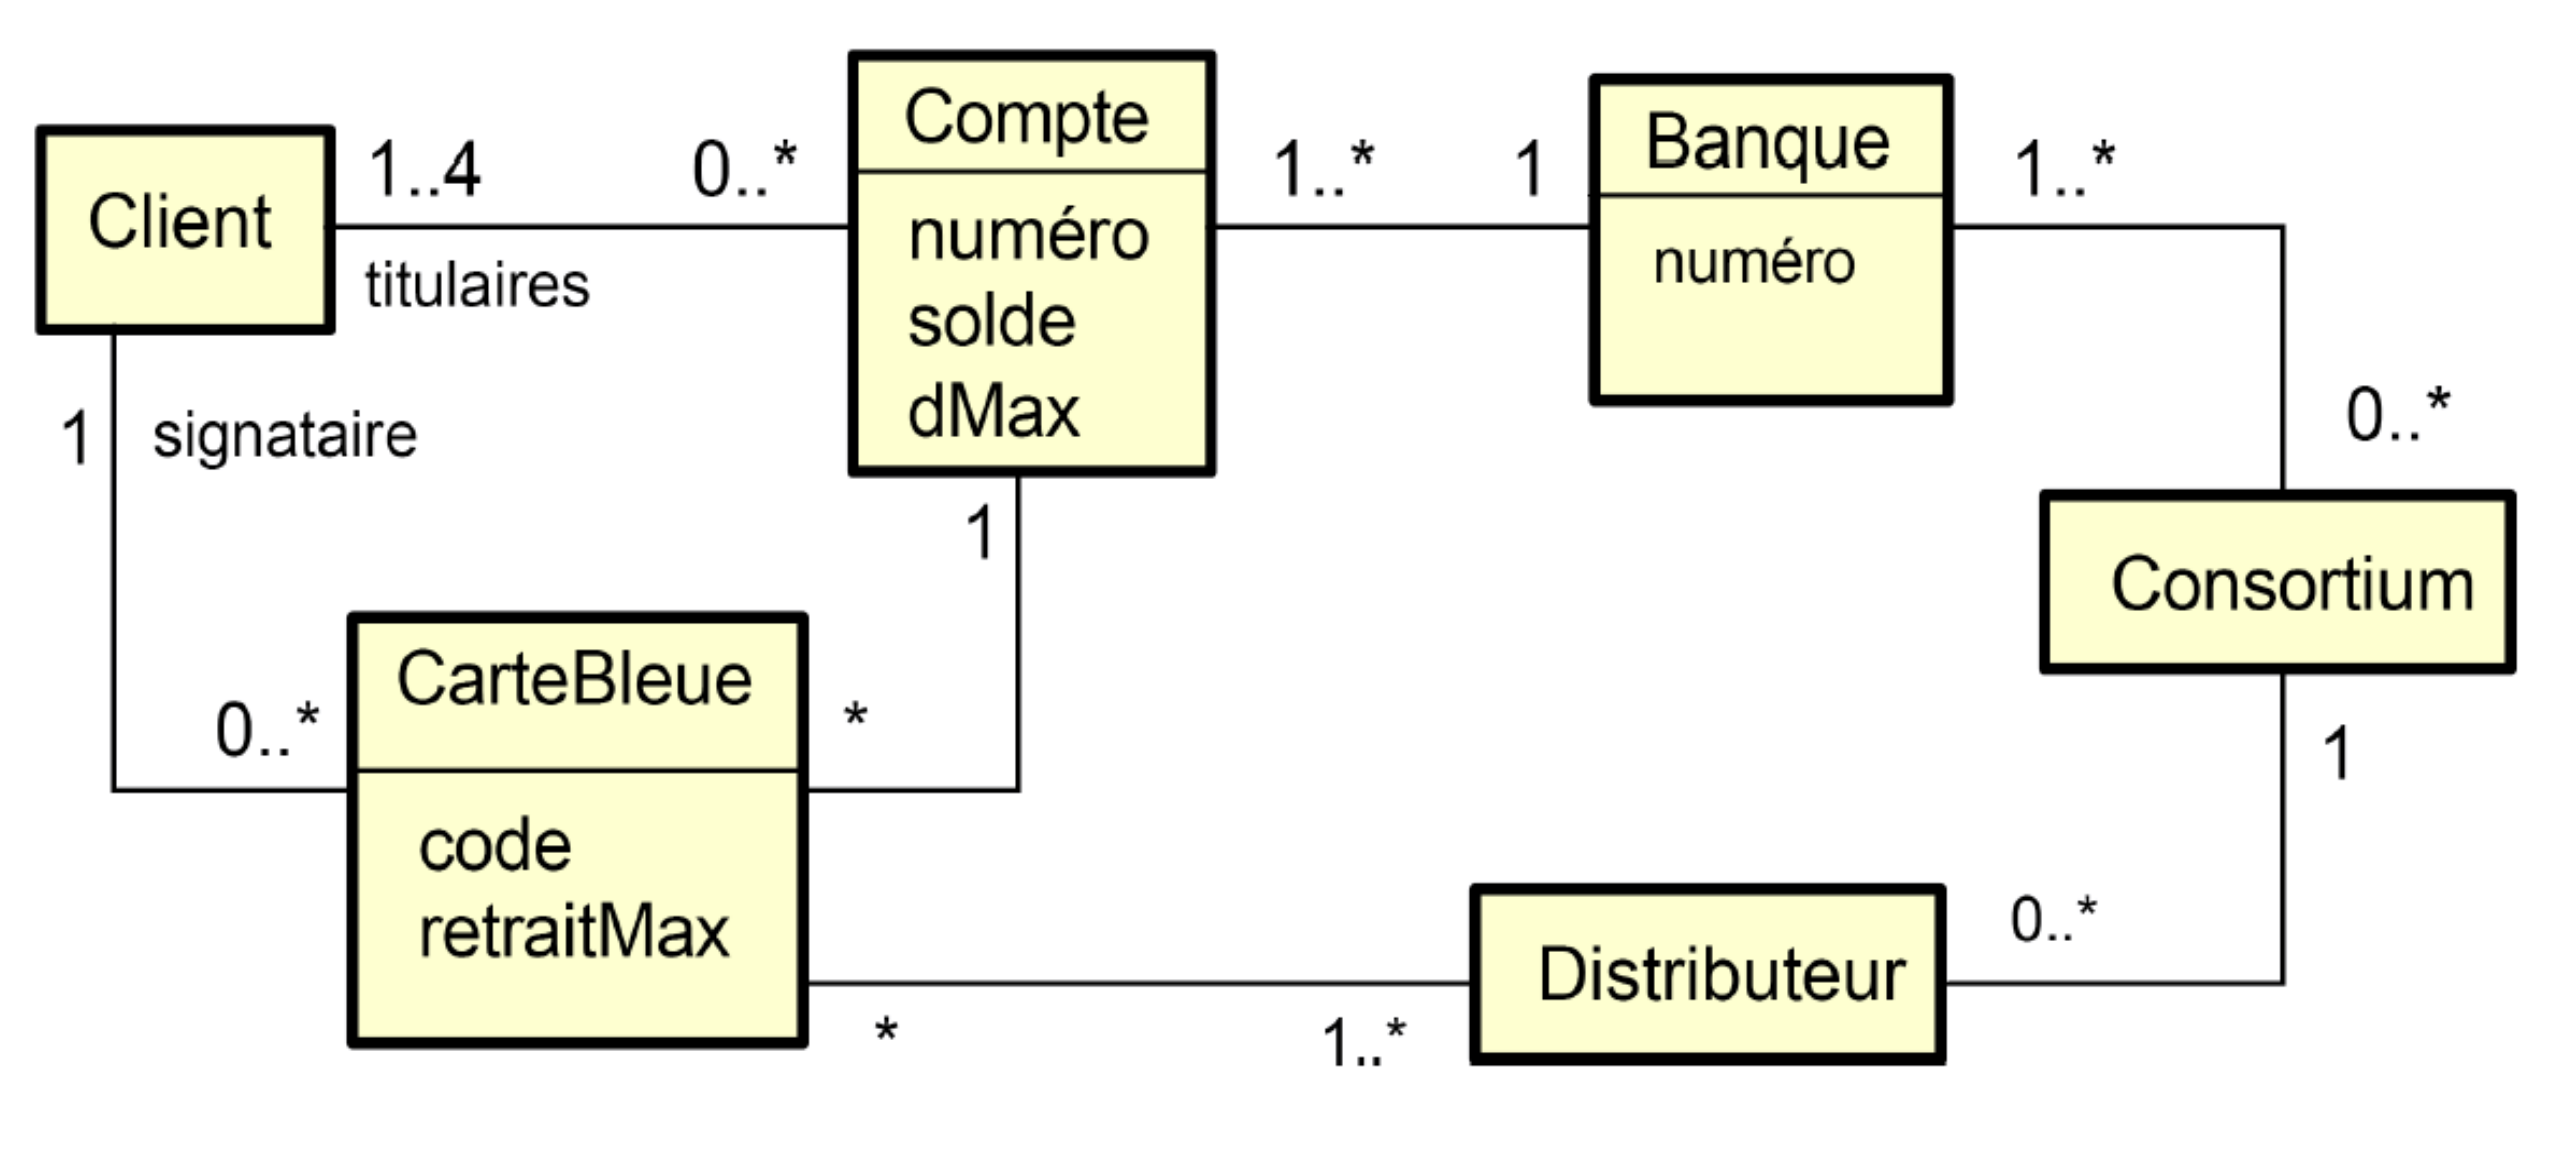
\includegraphics[width=0.45\textwidth]{ClassDExo1.png}
            \end{center}
        \end{figure}

\begin{lstlisting}
context Compte 
inv : solde >= dMax 

context CarteBleue 
inv : signataire = compte.titulaires 

context CarteBleue 
inv : compte.titulaires -> includes(signataire)
--Si l'objet titulaires est une collection de plusieurs 
--titulaires possible

context CarteBleu
def estAccepte(a : CarteBleue) : 
Boolean = (distributeur = compte.banque.consertium.distributeur) 

inv: estAccepte(self) 
\end{lstlisting}



            \begin{Exercice}{}{}
                Soit les contraintes suivantes, 
                \begin{enumerate}
                    \item Toutes les équipes doivent avoir au moins un enfant
                    \item Toutes les équipes doivent avoir gagné au moins un match
                    \item Toutes les équipes professionnelles doivent avoir participé à au moins 
                    un tournoi professionnel
                \end{enumerate}
                Écrire les contraintes OCL
            \end{Exercice}
        

            \begin{figure}[H]
                \begin{center}
                    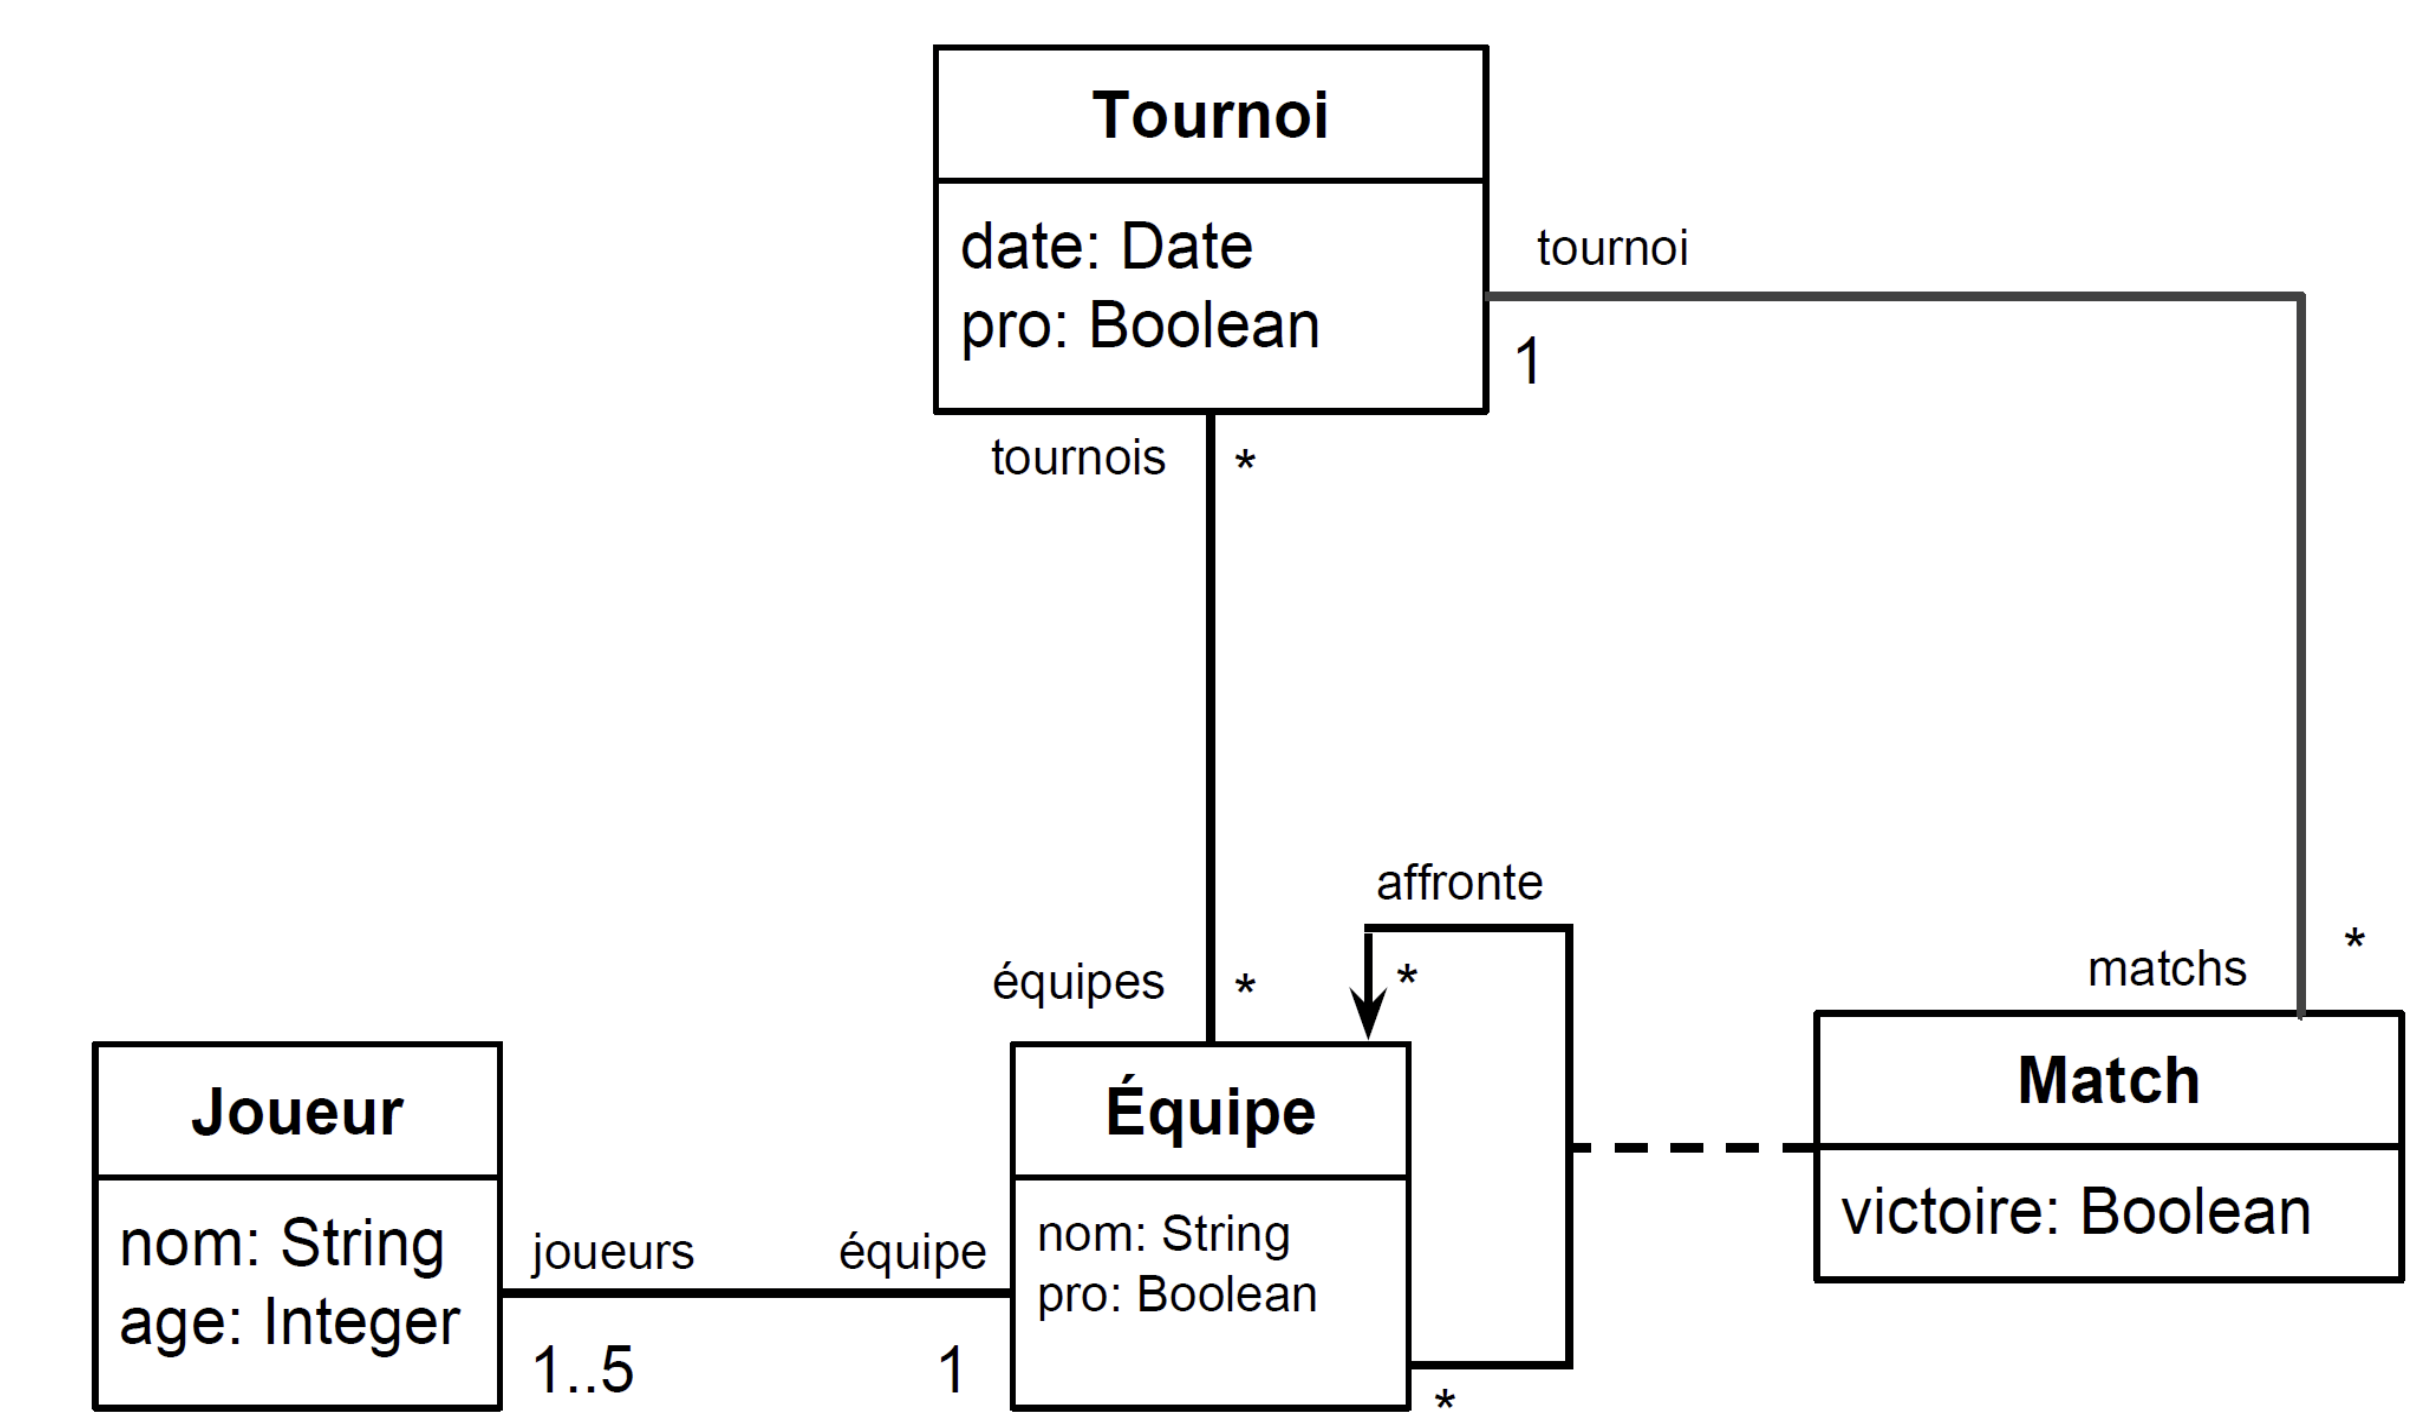
\includegraphics[width=0.45\textwidth]{ClassDExo2.png}
                \end{center}
            \end{figure}

\begin{lstlisting}
context Tournoi 
inv : self.equipes -> 
forall(e | e.joueurs -> exists(j | j.age < 18 ))

--Toutes les equipes du Tounoi on un joueur tel 
--son age est inferireur a 18 ans (est un enfant)

context Tournoi 
inv : self.equipes -> 
forall(e | e.matches -> exists(m | m.victoire = true))
--Toutes les equipes du Tournoi ont des matchs tel 
--qu'au moin un de ces matchs est une victoire.

context Tournois 
inv: self.equipes ->
forall(e | e.pro implies e.tournois->exists(t | t.pro))
--Toutes les equipes professionnelles ont participes 
--a un tournoi professionnelles


context Equipe
def: participatedInProTournament : Boolean = 
    self.tournois->exists(t | t.pro)

context Equipe
inv: 
    self.pro implies self.participatedInProTournament
-- Facon alternative en utilisant une def.


context Tournoi 
inv : self.equipes -> 
forall(e | (e.pro = True) implies e.joueurs -> 
(forall(j | j.age > 18)))
--Toutes les equipes professionnelles sont 
--composees de joueurs majeurs



context Equipe 
def: allPlayersAdults : Boolean = 
    self.joueurs -> forall(j | j.age >= 18)

inv : self.equipes -> 
forall(e | e.pro implies e.allPlayersAdults)
-- Facon alternative en utilisant une def. 

context Equipe
inv: self.joueurs->isUnique(j | j.nom)
--Deux joueurs dans la meme equipe ne peuvent pas 
--avoir meme nom.


context Tournoi
inv: self.equipes.joueurs->flatten()->
isUnique(j | j.nom)
--S'assure que deux joueurs qui participent au meme 
--tournoi n'ont pas le meme nom. 
-- flatten() recupere tous les nom de tous les joueur et en 
-- fait une seule collection

\end{lstlisting}

\begin{lstlisting}
--Le service (Somme des heures effectuees) fait 
--par un enseignant.
context Enseignant:: service : 
    Integer derive : self . enseigne . heures->sum()


--Quelque soit la matiere, il y a toujours au moins un 
--enseignant qui la maitrise.
context Matiere inv: self .est_maitrisee ->notEmpty()

--La methode augmenterSal(m :Integer) qui augmente
--le salaire d'un enseignant, d'un montant m.
context Enseignant::augmenterSal(m : Integer) 
post: self . salaire = self . salaire @pre + m


--Il y a un et un seul chef par departement et son age 
--depasse les 40 ans.
context Departement inv: 
    self . chef->size() = 1 and self . chef .age > 40


--Le nom de chaque enseignant est unique
context Departement inv: 
    self . enseignants->
    forAll(e1, e2 : Enseignant|e1 <>e2 implies
e1.nom <>e2.nom)


-- Dans chaque departement, il existe au moins 
-- un professeur
context: Departement inv: 
    self . enseignants->
    exists(e: Enseignant |e.titre = Titre ::Pr)


--Un professeur a toujours 100% de reussite
context Enseignant let : 
    etuds () : Bag(Etudiants) = 
    self . enseigne . etudiant
    inv: self . titre = Titre :: 
    pr implies self . etuds ()->
    forAll(e| e.estAdmis())
--Un etudiant est admis si la moyenne de toutes 
--ses notes est superieure ou egale a 10.
context Etudiant inv : self.note[matiere]->moy()>=10
    
\end{lstlisting}


\chapter{Architecture \texttt{\S\;  Amal 15}}

        \section{Conceptions Architecturale}

        \begin{Concept}{La conception architecturale}{}
            Il s'agit d'une prendre des décisions qui nous permettent d'avoir un \textbf{aperçu de haut niveau}
            du système. On définit les \textcolor{myb}{composants} principaux, leurs propriétés et leurs collaborations. 
            Ont fait la conception des \textcolor{myb}{interfaces utilisateurs}, des \textcolor{myb}{bases de données},
            des \textcolor{myb}{points de contrôle} (permettent les correction, la sécurité, la tolérance des fautes, 
            la protection des données, etc.). On fait la conception des \textcolor{myb}{réseaux} qui 
            régissent la communication entre des processus. On planifie aussi l'allocation de chaque composant 
            aux \textcolor{myb}{ressources matérielles}.  
        \end{Concept}


        \section{Propriétés d'une conception de bonne qualité}
        \begin{itemize}
            \item \textbf{Réutilisation}  
                \begin{itemize}
                    \item[$\blacktriangleright$] Il est possible de réutiliser un composant d'un produit 
                        pour faciliter le développement d'un autre produit ayant des fonctionnalité différentes.
                \end{itemize}
            \item \textbf{Conception modulaire}  
                \begin{itemize}
                    \item[$\blacktriangleright$] 
                        Le logiciel est décomposé en modules \textbf{indépendant et interchangeables} qui contiennent
                        tout ce qui est nécessaire pour exécuter un aspect d'une fonctionnalité. 
                    \item[$\rhd$] Les modules sont cohésif et faiblement couplé
                    \item[$\rhd$] Les modules sont réutilisables
                \end{itemize}
            \item \textbf{Maintenabilité}   
                \begin{itemize}
                    \item[$\blacktriangleright$] Le logiciel est tel qu'il n'y a pas beaucoup de modifications à 
                        apporter après le développement initial. 
                \end{itemize}
       \end{itemize}       

       \section{Propriétés d'une mauvaise conception}
                
            \begin{itemize}
            \item \textbf{Rigidité}  
                \begin{itemize}
                    \item[$\blacktriangleright$] Locigiel difficile à modifier parce chaque changement 
                        \textbf{impacte beaucoup trop} d'autres parties du système  
                \end{itemize}
            \item \textbf{Fragilité}  
                \begin{itemize}
                    \item[$\blacktriangleright$] Quand on effectue une modification, des parties du système ne 
                        fonctionnent plus de façon imprévisible
                \end{itemize}       

            \item \textbf{Immobilité}  
                \begin{itemize}
                    \item Il est difficile de réutiliser un composant dans une autre application.  
                \end{itemize}
            \end{itemize}

        \section{Réutiliosation de logiciel}
        On distingue la réutilisation \textbf{opportuniste} de celle qui est \textbf{systématique}. La première 
        survient lorsque qu'on finit par réutiliser accidentellement des parties du système lors 
        du développement. La second survient lorsqu'on planifie et conçoit des composants délibéremment 
        réutilisables. 
        
        \paragraph{}
        Il faut considérer la réutilisation en se demandant s'il existe des composants développés à 
        l'interne qui pourraient être utiles; s'il y a des composants ou librairies en vente libre disponibles
        qui peuvent aider à implémenter les exigences ou si les interfaces pour les composants 
        sont compatibles avec l'architecture du système. 

        \begin{note}{}{}
            Il est estimé que seul 15\% du nouveau code contribue à un objectif origianal ; 
            85\% peut être standardisé et réutilisé. Notons aussi que la réutilisation affecte 
            la maintennace et le développement. 
        \end{note}

        Le \textbf{but premier} de la maintenance est de \textbf{faciliter la maintenance}. Il faut considérer 
        les questions suivantes :
        \begin{itemize}
            \item Est-ce important que ce soit l'équipe qui implémente un composant ou peut-on réutiliser 
                un composant existant et ainsi faciliter le développement ? (biais de \textit{ce n'est pas moi qui 
                l'ai fait})
            \item Est-ce que les \textbf{craintes} sont fondées ou est-ce que les composants existants sur 
                le marché sont fiables ?
            \item Que coutera l'utilisation de composant existant en termes de : 
                \begin{itemize}
                    \item[$\blacktriangleright$] Temps nécessaire pour comprendre le composant 
                    \item[$\blacktriangleright$] Coût du composant 
                    \item[$\blacktriangleright$] Temps de planification 
                    \item[$\blacktriangleright$] Problèmes légaux 
                    \item[$\blacktriangleright$] Manque de couverture de code source
                \end{itemize}
        \end{itemize}

        \section{Exemples et framework}

        \begin{Definitionx}{}{}
            Les \textbf{framework} sont des plateformes qui incorporent une \textit{logique de contrôle générique}. 
            Les utilisateurs font appels à des fonctionnalité qui y sont disponibles. Il peut aussi 
            personaliser son framework en utilisant des programmes spécifiques à ses besoins d'usage : des
            \textit{plugin}.
        \end{Definitionx}

        \begin{EExample}{Framework populaires}{}
            Leaflet, JQuery, Lo, DjangoDB, .NetCore, Laravel, etc. 
        \end{EExample}

        \begin{Definitionx}{Programmation orienté composant}{}
           Méthodologie qui consiste à concevoir en \textbf{assemblant des composants} fortement encapsulés 
           avec un interface concise et rigoureuse. 
           \begin{itemize}
            \item \textbf{La décomposition horizontale}  
            \item \textbf{La décomposition verticale}  
           \end{itemize}
           La première approce divise le problème en un ensembles d'objets représentés par des types 
           de données abstrait. La second approche engendre des niveaux d'abstractions de plus en plus 
           élémentaires. L'objectif ultime est de \textbf{favoriser la réutilisation}.  
        \end{Definitionx}

        \section{Integration de composant}
        Pour intégrer un composant au système, il faut se questionné quant à la capacité 
        du système à faire interface avec l'architecture du et l'environnement externe ; se demander 
        si les échanges de données sont compatibles entre composants ; déterminer les 
        \textcolor{myb}{activités communes} aux composants ; déterminer la méthode de gestion et d'accès 
        aux \textcolor{myb}{ressources} ; prévoir de \textcolor{myb}{nouvelle intégrations} ; concevoir 
        le système de façon à ce qu'il est possible d'ajouter de \textcolor{myb}{nouveaux composants}.

        \section{Styles d'architecture}
        \begin{itemize}
            \item Pipe et filtre 
            \item Par couche 
            \item Client-serveur 
            \item Modèle-Vue-Contrôleur 
            \item Peer-to-peer 
            \item Cloud
        \end{itemize}


\paragraph{Pipe et Filtre}
Ce style architectural consiste en une série de composants de traitement (filtres), reliés par des chemins de données (pipes). Chaque filtre traite ses données d'entrée et les passe au filtre suivant. Il est couramment utilisé pour les traitements en flux, s'inspirant des pipelines de shell Unix.

\paragraph{Par Couches}
Dans cette architecture, le logiciel est organisé en couches hiérarchiques. Chaque couche fournit des services à celle du dessus et utilise ceux de la couche inférieure, favorisant ainsi organisation et séparation des préoccupations.

\paragraph{Client-Serveur}
C'est une structure d'application distribuée séparant les tâches entre les fournisseurs de services (serveurs) et les demandeurs (clients). Les clients envoient des requêtes aux serveurs qui traitent et retournent les informations. Ce modèle est fondamental pour de nombreuses applications web.

\paragraph{Modèle-Vue-Contrôleur (MVC)}
Le MVC sépare une application en trois composants : le Modèle (données), la Vue (interface utilisateur) et le Contrôleur (logique métier). Cette séparation aide à gérer des applications complexes, facilitant la réutilisation de code et le développement parallèle.

\paragraph{Pair à Pair (P2P)}
Dans un réseau P2P, chaque participant agit à la fois comme un client et un serveur, permettant une interaction directe et le partage de ressources sans serveur central. Ce style est populaire dans les réseaux de partage de fichiers et la technologie blockchain.

\paragraph{Cloud}
L'architecture cloud se réfère aux composants nécessaires pour le cloud computing, comprenant l'interface utilisateur, le backend, le réseau et la livraison basée sur le cloud. Elle offre des services informatiques à distance évolutifs et


        \section{Compromis du client}
        Lors des workflow, plusieurs stratégies peuvent être employées pour s'assurer que l'architecture 
        est valide tout en respectant les exigences du client. 
        On offre au client le choix de : revoir certaines exigence, augmenter le budget, repousser la date 
        de livraison. 

            \section{Importance de l'architecture}

            \begin{itemize}
                \item Le workflow des exigences peut être corrigé durant 
                    le workflow d’analyse 
                \item Le workflow d’analyse peut être corrigé durant le workflow de 
                    conception
                \item Le workflow de conception peut être corrigé durant le 
                    workflow d’implémentation
            \end{itemize}

            Mais \textbf{il n’y a pas moyen de surmonter une architecture non-optimale plus tard}. 
            Il faut absolument reconcevoir l’architecture immédiatement !


            \chapter{Paradigme Orienté Objet \texttt{\S \; Amal 16}}  


            \section{Classe}
            \begin{Definitionx}{Classe}{}
                Une \textbf{classe} est une \textbf{représentation d'un ensemble d'objets} qui 
                partaent une \textcolor{myb}{structure} un \textcolor{myb}{comportement} et 
                une \textcolor{myb}{sémantique} similaires. Tous les objets instanciés à partir d'une même classe 
                sont \textbf{structurelement similaires}.  
            \end{Definitionx}


            \begin{note}{}{}
                Les objets appartenant à une classe sont des \textbf{instances} de cette classe.   
            \end{note}
            
            \section{Objet}
            \begin{Definitionx}{Objet}{}
                Un \textbf{objet} représente une \textbf{entité} \textcolor{myb}{réelle} ou 
                \textcolor{myb}{conceptuelle} \textbf{singulière} et \textbf{identifiable} ayant 
                un \textbf{rôle} ou plusieurs rôles bien définis.   
            \end{Definitionx}

            \begin{note}{}{}
                Les connections \textbf{physiques} ou \textbf{conceptuelles} entre les objets permettent 
                la communication et les interactions entre ceux-ci; ils \textbf{collaborent} ainsi
                pour accomplir la tâche voulue. 
            \end{note}

            \begin{definition}{Message}{}
                Véhicule par lequel un objet expéditeur \textbf{transmet une information} 
                à un objet cible. 
            \end{definition}                    


            \section{Distinction entre classe et objet}

            Les \textbf{classes} sont \textcolor{myb}{statiques} et évaluées lors de la compilation. 
            Il existe \textcolor{myb}{une seule copie} d'une classe en mémoire et la mémoire 
            pour \textbf{stocker les méthodes} est allouée \textcolor{myb}{une seule fois}.     
            
            Les \textbf{objets} sont \textcolor{myb}{dynamiques} et créés lors de l'exécution. Une 
            copie de l'objet est créée à \textcolor{myb}{chaque fois} que la classe est instanciée.   
            a mémoire pour \textbf{stocker les attributs} est allouée \textcolor{myb}{pour chaque
            objet instancié}.     


            \section{Héritage}
            \begin{Definitionx}{Héritage}{}
                Relation de \textcolor{myb}{partage de structure et de comportement}. Les objets héritant tous 
                d'une classe commune possède toutes les méthodes et attribut de cette classe. 
            \end{Definitionx}

            \begin{note}{}{}
                L'héritage a multiples \textbf{utilitées}, notamment la réutilisation de fonctionnalité ; 
                permet d'implémenter des fonctionalité dinstinctes entre les objets ayant le même 
                parent en partant d'un cannevas, plutôt qu'en partant de rien. 
            \end{note}


            \section{Modificateur d'accès}
            \begin{Definitionx}{Modificateur d'accès}{}
                Ils définissent la \textbf{visibilité} des attributs et méthodes pours les autres objets
            \end{Definitionx}

            \begin{itemize}
                \item \textbf{Private}    
                    \begin{itemize}
                        \item[$\blacktriangleright$] Accès permis seulement aux objet de la classe
                    \end{itemize} 
                \item \textbf{Protected}  
                    \begin{itemize}
                        \item[$\blacktriangleright$] Accès permis uniquement aux objet de la classes et aux objets 
                            enfants. 
                    \end{itemize}
                \item \textbf{Public}  
                    \begin{itemize}
                        \item[$\blacktriangleright$] Accès permis à tout le monde. 
                    \end{itemize}
                \item \textbf{Package}  
                    \begin{itemize}
                        \item[$\blacktriangleright$] Accès \textcolor{myb}{par défaut} lorsque qu'aucune déclaration 
                            d'accès n'est faites. 
                    \end{itemize}
            \end{itemize}

            \begin{note}{}{}
                Les enfants n'ont pas accès à toutes les propriétés du parents. Les propriétés privées 
                ne sont pas accessibles pour les enfants. 
            \end{note}

            \section{Overriding}

            \begin{Definitionx}{Overriding}{}
                \textbf{Redéfinition} d'une méthode d'un parents. Syntaxe : \texttt{@Override}    
            \end{Definitionx}


            \section{Polymorphisme}
            Un exemple de polymorphisme est lorsqu'une méthode prend différente forme dans différentes classes. 
            Deux classes \texttt{Triangle} et \texttt{Rectangle} pourraient hériter du même parent 
            \texttt{Polygone} et de la même méthode parent \texttt{computeArea}. Si chacune de ses classes 
            redéfinit la méthode \texttt{computeArea} pour l'adapter aux objet \texttt{Triangle} et 
            \texttt{Rectangle}, il s'agit d'une forme de polymorphisme.   

            \section{Abstraction}
            Une classe ou une méthode abstraite généralise un ensemble de classes en définissant les 
            \textcolor{myb}{éléments communs} pour ainsi laisser les enfants définir les éléments spécifiques. 
            \begin{Syntaxe}{Abstraction}{}
                \texttt{abstract}  
            \end{Syntaxe}


\begin{EExample}{Ok}{}
    
\begin{lstlisting}[style=JavaDraculaWhite]
    public abstract class Forme {
        private String couleur; 

        public Forme() {...} 
        public String getColor() { 
            return couleur; //Implementation par defaut
        }
        //Methode abstraite : pas de code 
        //Seulement une signature et un type retourn
        public abstact double aire();

    } 

    public class Cercle extends Forme {
        @Override 
        public double aire() {
            returnb Math.PI * rayon * rayon; 
        }
    }
    
    public class Rectangle extends Forme { 
        @Override 
        public double aire() {
            return largeur * hauteur
        }
    }

    public class Triangle extends Forme { 
        @Override
        public double aire() {
            return largeur * hauteur / 2.0;
        }
    }

\end{lstlisting}
\end{EExample}


        \section{Encapsulation}

        \begin{Definitionx}{Encapsulation}{}
            La notion d'encapsulation est le principe par lequel on regroupe des concepts similaires. 
            On crée des \textbf{abstraction} qui \textcolor{myb}{encapsulent} l'essence d'éléments 
            partagent un sens commun. La \textbf{création de classe} et la \textbf{définition de types} 
            de données sont des exemples d'encapsulation. 
        \end{Definitionx}               

        \section{Raffinement par étrape}

        \begin{Concept}{Rafinnement par étape}{}
            Principe par lequel on effectue la conception en priorisant les concepts de 
            \textbf{haut niveau}. On suppose l'existance de niveau plus bas et visualise 
            comment ceux-ci peuvent être encapsulés par des niveaux supérieurs. 
            Dans une deuxième phase, on s'intéresse ensuite aux détails de l'implémentation 
            des plus bas niveau ; on prend des décision spécifiques qui permettent de concrétiser 
            ces niveaux plus bas. Le principe de \textbf{rafinnement par étape} est donc \textcolor{myb}{récursif}.      
        \end{Concept}

        \section{Dissimulation}


        \begin{figure}[H]
            \begin{center}
                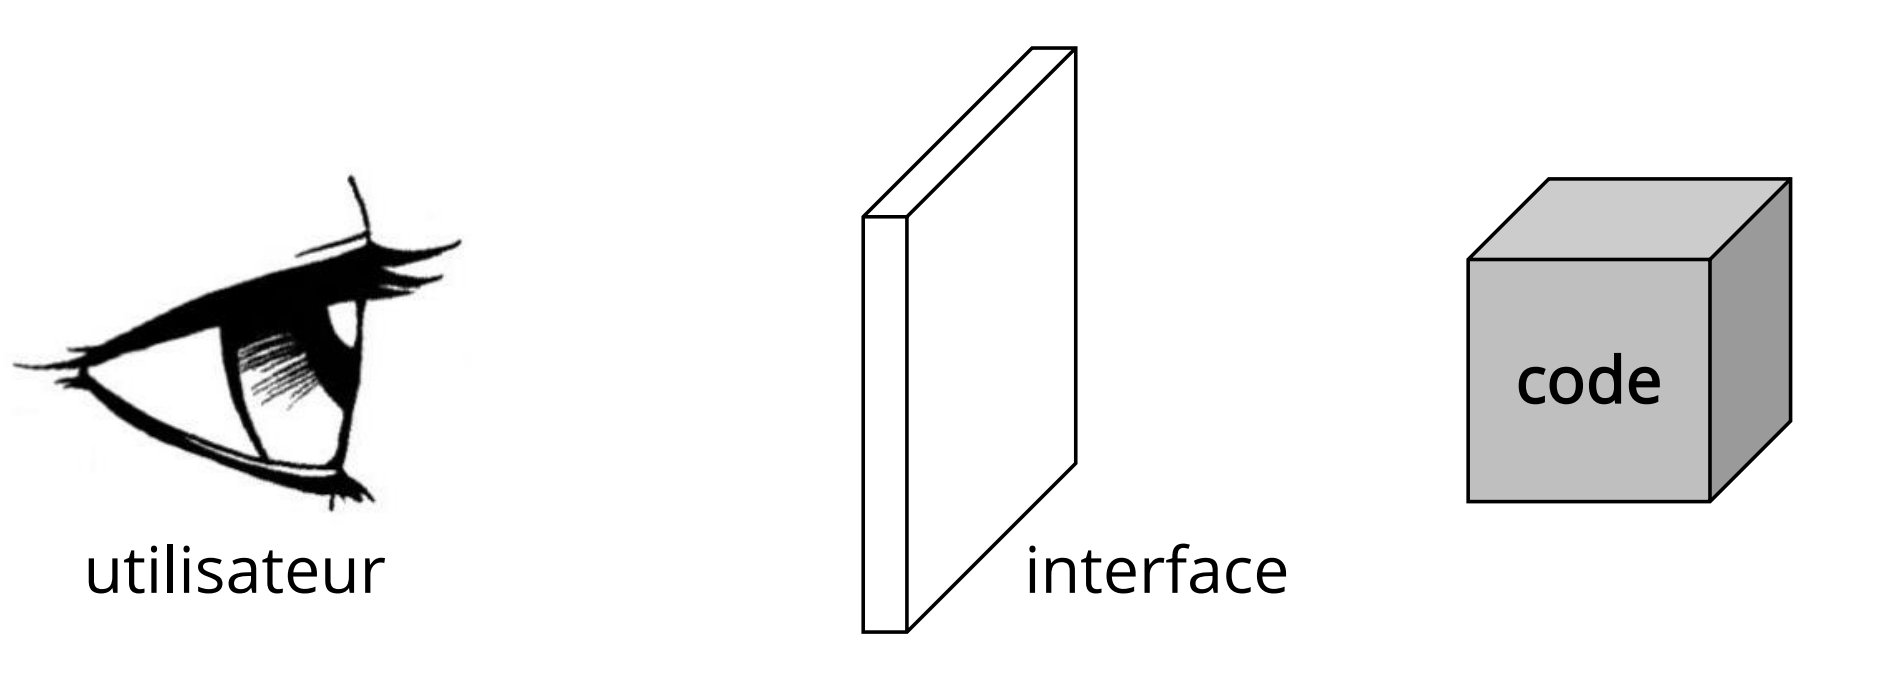
\includegraphics[width=0.45\textwidth]{SpaguettiCode.png}
            \end{center}
        \end{figure}
        On restreint la vue de l'utilisateur sur l'informatio ou l'implémentation. 
        Pour accéder à une information, l'utilisateur utilise les méthode publiques. 
        Par ailleurs, l'utilisateur peut utiliser une méthode sans savoir comment elle trait le contenu. 

        \begin{note}{}{}
            Utiliser des getters et setters est une \textbf{bonne pratique}  
        \end{note}
        

        \section{Avantages de l'OOP}

        \begin{itemize}
            \item \textbf{Concepteur et utilisateur sont indépendants}
                \begin{itemize}
                    \item[$\blacktriangleright$] Ils doivent uniquement s’entendre sur \textcolor{myb}{l’interface}
                \end{itemize}
            \item \textbf{L’évolution du logiciel est plus facile}
                \begin{itemize}
                    \item[$\blacktriangleright$] Changements futurs anticipés/contrôlés
                \end{itemize}
            \item \textbf{Abstraction de l’utilisateur est élevée}
                \begin{itemize}
                    \item[$\blacktriangleright$] Il n’a plus à s’occuper de comment ça fonctionne
                \end{itemize}
            \item \textbf{La réutilisation du code est plus facile}
                \begin{itemize}
                    \item[$\blacktriangleright$] Design modulaire
                \end{itemize}
            \item \textbf{Favorise la dissimulation des détails et oblige à dépendre d’interfaces publiques}
                \begin{itemize}
                    \item[$\blacktriangleright$] Modificateurs privés, classes abstraites, interfaces                
                \end{itemize}
        \end{itemize}


        \section{Désavantages de l'OOP}

        \begin{itemize}
            \item Prolifération de fichiers (un par classe, généralement )
            \item Pas idéal pour le développement d’interfaces graphiques
            \item Classe à la base de la hiérarchie est fragile aux modifications
        \end{itemize}


        \chapter{Patrons de conception \texttt{\S \; Amal 17}  }


        \begin{Definitionx}{Patron de conception}{}
            Une \textbf{patron de conception} décrit une \textcolor{myb}{solution générale à un problème}  
            La solution proposée est modifiée ou adaptée selon les legociels et les langages de programmation 
            choisis, au besoin
        \end{Definitionx}

        \begin{note}{}{}
            \textbf{L'objectif} est d'accroître la qualité du code en visant la \textcolor{myb}{flexibilité}, 
            la meilleure \textcolor{myb}{compréhension et performance}, \textcolor{myb}{la fiabilité accrue}.    
        \end{note}


        \begin{figure}[H]
            \begin{center}
                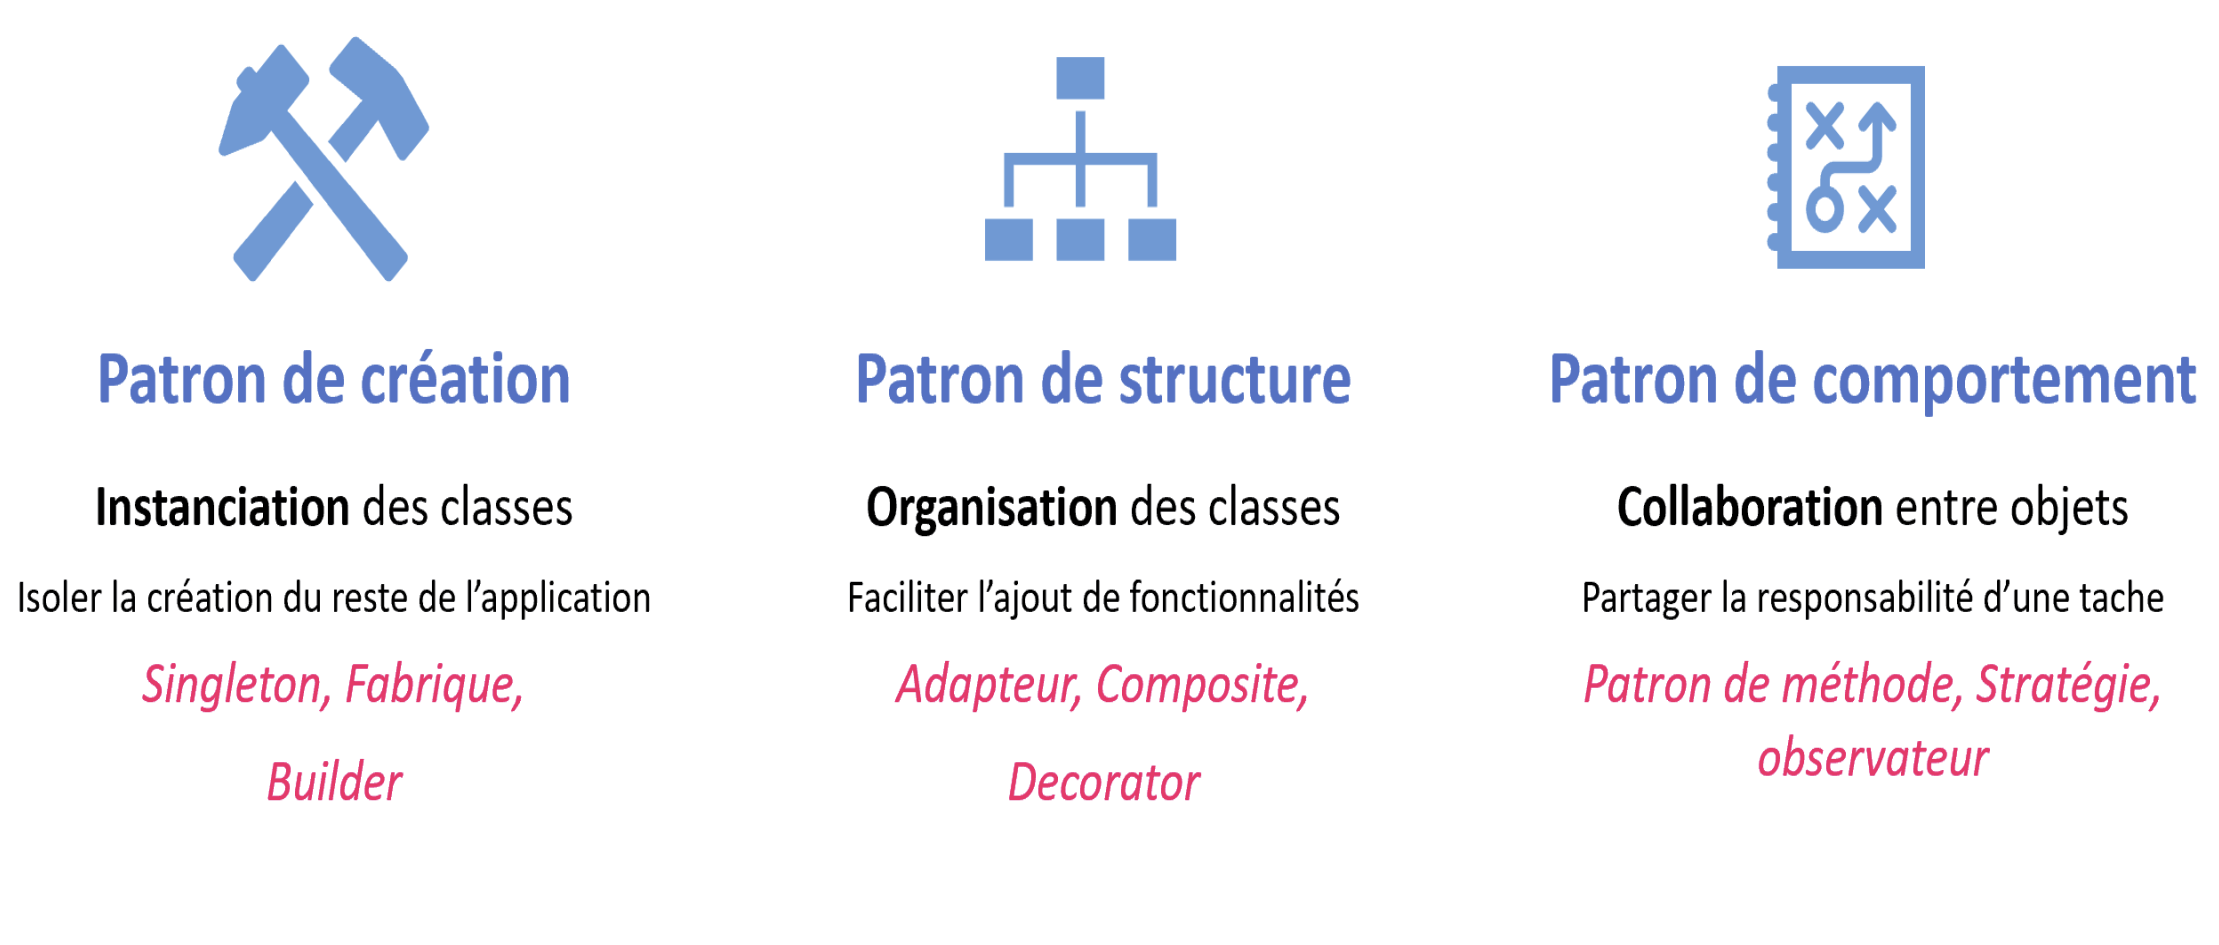
\includegraphics[width=0.45\textwidth]{patronTypes.png}
            \end{center}
        \end{figure}


        \section{Patron Singleton}

        \begin{Definitionx}{Patron Singleton}{}
            \textbf{Singleton} est un modèle de conception de création qui vous permet de vous
            assurer qu'une classe a une seule instance, tout en fournissant un \textcolor{myb}{point d'accès
            global} à cette instance.

        \end{Definitionx}   


        \begin{Definitionx}{Accès global}{}
            Comme une variable globale, le modèle Singleton vous permet
            d'accéder à un objet depuis n'importe où dans le programme. Cependant, il
            protège également cette instance contre l'écrasement par un autre code.
        \end{Definitionx}


        \begin{EExample}{Un Singleton}{}
            La classe Singleton déclare la méthode statique \texttt{\textcolor{myb}{getInstance}} 
            qui retourne la même \textbf{instance de sa propre classe}. 
            Il faut : 
            \begin{itemize}
                \item Rendre le constructeur par défaut privé, pour empêcher d'autres objets 
                    en utilisant le nouvel opérateur avec la classe Singleton.
                \item Créez une méthode statique qui agit comme un constructeur.
            \end{itemize}

\begin{lstlisting}[style=JavaDraculaWhite]
public class Singleton {
    private static Singleton _instance; 
    private Singleton() {}

    public static Singleton getInstance() {
        if (_instance ==  null) {
            _instance = new Singleton();
        }
        return _instance;
    }

}
\end{lstlisting}
        \end{EExample}                  

        \begin{note}{}{}
            On peut utiliser le patron \textbf{Singleton} pour \textit{implémenter un} \texttt{IdManager} unique qui 
            crée des ID grâce à l'implémentation de \texttt{generateID()}. Puisque l'ID Manage est 
            un singleton, seul lui est reponsable de la génération d'ID et chaque ID sera unique, 
            puisque la valeur est incrémentée chaque fois qu'un ID est distribué.
        \end{note}

        \begin{EExample}{implémentation de \texttt{IdManage} selon le patron Singleton  }{}


\begin{lstlisting}[style=JavaDraculaWhite]
private classe IdManager {
    private static IdManager _instance = new IdManager(); 
    private string lastID; 
    private IdManager() {
        this.lastID = -1;
    }

    public static IdManager getInstance() {
        return _instance
    }

    public String generateID() {
        return ++this.lastID;
    }

}
\end{lstlisting}
        \end{EExample}      
        \section{Patron adapteur}


        \begin{Concept}{Interface Wrapper}{}
            Un Wrapper est une interface qui permet la communication entre deux classes 
            dont \textcolor{myb}{l'envoie d'un message} de la première est incompatible avec la 
            \textcolor{myb}{réception} du message de la seconde. P. ex., le nombre d'arguments 
            offerts par une méthode est incompatible avec le nombre d'argument que cette méthode prend 
            normalement.
        \end{Concept}


\begin{lstlisting}[style=JavaDraculaWhite]
public class Insurance {
        public void determinerPremier() {
            /Offre 2 arguments mais Objet appliquant 
            de type NeutralApplicant a une methode qui 
            prend uniquement 1 argument */ 

            appliant.computePremium(age, gender)
        }
}
public class NeutralApplicant {
        public void computeNeutralPremium(age)
}
\end{lstlisting}

\textbf{Solutionné par un \texttt{Wrapper}} :     



\begin{lstlisting}[style=JavaDraculaWhite]
public class Wapper {
    computePremium(age, gender) {
        neutralApplicant.computeNeutralPremium(age);
    }
}
public class Insurance {
        public void determinerPremier() {
            /Offre 2 arguments et appel Wrapper qui  
            a son tour appel la methode de NeutralApplicant */ 

            Wrapper.computePremium(age, gender)
        }
}
public class NeutralApplicant {
        public void computeNeutralPremium(age)
}
\end{lstlisting}

        \begin{note}{}{}
            L'adaptateur ou \texttt{Wrapper}  fournit tous les avantages de la \textcolor{myb}{dissimulation de
            l’information} sans avoir à cacher ses détails d’implémentation
        \end{note}          


        \begin{EExample}{Implémentation d'adapteur}{}
            \textbf{Problème} :
            \vspace{1em}\\
            \texttt{naSocket.\textcolor{red}{outputToPlug}(euPlug)} engendrera une erreur ; 
            La méthode \texttt{outputToPlug} doit prendre en argument un objet de type 
            \textcolor{myb}{NorthAmericanPlug} mais reçoit un objet de type \textcolor{myb}{EuropeanPlug}

\begin{lstlisting}[style=JavaDraculaWhite] 
public class NorthAmericanPlug {
    public String getNAVoltage() {
        return "110V";
    }
}
public class EuropeanPlug {
    public String getEUVoltage() { 
        return "220V";
    }
}
public class Socket {
    public String outputToPlug(NorthAmericanPlug plug) {
        return "Delivering power to " + plug.getNaVoltage();
    }
}
public class Client {
    public static void main(String[] args) {
        Socket naSocket = new Socket(); 

        NorthAmericanPlug naPlug = new NorthAmericanPlug(); 
        System.out.println(naSocket.outputToPlug(naPlug));

        EuropeanPlug euPlug = new EuropeanPlug(); 
        // Ligne fautive (erreur)
        System.out.println(naSocket.outputToPlug(euPlug))
    }
}

/*Solution : Creer un PlugAdapter qui extends 
NorthAmericanPlug et Override getNaVoltage ; 
la nouvelle methode appelle getEUVoltage 
sur un objet EuropeanPlug propre a PlugAdapter */  

public class PluygAdapter extends NorthAmericanPlug {
    EuropeanPlug euPlug; 

    public PlugAdapter() {
       euPlug = new EuropeanPlug(); 
    }

    @Override
    public String getNaVoltage() {
        return euPlug.getEUVoltage();
    }
}
public class Client {
    public static void main(String[] args) {
        Socket naSocket = new Socket(); 

        NorthAmericanPlug naPlug = new NorthAmericanPlug(); 
        System.out.println(naSocket.outputToPlug(naPlug));

        PlugAdapter euPlugAdapter = new plugAdapter(); 
        // Correction
        System.out.println(naSocket.outputToPlug(euPlugAdapter))
    }
}


\end{lstlisting}

        \end{EExample}              

    \section{Patron Composite}
    Une méthode composite itère généralement sur une collection de composants en 
    invoquant la méthode approprié sur chaque composant. Dans l'exemple suivant,  
    la methode \texttt{parenthesize()} d'un objet de type \texttt{Manager} itère 
    sur le \textcolor{myb}{composant} de \texttt{Manager} et appelle la méthode 
    \texttt{parenthesize()} des composants qui peut être une méthode d'un autre 
    \texttt{Manager} ou d'un \texttt{Employee}.     


    \begin{EExample}{Patron composite dans la hiérarchie d'une compagnie}{}
        
\begin{lstlisting}[style=JavaDraculaWhite]
 public abstract class Employee {
    protected String name;
    protected double salary;

    public String getName() {
        return name;
    }

    public void setName(String name) {
        this.name = name;
    }

    public double getSalary() {
        return salary;
    }

    public void setSalary(double salary) {
        this.salary = salary;
    }

    public abstract String parenthesize();
}

public class Developer extends Employee {
    public Developer(String name) {
        this.name = name;
    }

    @Override
    public String parenthesize() {
        return this.name;
    }
}

import java.util.ArrayList;
import java.util.List;

public class Manager extends Employee {
    private List<Employee> children;

    public List<Employee> getChildren() {
        return children;
    }

    public void setChildren(List<Employee> children) {
        this.children = children;
    }

    public Manager(String name) {
        this.name = name;
        this.children = new ArrayList<Employee>();
    }

    public void add(Employee e) { this.children.add(e); }
    public void remove(Employee e) { this.children.remove(e); }

    @Override
    public String parenthesize() {
        String s = this.name + " (";
        for (Employee e : this.children)
            s += e.parenthesize() + " ";
        return s + ")";
    }
}

public class Client {
    public static void main(String[] args) {
        Manager john = new Manager("John"),
                mike = new Manager("Mike"),
                ursula = new Manager("Ursula");
        Developer ed = new Developer("Ed"),
                  jessie = new Developer("Jessie"),
                  jane = new Developer("Jane"),
                  brian = new Developer("Brian");

        john.add(mike);
        john.add(ursula);
        john.add(ed);
        mike.add(jessie);
        ursula.add(brian);

        System.out.println(john.parenthesize());
    }
}
    
\end{lstlisting}
    \end{EExample}

    \section{Patron Factory}


    \begin{Concept}{Factory}{}
        Patron par lequel on parvient à systématiser l'instanciation et l'initialisation d'objet. 
        L'interface permettant de créer l'objet est laissée à la discrétion de celui qui doit 
        effectuer cette tâche. Le \texttt{factory} décrit dans les grandes lignes les propriétés de 
        l'objet
    \end{Concept}

    \begin{figure}[H]
        \begin{center}
            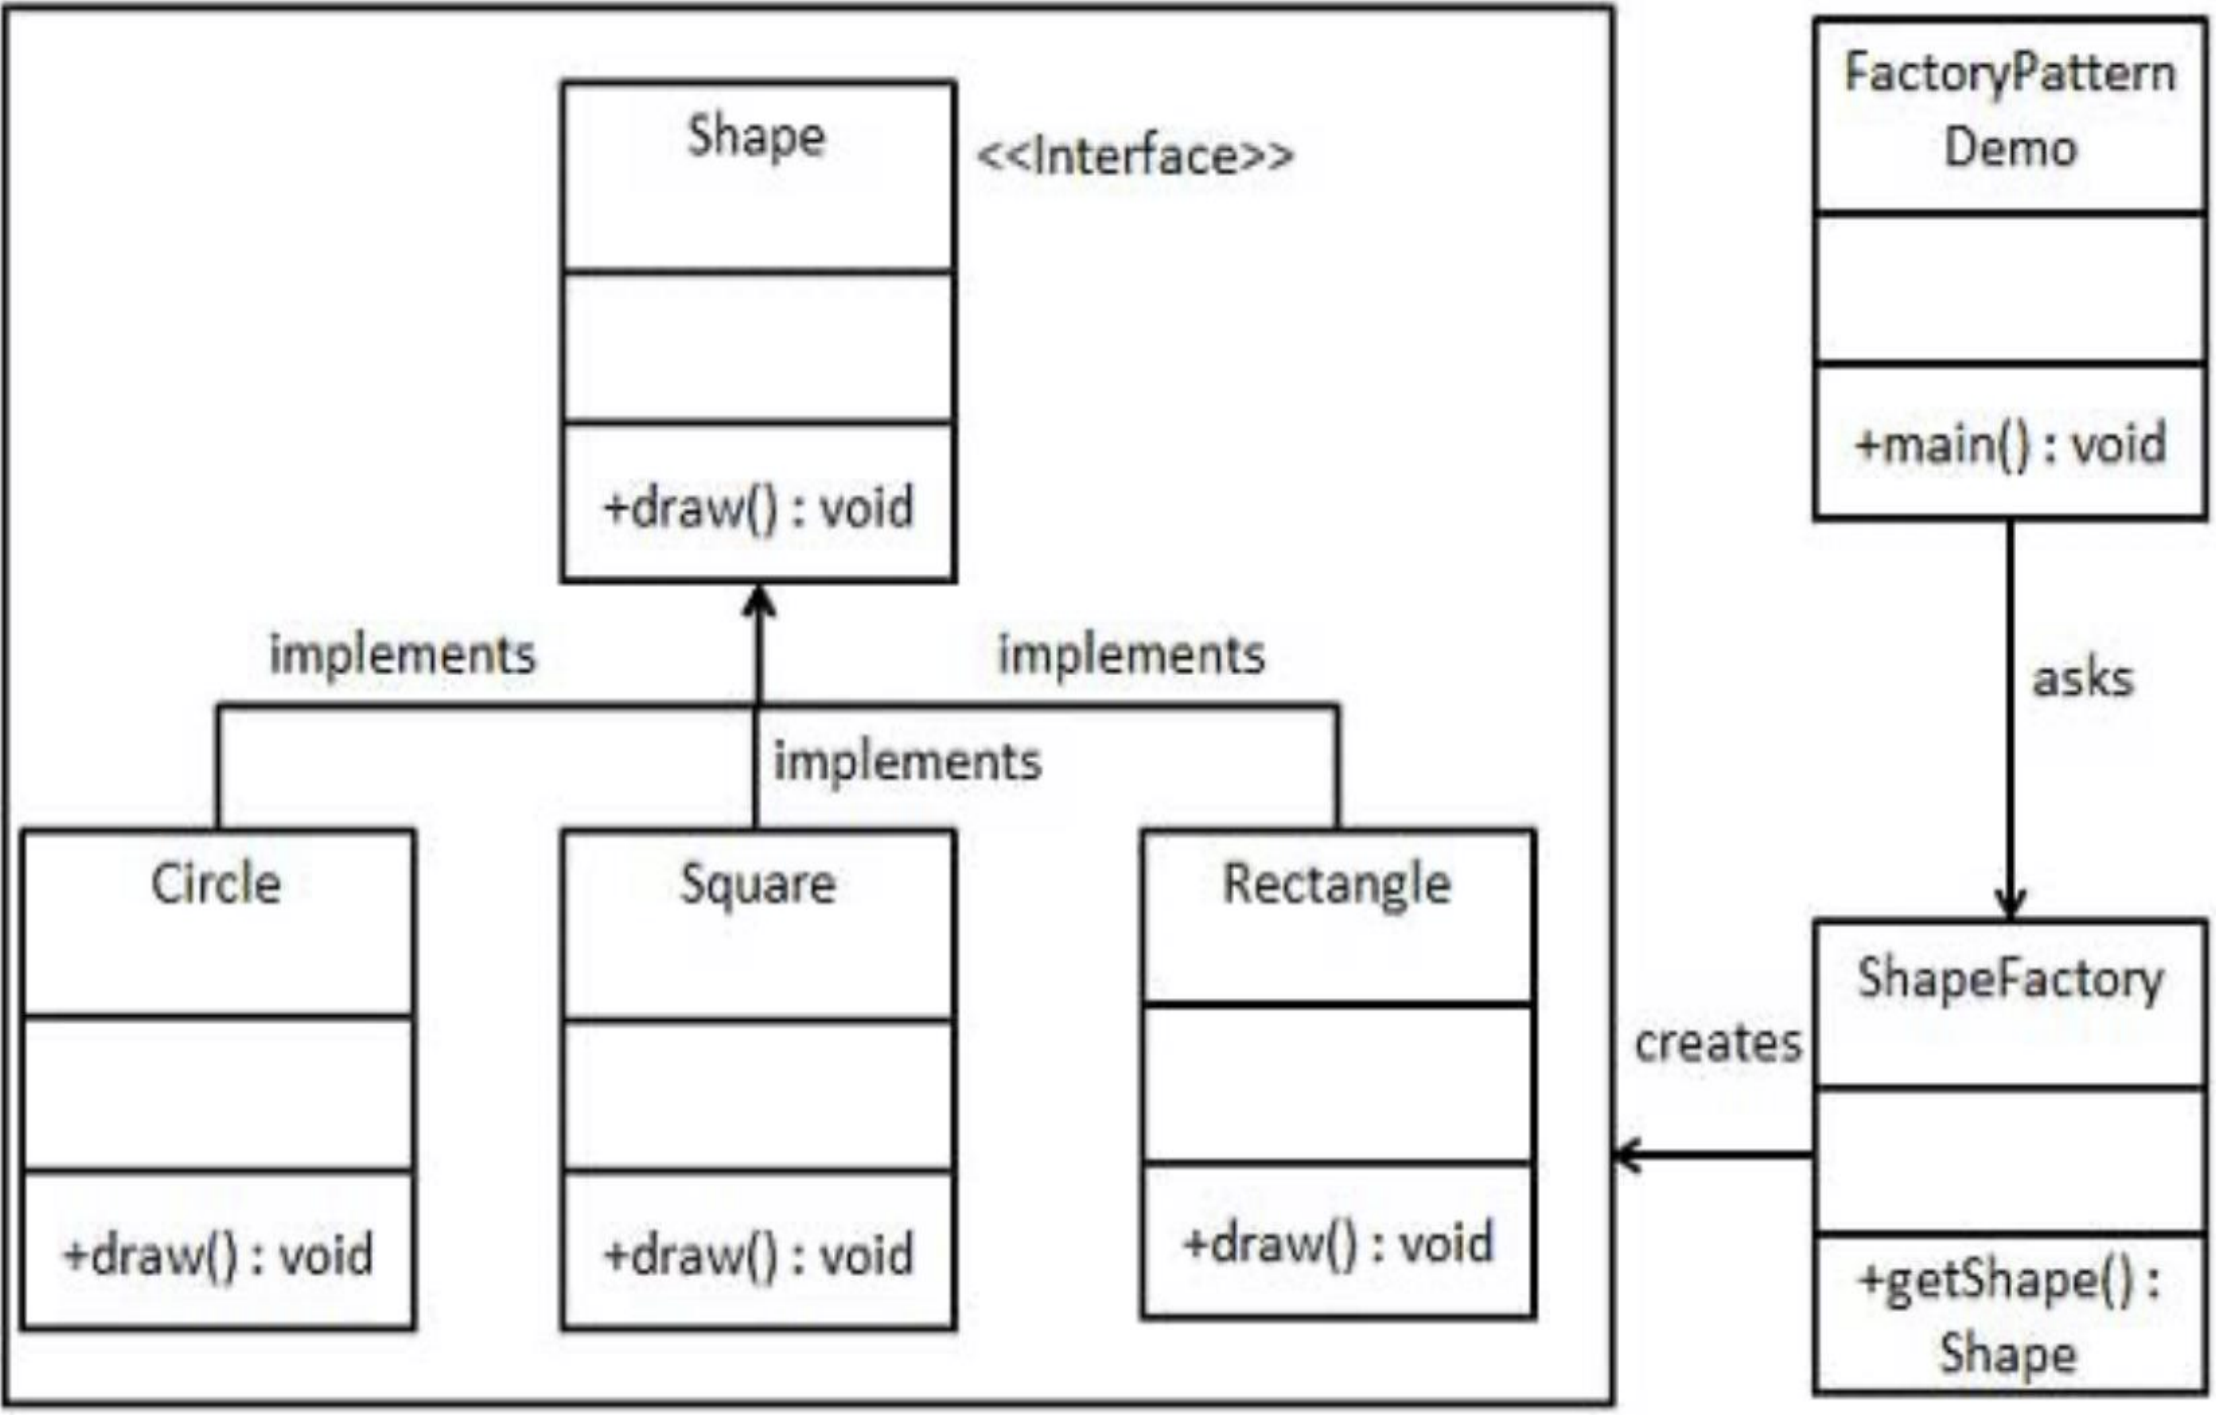
\includegraphics[width=0.35\textwidth]{shapesFactory.png}
        \end{center}
    \end{figure}


\begin{lstlisting}[style=JavaDraculaWhite]
 interface Shape {
    public void draw();
}

class Rectangle implements Shape {
    @Override
    public void draw() {
        System.out.println("Drawing a Rectangle");
    }
}

class Square implements Shape {
    @Override
    public void draw() {
        System.out.println("Drawing a square");
    }
}

class Circle implements Shape {
    public void draw() {
        System.out.println("Drawing a Circle");
    }
}

class ShapeFactory {
    public static Shape getShape(ShapeNames name) {
        if (name == ShapeNames.RECTANGLE) {
            return new Rectangle();
        } else if (name == ShapeNames.SQUARE) {
            return new Square();
        } else if (name == ShapeNames.CIRCLE) {
            return new Circle();
        } else {
            return null;
        }
    }
}

enum ShapeNames {
    RECTANGLE, SQUARE, CIRCLE
}

public class FactoryPatternDemo {
    public static void main(String[] args) {
        ShapeFactory.getShape(ShapeNames.CIRCLE).draw();
        ShapeFactory.getShape(ShapeNames.RECTANGLE).draw();
    }
}    
\end{lstlisting}

        \section{Patron de méthode}
    
        \begin{Concept}{Patron de méthode}{}
            À travers ce patron, on \textcolor{myb}{définit le squelette} d'un algorithme dans une 
            opération en \textcolor{myb}{reportant} certaines étapes à des sous-classes ou 
            méthode auxiliaires. Le but est d'implémenter une partir \textcolor{myb}{inveariante} d'un 
            algorthme et de laisser les autres méthode implémenter le comportement 
            qui va varier. 
        \end{Concept}


        \begin{EExample}{Classe abstraite pour patron méthode}{}

\begin{lstlisting}[style=JavaDraculaWhite]
abstract class AbstractClass {
    public void templateMethod() {
        primitiveOperation1(); 
        primitiveOperation2();
    }

    protected abstract void primitiveOperation1(); 
    protected abstract void primitiveOperation1(); 
}       
\end{lstlisting}
        \end{EExample}

        D'autres classes qui \texttt{extend AbstractClass} pourront être créées 
        Ces classes pourront overide les \texttt{primitiveOperation1} et \texttt{primitiveOperation2}; 
        elles pourront ensuite appeler la méthode publique \texttt{templateMethod} qui offre 
        le patron de l'algorithme. 


        \begin{figure}[H]
            \begin{center}
                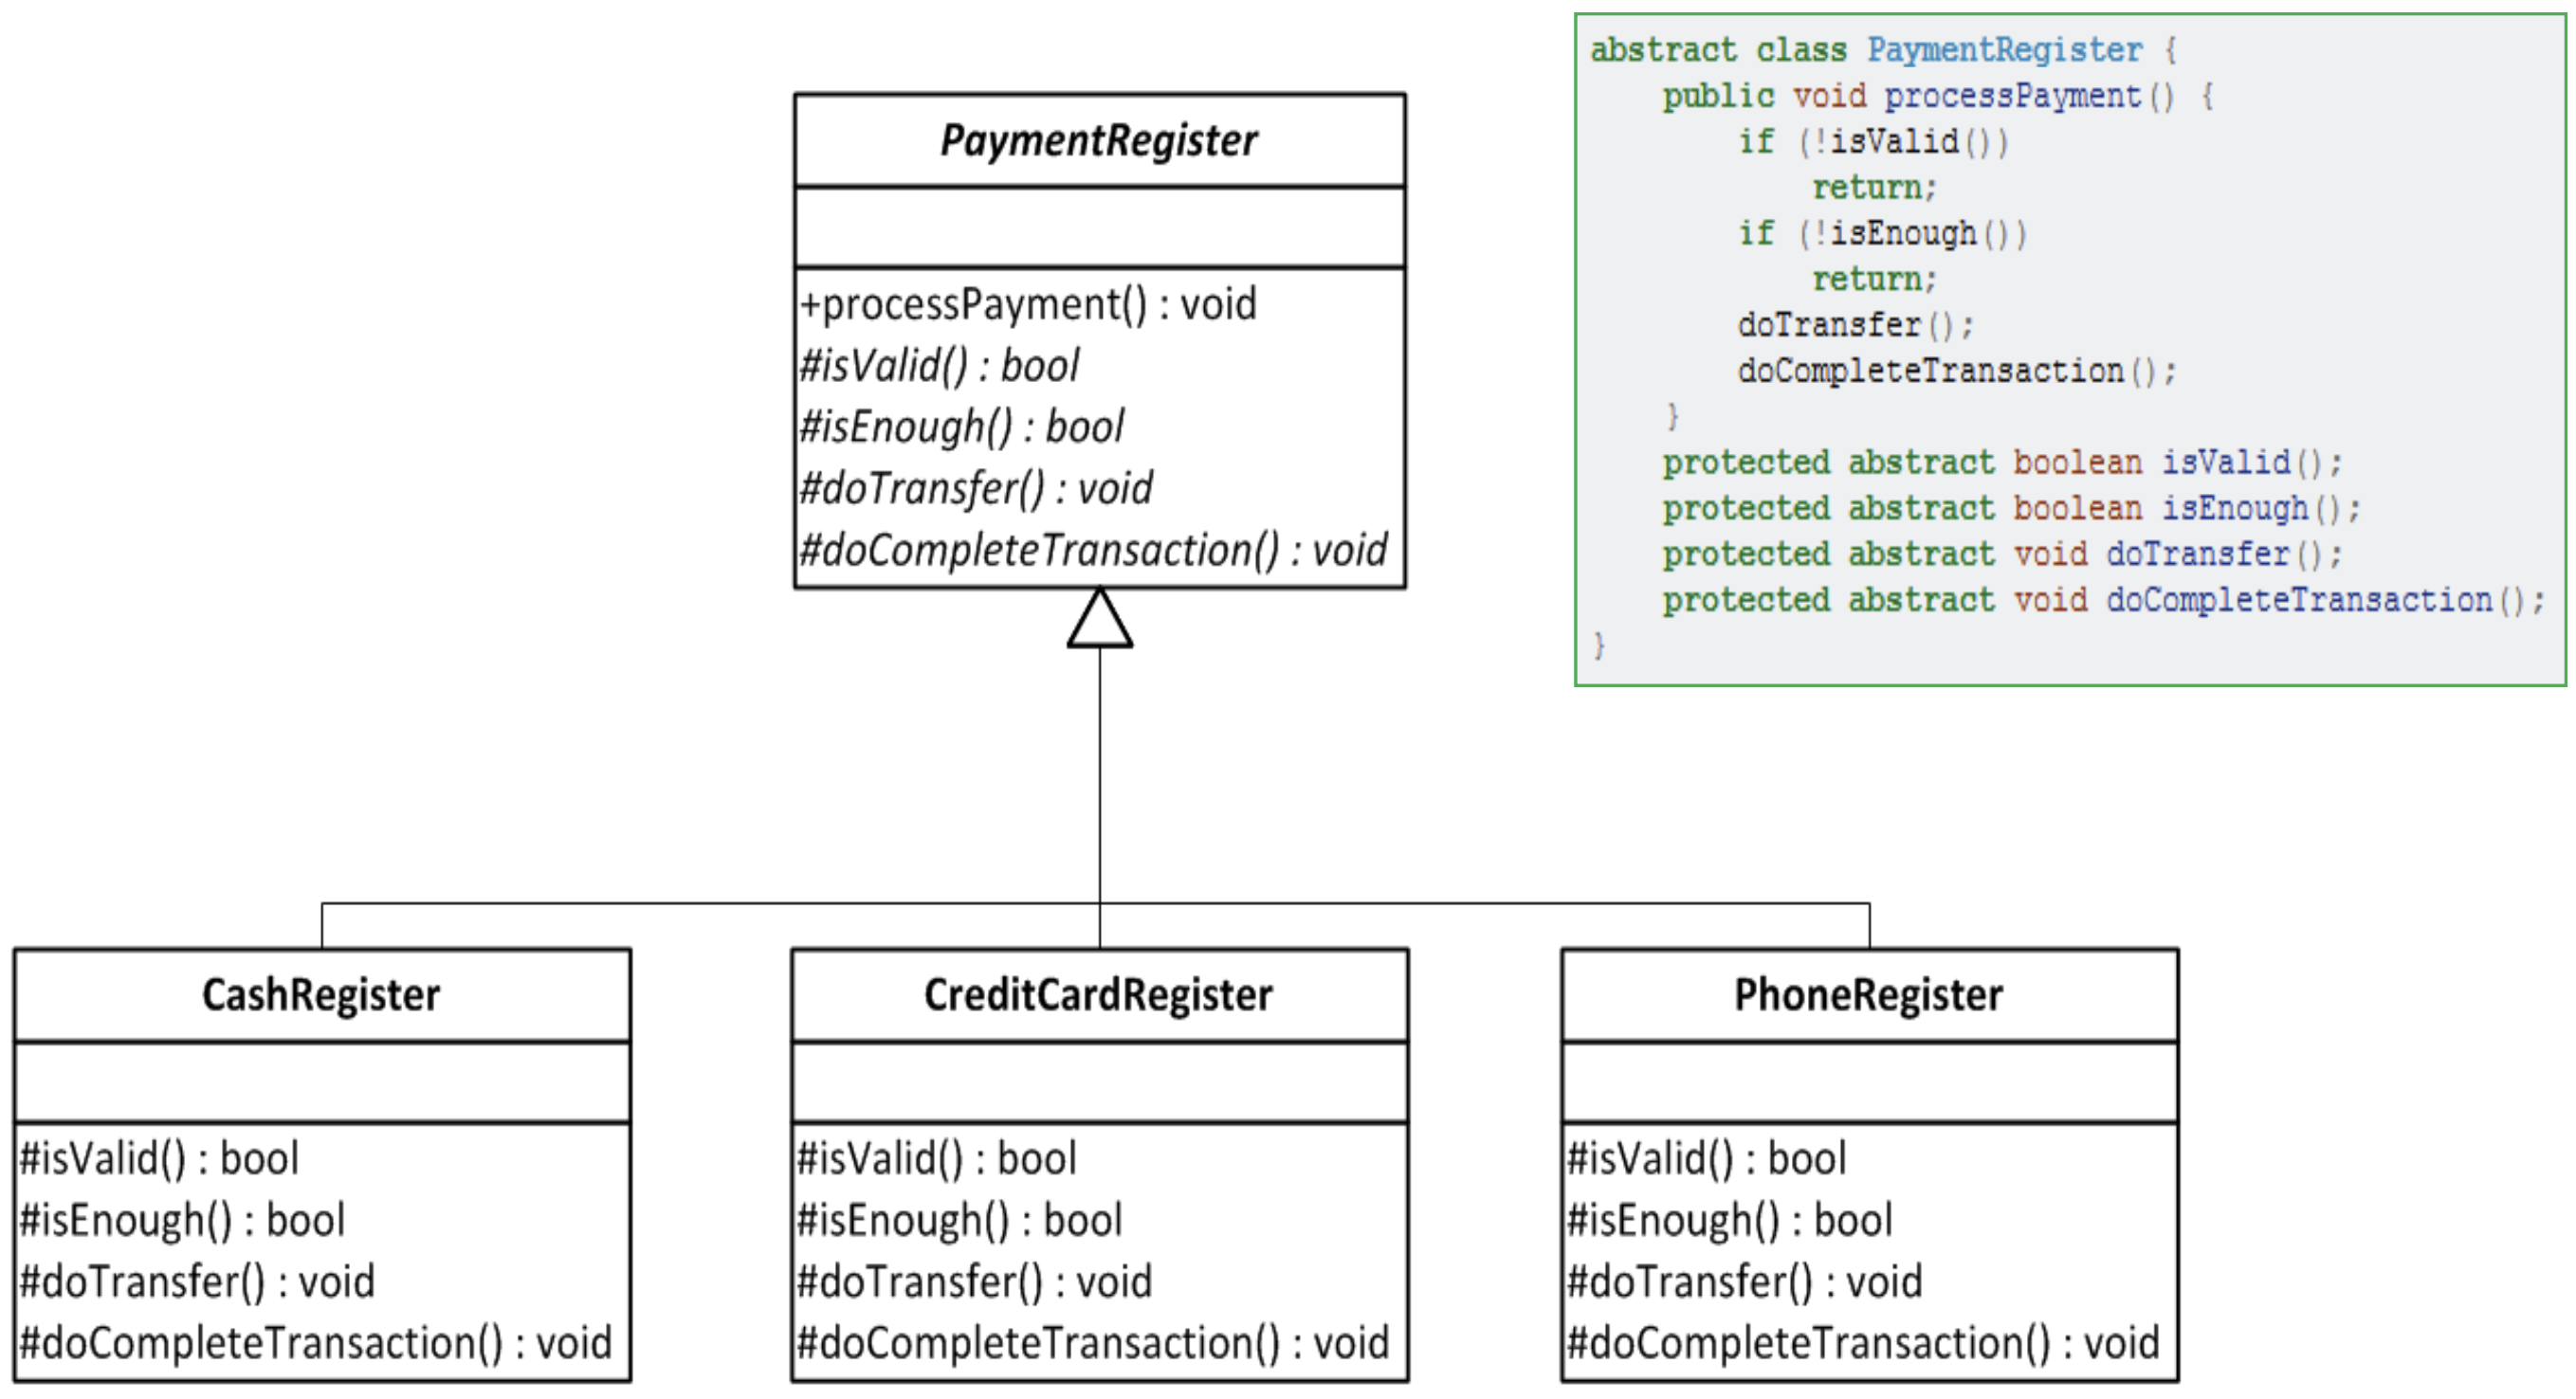
\includegraphics[width=0.40\textwidth]{patronMethode.png}
            \end{center}
        \end{figure}

        
        \section{Patron Stratégie}

        \begin{Concept}{Patron Stratégie}{}
            Le design patron Strategy est utile pour des situations où il est nécessaire de permuter
            dynamiquement les algorithmes utilisés dans une application (une solution lorsqu'un
            problème peut être résolu par différents algorithmes).
            Il définit une famille d'algorithmes encapsulés et interchangeables. Il encapsule des
            approches alternatives dans des classes distinctes qui implémentent chacune une
            opération commune.
            Les algorithmes peuvent être sélectionnés à la volée au cours du temps d'exécution
            selon certaines conditions
            
        \end{Concept}       


        \begin{figure}[H]
            \begin{center}
                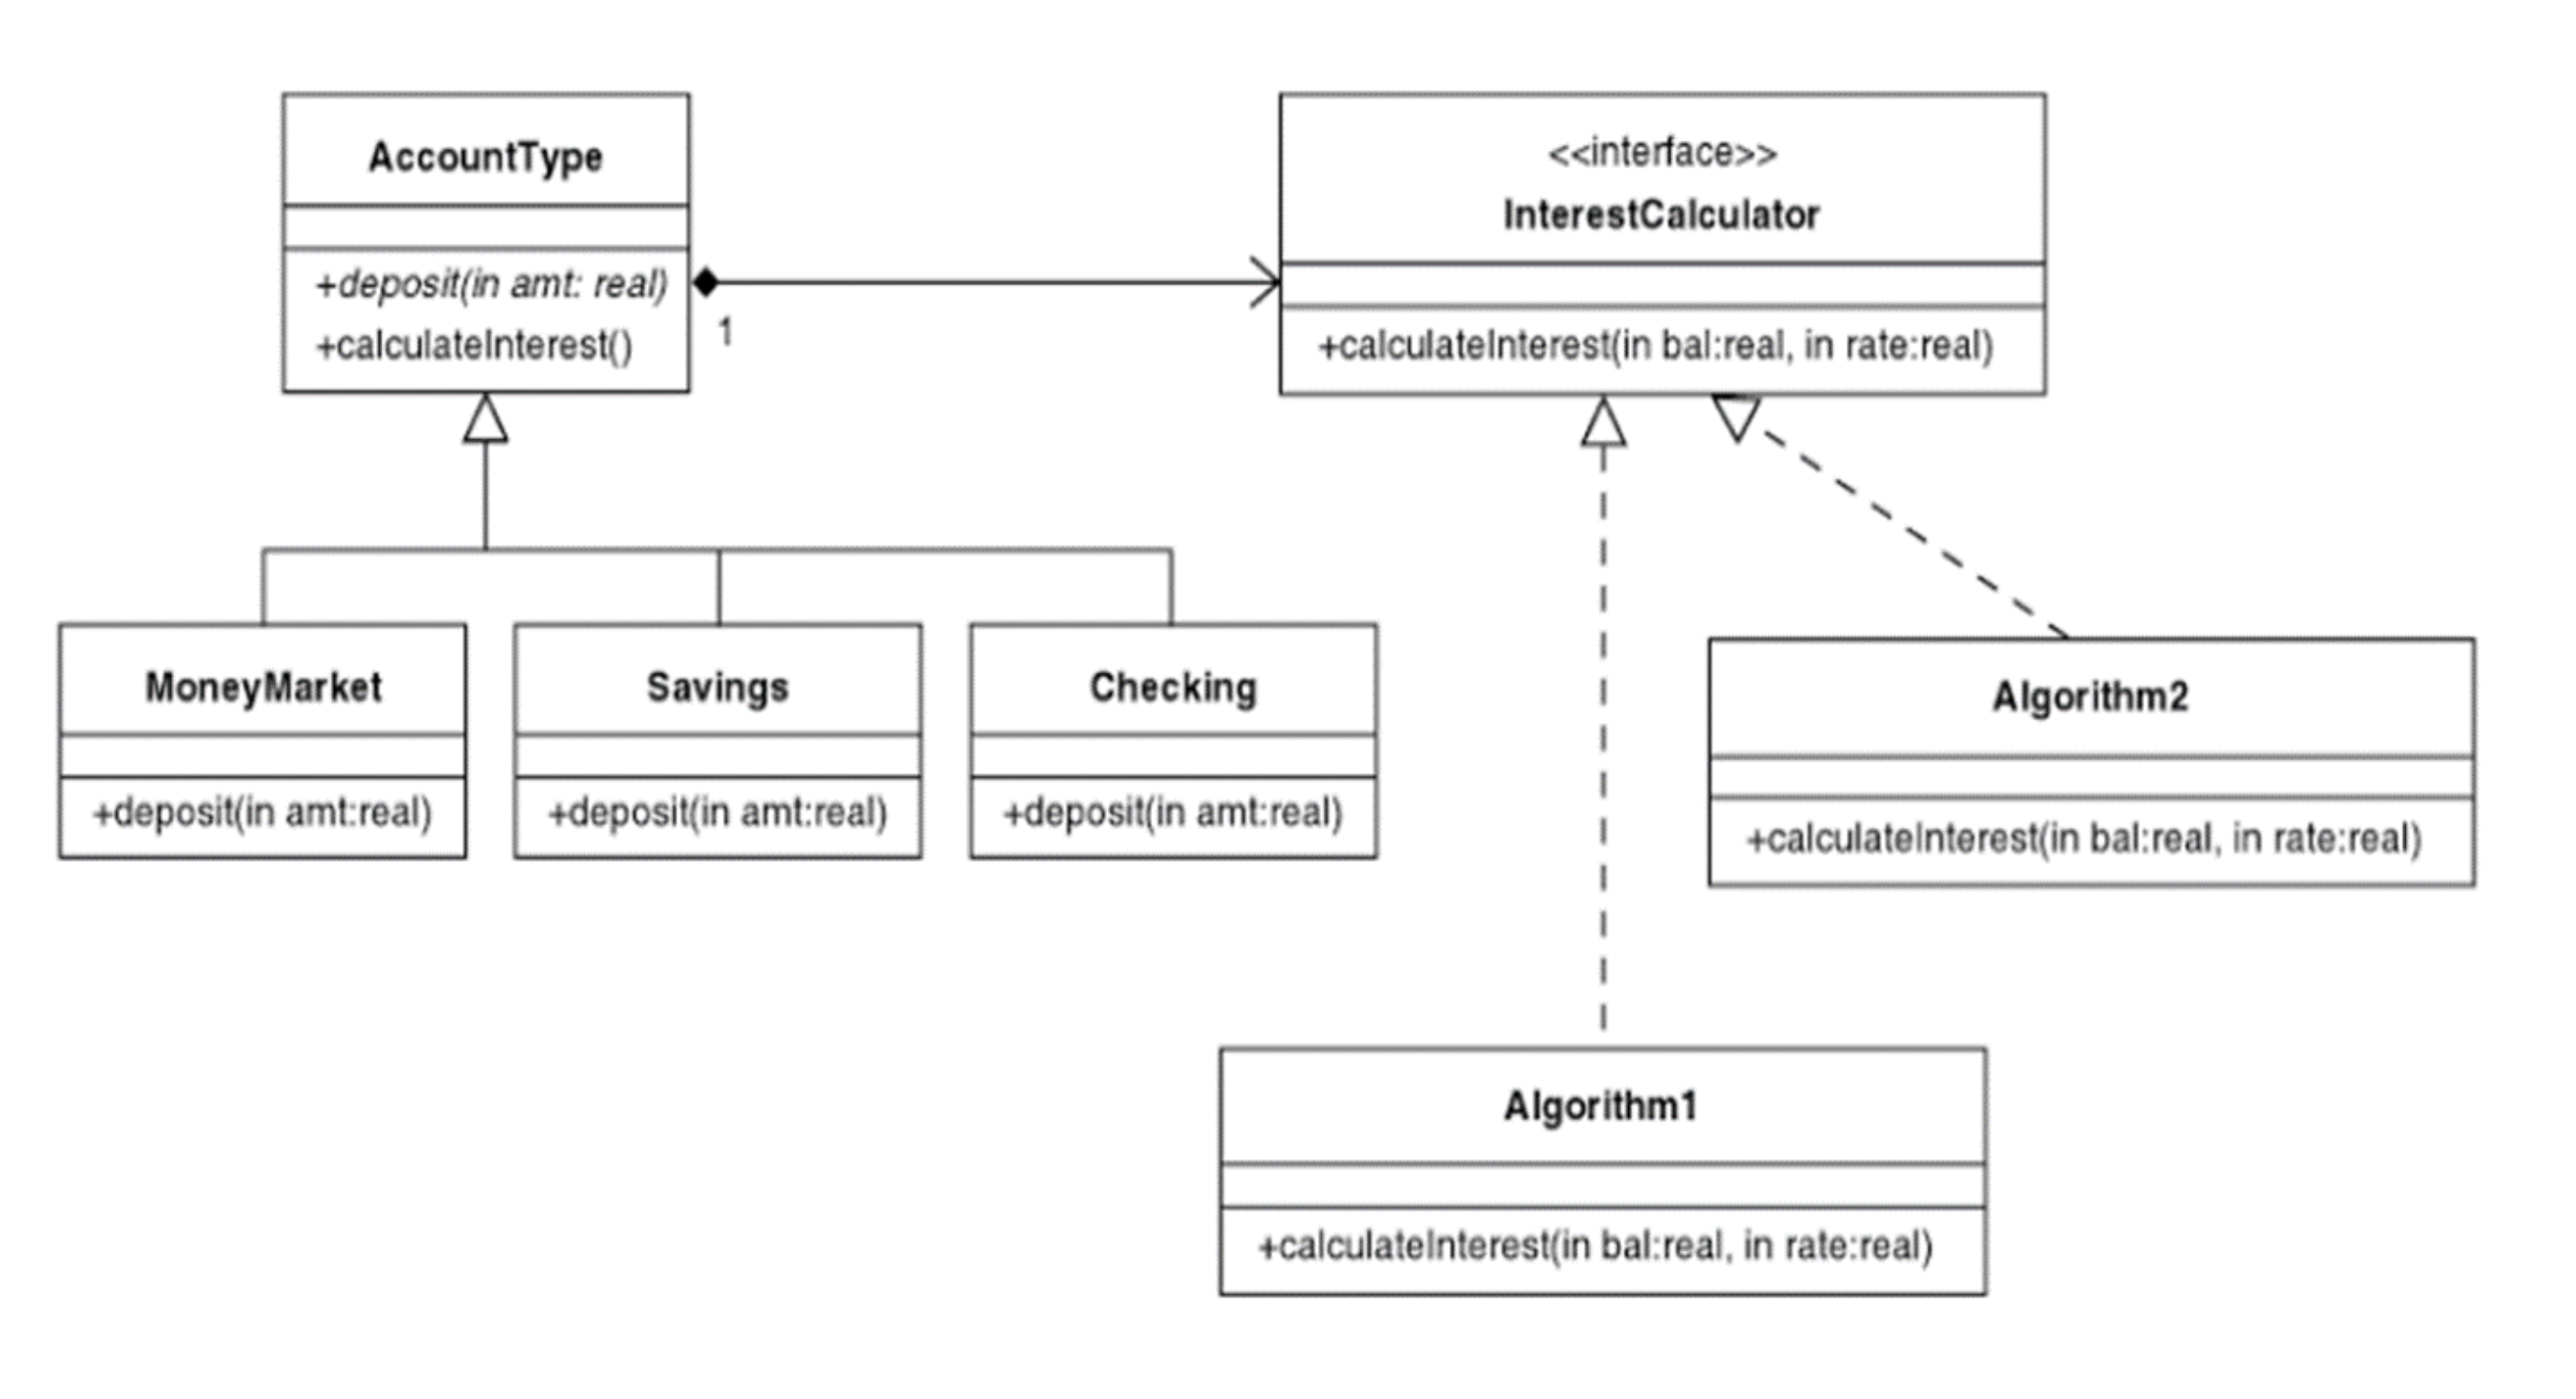
\includegraphics[width=0.40\textwidth]{PatronStrategy.png}
            \end{center}
        \end{figure}


        \begin{Concept}{Patron Decorator}{}
                Le patron Decorator ajoute dynamiquement des fonctionnalités supplémentaires
                à un objet.
                Un décorateur étend les responsabilités d'une classe en utilisant la composition et 
                non l'héritage. Un objet décorateur contient une instance d'objet d'origine en tant que variable
                membre et ajoute de nouvelles fonctionnalités avant ou/et après sa délégation à
                l'objet d'origine. Il relève du modèle de conception structurelle car il fournit l'un des meilleurs 
                moyens d'étendre les responsabilités d'une classe.
            
        \end{Concept}

\begin{lstlisting}[style=JavaDraculaWhite]
interface Computer {
    String getAllAccessories();
    int getCost();
}

class DefaultComputer implements Computer {
    public String getAllAccessories() {
        return "Default Computer";
    }

    public int getCost() {
        return 700;
    }
}

class ComputerDecorator implements Computer {
    Computer currentComputer;

    ComputerDecorator(Computer c) {
        currentComputer = c;
    }

    public String getAllAccessories() {
        return currentComputer.getAllAccessories();
    }

    public int getCost() {
        return currentComputer.getCost();
    }
}

class GPU extends ComputerDecorator {
    GPU(Computer c) {
        super(c);
    }

    public String getAllAccessories() {
        return super.getAllAccessories() +
        ", GeForce 3080 Ti GPU";
    }

    public int getCost() {
        return super.getCost() + 800;
    }
}

class Monitor extends ComputerDecorator {
    Monitor(Computer c) {
        super(c);
    }

    public String getAllAccessories() {
        return super.getAllAccessories() + ", Monitor";
    }

    public int getCost() {
        return super.getCost() + 500;
    }
}

\end{lstlisting}


        \section{Patron Builder}


        \begin{Concept}{Patron Builder}{}
            Le pattern Builder vous suggère d'extraire l'objet code
            de construction hors de sa propre classe et déplacez-le pour
            séparer objets appelés builders
        \end{Concept}   


        \begin{figure}[H]
            \begin{center}
                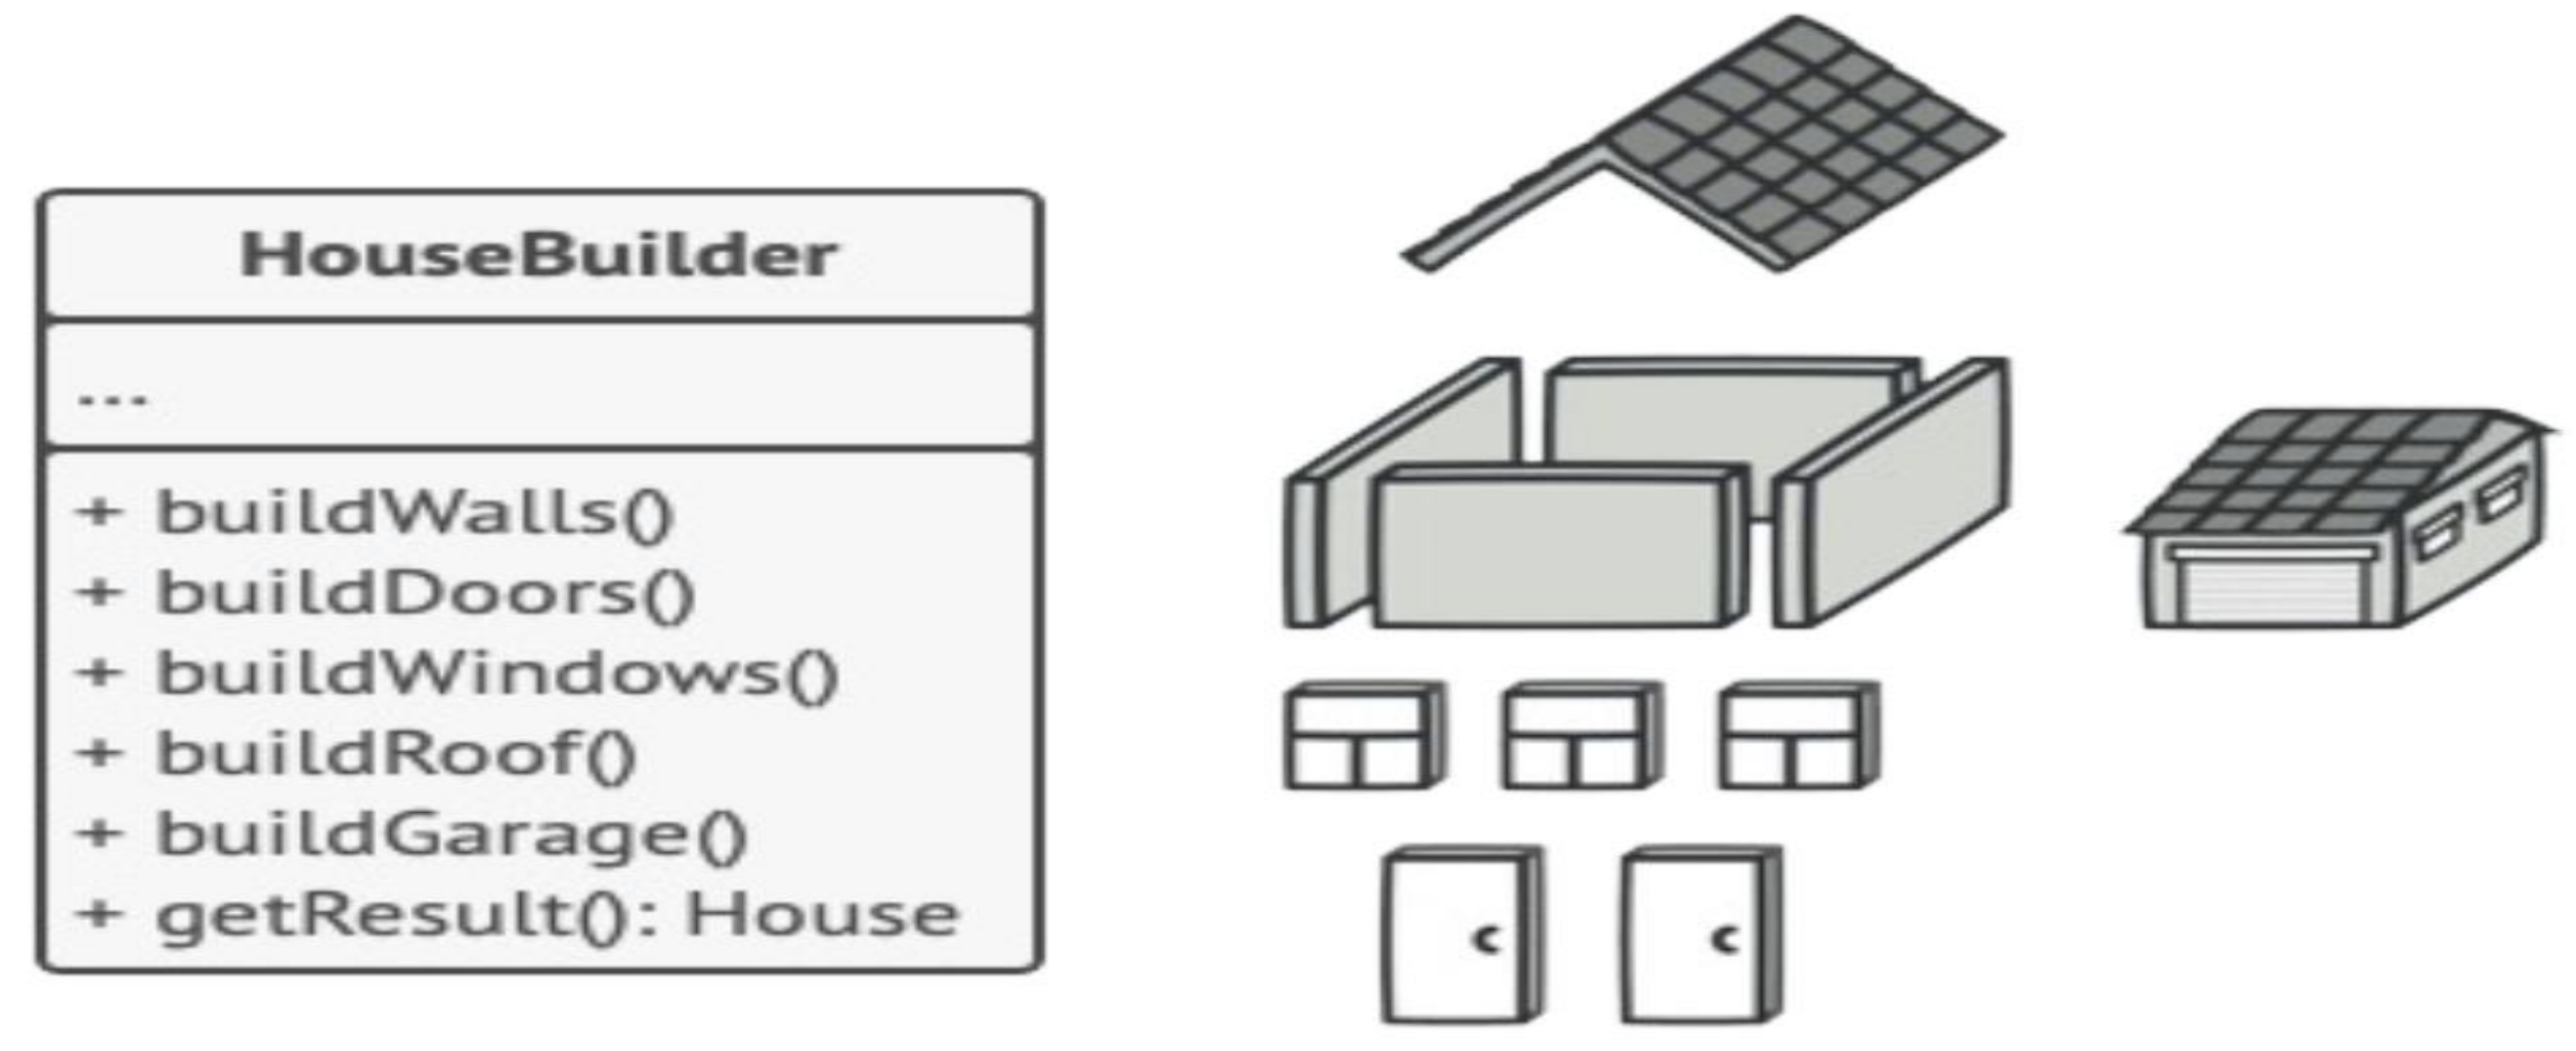
\includegraphics[width=0.40\textwidth]{PatronBuilder.png}
            \end{center}
        \end{figure}


\begin{lstlisting}[style=JavaDraculaWhite]
public static class Builder {
    private String engine;
    private int wheel;
    private int airbags;
    private boolean isAC = false;
    private boolean hasSunRoof = false;

    public Builder(String engine, int wheel) {
        this.engine = engine;
        this.wheel = wheel;
    }

    public Builder setAirbags(int num) {
        airbags = num;
        return this;
    }

    public Builder hasAC(boolean input) {
        isAC = input;
        return this;
    }

    public Builder hasSunRoof(boolean input) {
        hasSunRoof = input;
        return this;
    }

    public VehicleDirector build() {
        return new VehicleDirector(this);
    }
}

class VehicleDirector {
    private String engine;
    private int wheel;
    private int airbags;

    public String getEngine() { return this.engine; }
    public int getWheel() { return this.wheel; }
    public int getAirbags() { return this.airbags; }

    private VehicleDirector(Builder builder) {
        this.engine = builder.engine;
        this.wheel = builder.wheel;
        this.airbags = builder.airbags;
    }
}

public class BuilderDemo {
    public static void main(String[] args) {
        VehicleDirector v1 = 
        new VehicleDirector.Builder("1000cc", 4).build();
        System.out.println(v1);

        VehicleDirector v2 = 
        new VehicleDirector.Builder("500cc", 4)
                                .setAirbags(4)
                                .hasAC(true)
                                .hasSunRoof(false)
                                .build();
        System.out.println(v2);
    }
}
\end{lstlisting}
        
    \section{Patron Observer}

    \begin{Concept}{Patron Obvserver}{}
        Observer permet à un objet de demander à être notifié lorsqu’un autre
        objet change. \texttt{Observer} suppose que l’objet contenant les données 
        \textbf{est séparé} des objets affichant ces données. Les données sont le 
        \textcolor{myb}{sujet}. Les objets \textbf{afficheurs} sont les \textcolor{myb}{observateurs}. 
        Chaque observateur a une interface connue que le sujet appelle quand les données changent. 
        Toute entité appelée à être un sujet devra implémenter Sujet. 
        Toute entité appelée à être un observateur devra implémenter Observateur.
    \end{Concept}       


    \begin{EExample}{Exemple d'abonnement à un magazine}{}

\begin{lstlisting}[style=JavaDraculaWhite]
package ObserverPattern;

public class LocationTracker implements Observer {
    private int currentX, currentY;
  
    public void update(int xCordinate, int yCordinate){
 this.currentX = xCordinate;
 this.currentY = yCordinate;
 System.out.println("Current location of publisher is (" + currentX +
            ", " + currentY + ")");
    }
}

package ObserverPattern;

import java.util.ArrayList;

public class LocationTransponder implements Publisher {
    private int xCordinate, yCordinate;
    private ArrayList<Observer> observerList;
  
    public LocationTransponder(){
        observerList = new ArrayList<Observer>();
    }
  
    public void addObserver(Observer o){
        observerList.add(o);
    }
  
    public void removeObserver(Observer o){
        observerList.remove(o);
    }
  
    public void notifyObservers(){
        for(Observer o: observerList){
            o.update(xCordinate, yCordinate);
        }
    }
  
    public void setLocation(int x, int y){
       this.xCordinate = x;
       this.yCordinate = y;
       notifyObservers();
    }
}

package ObserverPattern;

public interface Observer {
    public void update(int xCordinate, int yCordinate);
}


package ObserverPattern;

public class PathDrawer implements Observer {
    private int currentX, currentY;
  
    public void update(int xCordinate, int yCordinate){
 if(currentX != xCordinate || currentY != yCordinate){
     System.out.println("Draw Line from  (" + currentX + ", " + currentY + 
      ") to (" + xCordinate + ", " + yCordinate + ")");
 } else {
     System.out.println("No Change in Position !!!!");
 }
 this.currentX = xCordinate;
 this.currentY = yCordinate;
    }
}

package ObserverPattern;

public interface Publisher {
    public void addObserver(Observer o);
    public void removeObserver(Observer o);
    public void notifyObservers();
}

public class ObserverPatternExample {
	
    public static void main(String args[]){
 LocationTransponder subject = 
 new LocationTransponder();
   
 Observer locationTracker = new LocationTracker();
 Observer pathDrawer = new PathDrawer();
   
 subject.addObserver(locationTracker);
 subject.addObserver(pathDrawer);
   
 // Changing state of the publisher(subject)
 subject.setLocation(2, 3);
 subject.setLocation(5, 10);
 subject.setLocation(5, 10);
    }
}

\end{lstlisting}
        
    \end{EExample}

    \section{Force des patrons de conceptions}

    \begin{itemize}
        \item Promeut la réutilisation en résolvant un problème de conception général
        \item Fournit une documentation de la conception en spécifiant des abstractions
        \item Lors de la maintenance, il est plus facile de comprendre un programme 
            qui utilise des patrons de conception, même sans avoir vu ce programme avant. 
    \end{itemize}

    \section{Faiblesse des patrons de conception}

    \begin{itemize}
        \item Pas de manière systématique de déterminer où et quand utiliser
            un patron deconception
        \item Programmes plus complexes emploient plusieurs patrons qui interagissent 
            entre eux pour maximiser leurs avantages (et leurs inconvénients…)
        \item Problème de gestion des dépendances entre patrons peut être 
            très complexe etperdre leurs avantages
        \item Le fait qu’on ait besoin de 23+ patrons de conception peut indiquer que notre 
            langage/paradigme n’est pas assez puissant, ou trop générique


    \end{itemize}
        

    \chapter{Implémentation}

    \begin{Definitionx}{Implémentation}{}
        Processus de traduction de la conception détaillé en code exécutable par une machine. 
    \end{Definitionx}
    \pagebreak


    \begin{note}{}{}
        Une \textbf{bonne conception} est rigoureuse (satisfaction des exigences), modulaire, 
        possède des mécanisme d'abstraction, permet l'adaptation aux changements, et généralise certains 
        de ses composnts pour qu'ils puissent être réutilisés à travers le système. 
    \end{note}

    Une \textbf{mauvaise conception}  présente des oublis de fonctionalités, engendre des conflits 
    entre les développeurs et rend certaines de leurs tâches redondantes, manque d'anticipation au 
    changement, engendre divers problèmes au niveau du code; ralentissement, duplication, gaspillage de ressources, 
    etc. 

    \section{Flux d'implémentation}

    \begin{itemize}
        \item \textbf{Partition du système en sous-système}  
        \item Implémentation d'artéfact par différents développeurs en parallèle 
        \item Test de l'artéfact 
        \item \textbf{Évaluation par l'équipe d'assurance qualité}  
    \end{itemize}

    \begin{note}{}{}
        Chaque artéfact est \textbf{testé après son implémentation}; celle-ci n'est pas considérée comme 
        complète tant que l'artéfact n'a été testé. 
    \end{note}                          
            
    \section{Tâches d'implémentation}

    \begin{itemize}
        \item Choisir le language 
        \item Établir les normes de programmation 
        \item Répartir l'effort de travail 
        \item Ingérer
    \end{itemize}

    \begin{note}{}{}
        La \textbf{répartition de l'effort} est indispensable. Il faut \textcolor{myb}{assigner} différents 
        modules à différents développeurs. Il faut \textbf{gérer les changements d'assignation} 
        en cas de maladie, démission, recrue, ajustement de temps, etc. 
    \end{note}

    \begin{itemize}
        \item \textbf{Choix du langage de programmation}  
        \begin{itemize}
            \item[$\blacktriangleright$] Pas toujours libre de choix 
            \item[$\blacktriangleright$] Généralement spécifié par le contrat
            \item[$\blacktriangleright$] L'environnement de développement peut également restreindre le choix 
            \item[$\blacktriangleright$] Il faut considérer les préférences de l'équipe de dév. 
        \end{itemize}
    \end{itemize}

    \section{Diversité des langages de programmation}


    \begin{itemize}
        \item \textbf{Évolution empirique}  
            \begin{itemize}
                \item[$\blacktriangleright$] Remplacement des instructions \texttt{GOTO} par des 
                    \texttt{While} et \texttt{Case} dans les années 1970.     
                \item[$\blacktriangleright$] Adoption de l'OOP grâce à l'avènement de l'imbrication de code 
                    dans les années 1980.
            \end{itemize}
        \item \textbf{Besoin spécifiques}  
            \begin{itemize}
                \item[$\blacktriangleright$] Plusieurs langage ont été conçus pour des besoin spécifiques 
            \end{itemize}
        \item \textbf{Préférences personnelles}  
    \end{itemize}

        \section{Bonnes pratiques de programmation}

    \begin{figure}[H]
        \begin{center}
            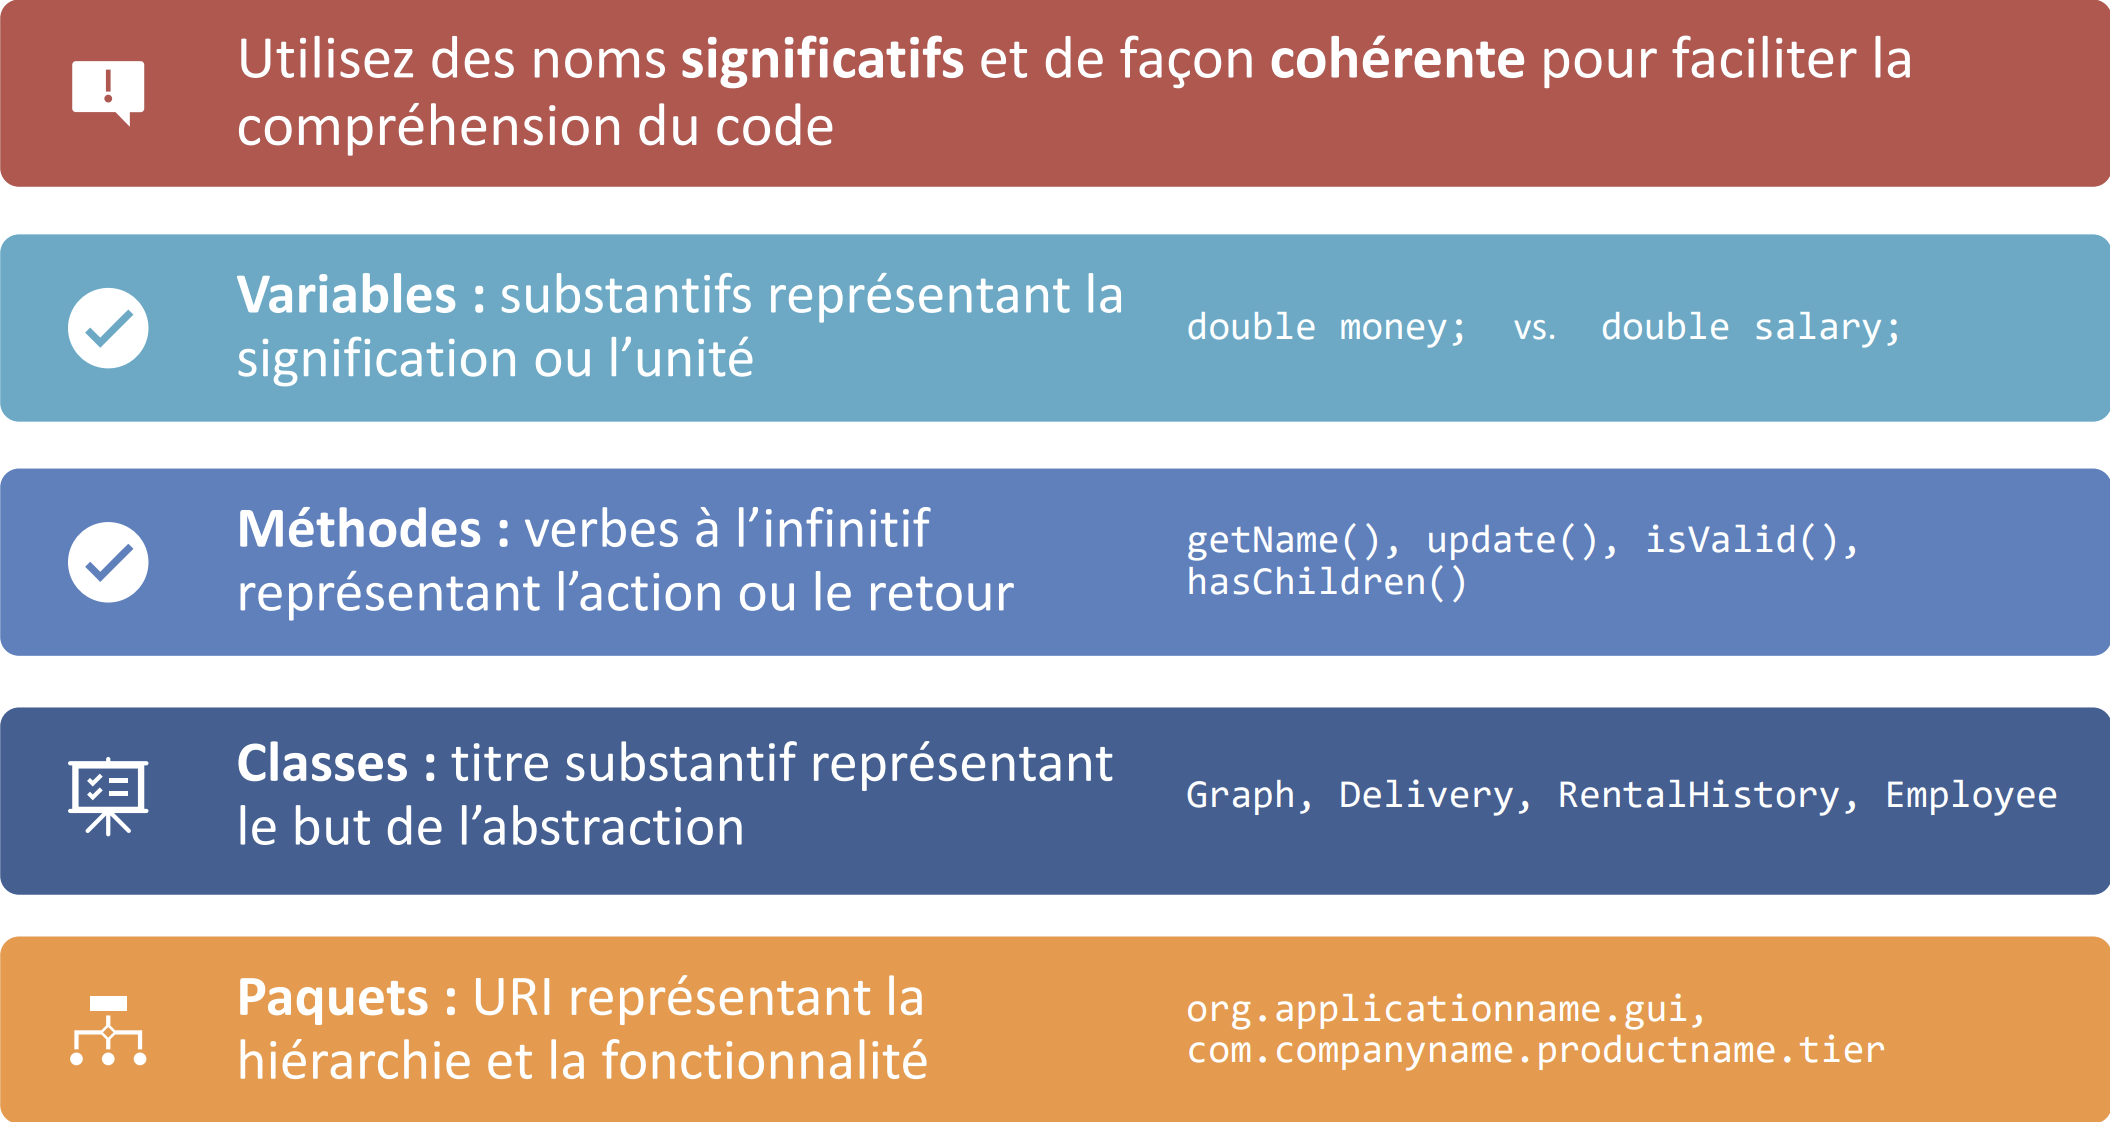
\includegraphics[width=0.45\textwidth]{BonnesPraiquesProg.png}
        \end{center}
    \end{figure}


    \begin{itemize}
        \item \textbf{Éviter les ambiguités}  
            \begin{itemize}
                \item[$\blacktriangleright$] \texttt{freqAvarage}, \texttt{fraquencyMaximum}, \texttt{minFr}, 
                    \texttt{frqncyTotl} 
                \item[$\rhd$] Est-ce que ces trois variables référence à la même chose (fréquence) ?
                \item[$\rhd$] Si oui, utiliser le même mot 
                \item[$\rhd$] \texttt{frequencyAverage}, 
                    \texttt{frequencyMaximum}
                \item[$\rhd$] \texttt{frequencyMinimum}, \texttt{frequencyTotal}  
            \end{itemize}
    \end{itemize}

    Éviter les \textbf{caractères faciles à confondre}, p. ex. 1 l L, o O 0, S, 5, G, 6, etc. Les 
    \textcolor{myb}{noms trompeurs} ou \textcolor{myb}{génériques} ayant plusieurs sens p. ex. 
    \texttt{money}, \texttt{date}, \texttt{bouton}, etc. Éviter les \textbf{synonymes} p. ex.  
    \texttt{average} \texttt{mean}. Utiliser les majuscules de façon cohériente et logique : p. ex. 
    \texttt{HelloWorld}.  


    \begin{itemize}
        \item \textbf{Espaces, ligne blanches}  
            \begin{itemize}
                \item[$\blacktriangleright$] Utiliser les espaces pour structurer en paragraphes
            \end{itemize}
        \item \textbf{Regroupement}  
            \begin{itemize}
                \item[$\blacktriangleright$] Rapprocher les méthodes qui collaborent. 
                \item[$\blacktriangleright$] Grouper par visibilité.
            \end{itemize}
        \item \textbf{Alignement, indentation, aération}
            \begin{itemize}
                \item[$\blacktriangleright$] Considérer la logique; boucles impliquées, contenant et contenu, etc.
            \end{itemize}
        \item \textbf{Parenthèse, accolades}
    \end{itemize}


    \begin{note}{}{}
        \textbf{Commenter les sections de code} qui ne sont pas évidentes est une bonne pratique.   
        Utiliser les commentaires partimonieusement. Il est préférable de 
        \textbf{recoder clairements} les portions trop complexes plutôt que d'abuser 
        de l'ambiguité et des commentaires. 
    \end{note}


    \section{Normes de programmation}

    Les difficultés surviennent souvent lorsque des normes arbitraires sont donées. P. ex. 
    \textit{Chaque module doit contenir entre 35 et 50 instructions exécutables}. Une meilleure norme 
    serait \textit{Le programmeur doit consulter sont supérieur avant de construire un module de moins de 
    35 ou de plus de 50 instructions exécutables}. Les normes devraient être vérifiables sans 
    interventions humaine. L'\textbf{objectif} des normes est de standardiser et de 
    \textit{rendre la maintenance facile}.  



    \begin{figure}[H]
        \begin{center}
            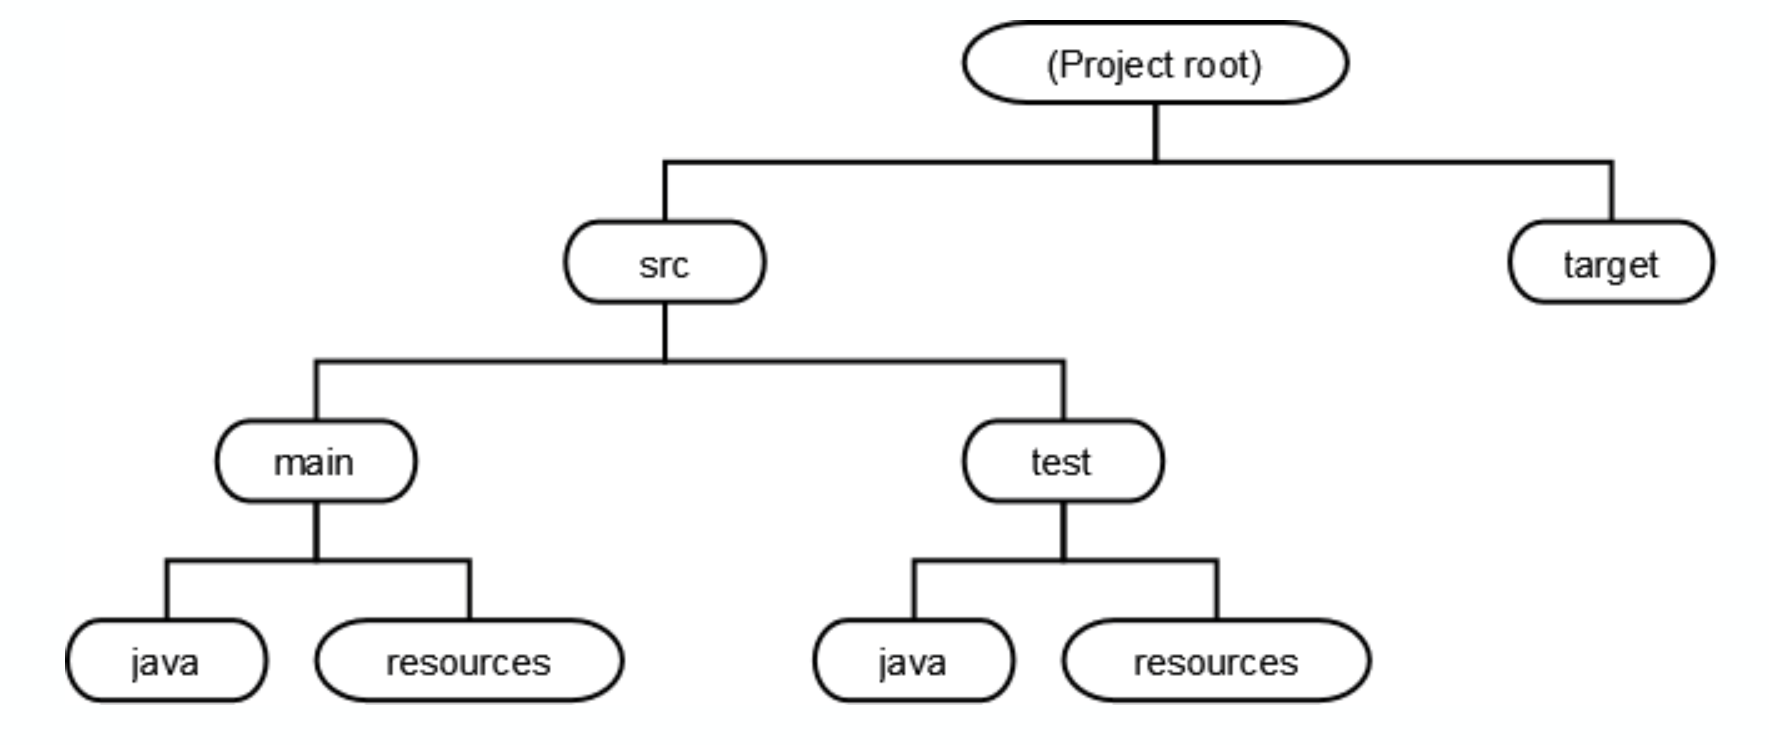
\includegraphics[width=0.45\textwidth]{ORganisation.png}
        \end{center}
    \end{figure}

    \section{Outils de programmation}


        Les développeurs utilisent différents outils durant la vie du logiciel
        p. ex. vérificateur d’interfaces, compilateur, éditeur texte, etc.
        Les outils peuvent être combiné dans un environnement qui apporte un support par
        ordinateur à plusieurs activités
        p. ex. programmation, test, contrôle de configuration, gestion de révisions, moteur de
        production, interpréteur, débogueur
        Une \textbf{IDE} intègre ces environnements et outils dans une interface utilisateur commune et
        uniforme : même présentation; outils communiquent avec des données compatibles.
        Idéalement, une IDE devrait intégrer tout le processus de développement


        \section{Débogage}

        \begin{itemize}
            \item \textbf{Bloqueur}  
                \begin{itemize}
                    \item[$\blacktriangleright$]  empêche de poursuivre les tests jusqu’à ce qu’il soit corrigé ou 
                        une alternative est identifiée
                \end{itemize}
            \item \textbf{Critique}
                \begin{itemize}
                    \item[$\blacktriangleright$] Impossible d'éviter la perturbation d'opérations essentielles; 
                        sécurité compromise
                \end{itemize}
            \item \textbf{Maheure}
                \begin{itemize}
                    \item[$\blacktriangleright$] Opération essentielle est affectée, mais on peut continuer 
                \end{itemize}
            \item \textbf{Mineur}
                \begin{itemize}
                    \item[$\blacktriangleright$] Opération non-essentielle est perturbée
                \end{itemize}
            \item \textbf{Inconséquent}
                \begin{itemize}
                    \item[$\blacktriangleright$] Pas d'impact significatif sur les opérations. 
                \end{itemize}
        \end{itemize}

        \begin{Definitionx}{Debogeur}{}
            Un \textbf{débogeur} simule l'exécution du code et permet d'examiner les erreurs rencontrées. 
            Il utilise les stratégie d'\textbf{exécution en étape} \texttt{step} et de \textbf{suspension}
            \texttt{break}.   
        \end{Definitionx}


        \begin{figure}[H]
            \begin{center}
                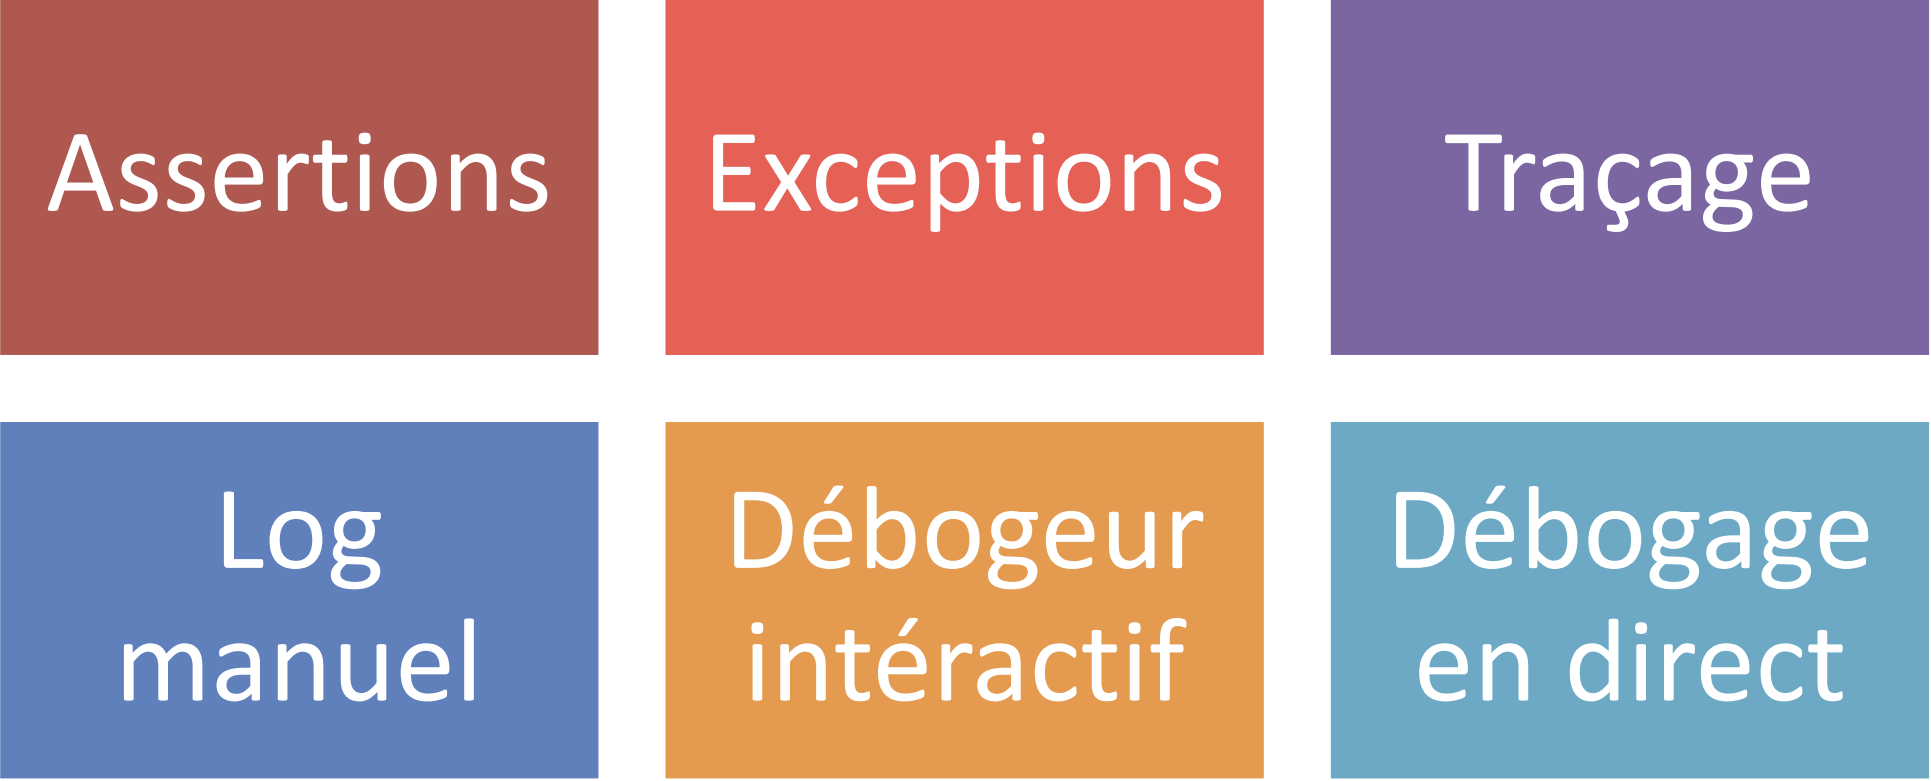
\includegraphics[width=0.15\textwidth]{MethodesDebogage.png}
            \end{center}
        \end{figure}


        \section{Cycle de vie d'un bogue}


        \begin{figure}[H]
            \begin{center}
                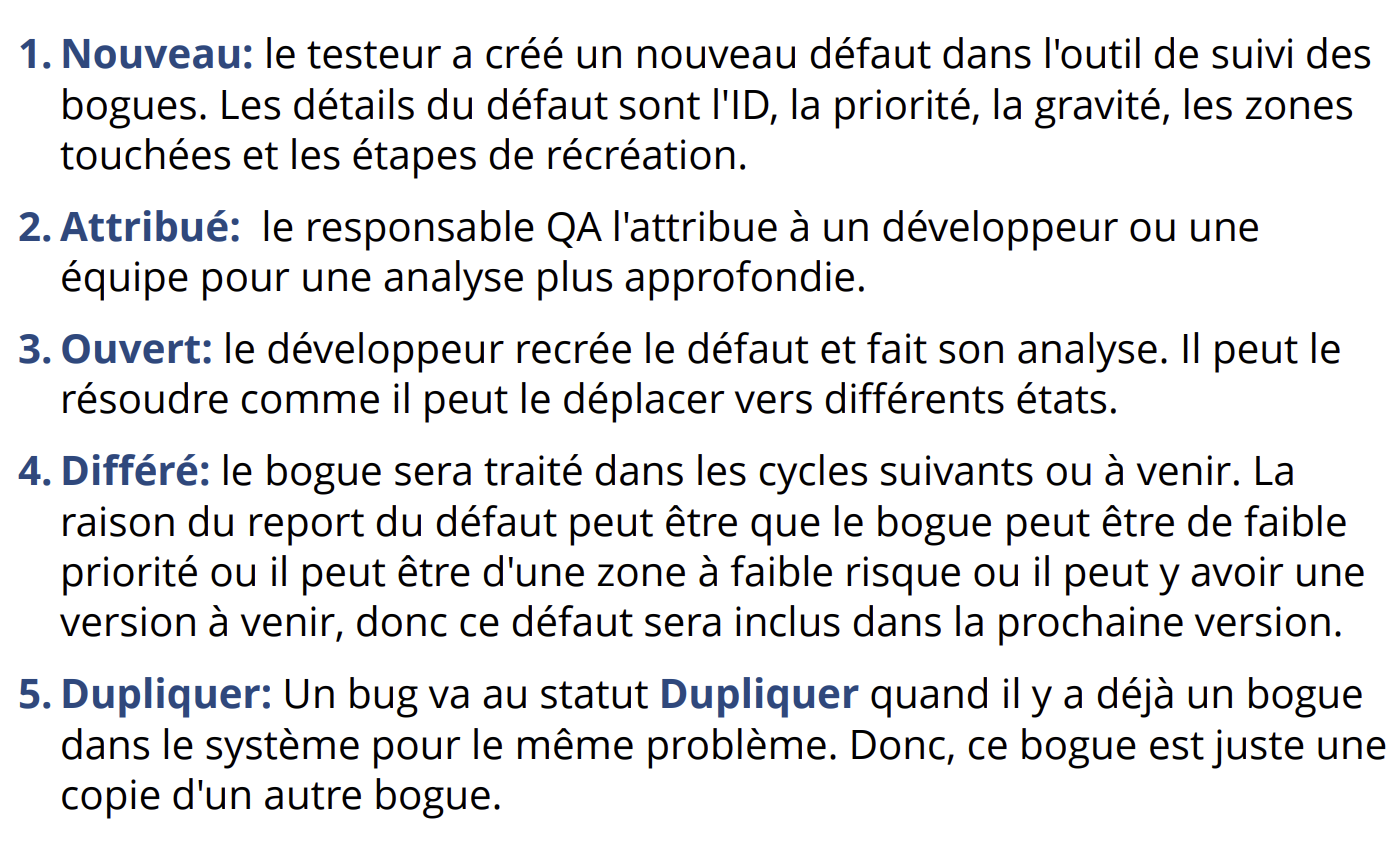
\includegraphics[width=0.42\textwidth]{cyclevie1.png}
            \end{center}
        \end{figure}
        

        \begin{figure}[H]
            \begin{center}
                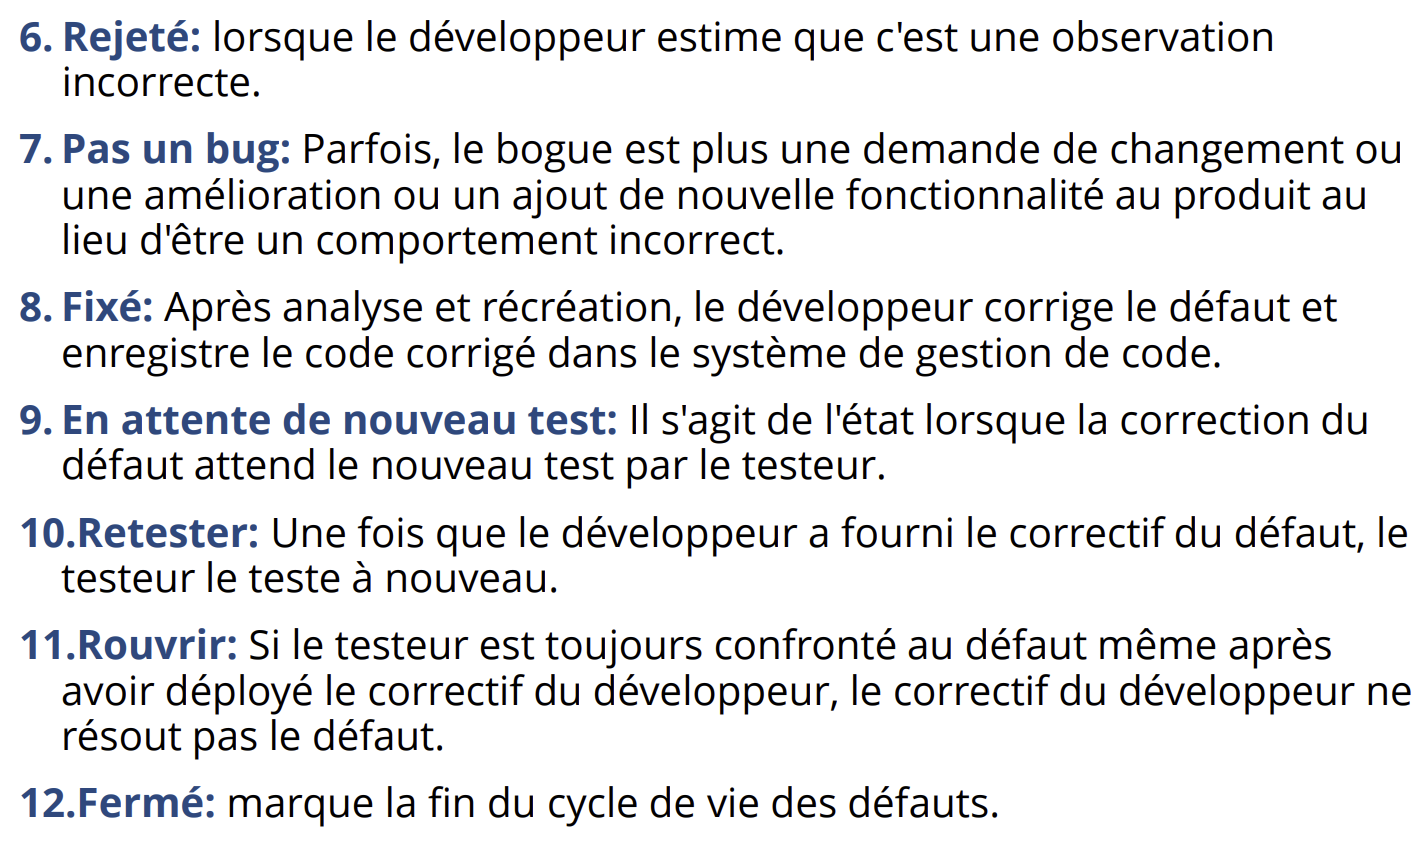
\includegraphics[width=0.42\textwidth]{cyclevie2.png}
            \end{center}
        \end{figure}


        \begin{figure}[H]
            \begin{center}
                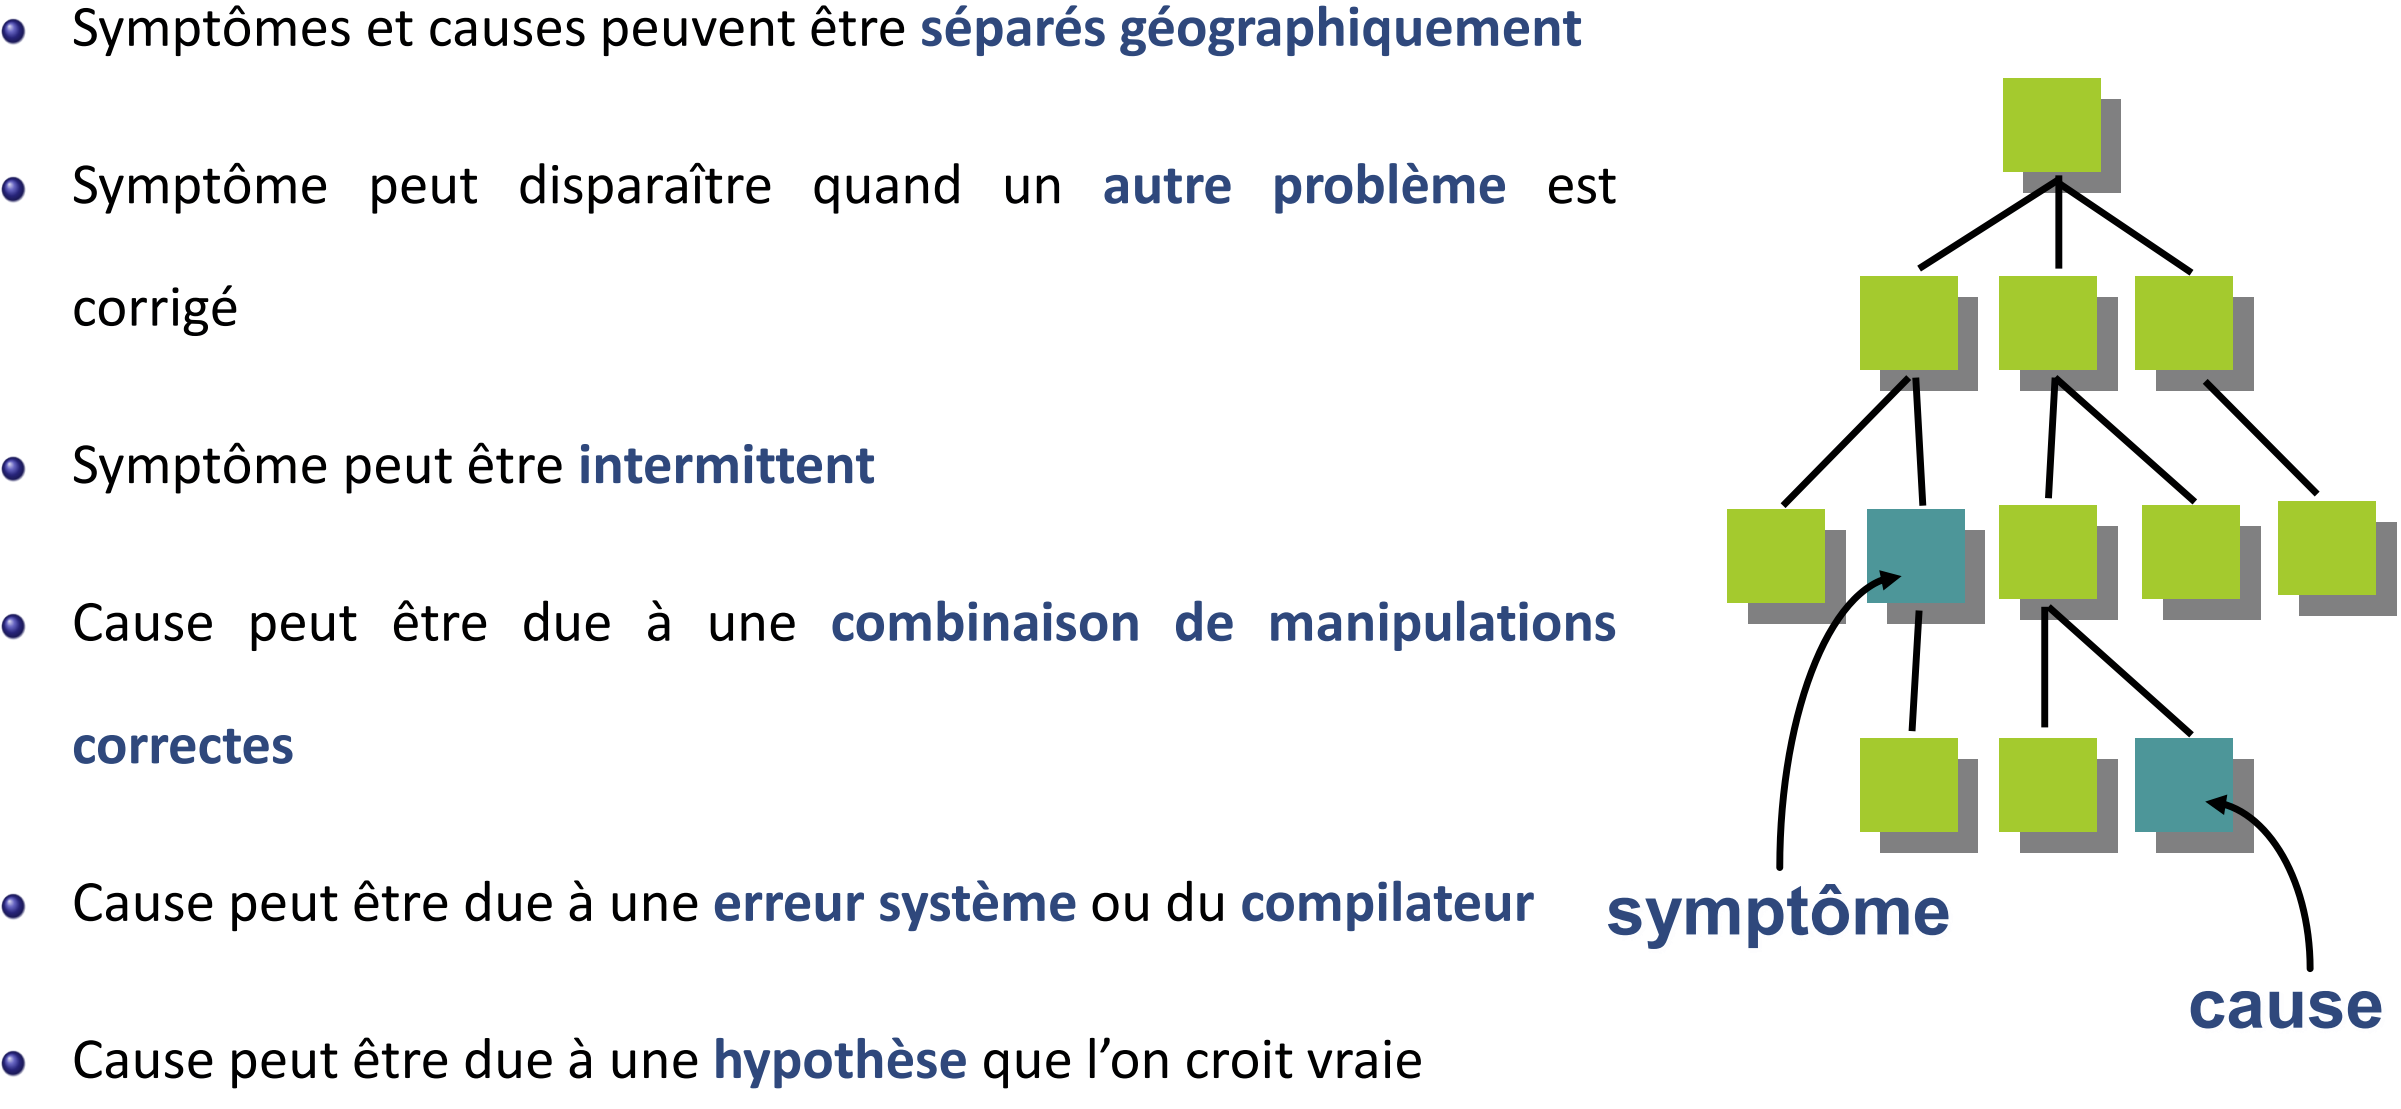
\includegraphics[width=0.50\textwidth]{symptCause.png}
            \end{center}
        \end{figure}


        \chapter{Vérification et validation \texttt{\S \; Amal 19}  }

        \begin{note}{}{}
            La \textbf{qualité d'un logociel} se mesure davantage par l'absence de défaut 
            plutôt que la présence d'éléments exceptionnels.
        \end{note}

        \section{Pertinence fonctionnelle}
        
        \begin{Concept}{Pertinence fonctionnelle}{}
            Mesure du lien entre la perfomance et le respect des exigences.
        \end{Concept}

        \begin{figure}[H]
            \begin{center}
                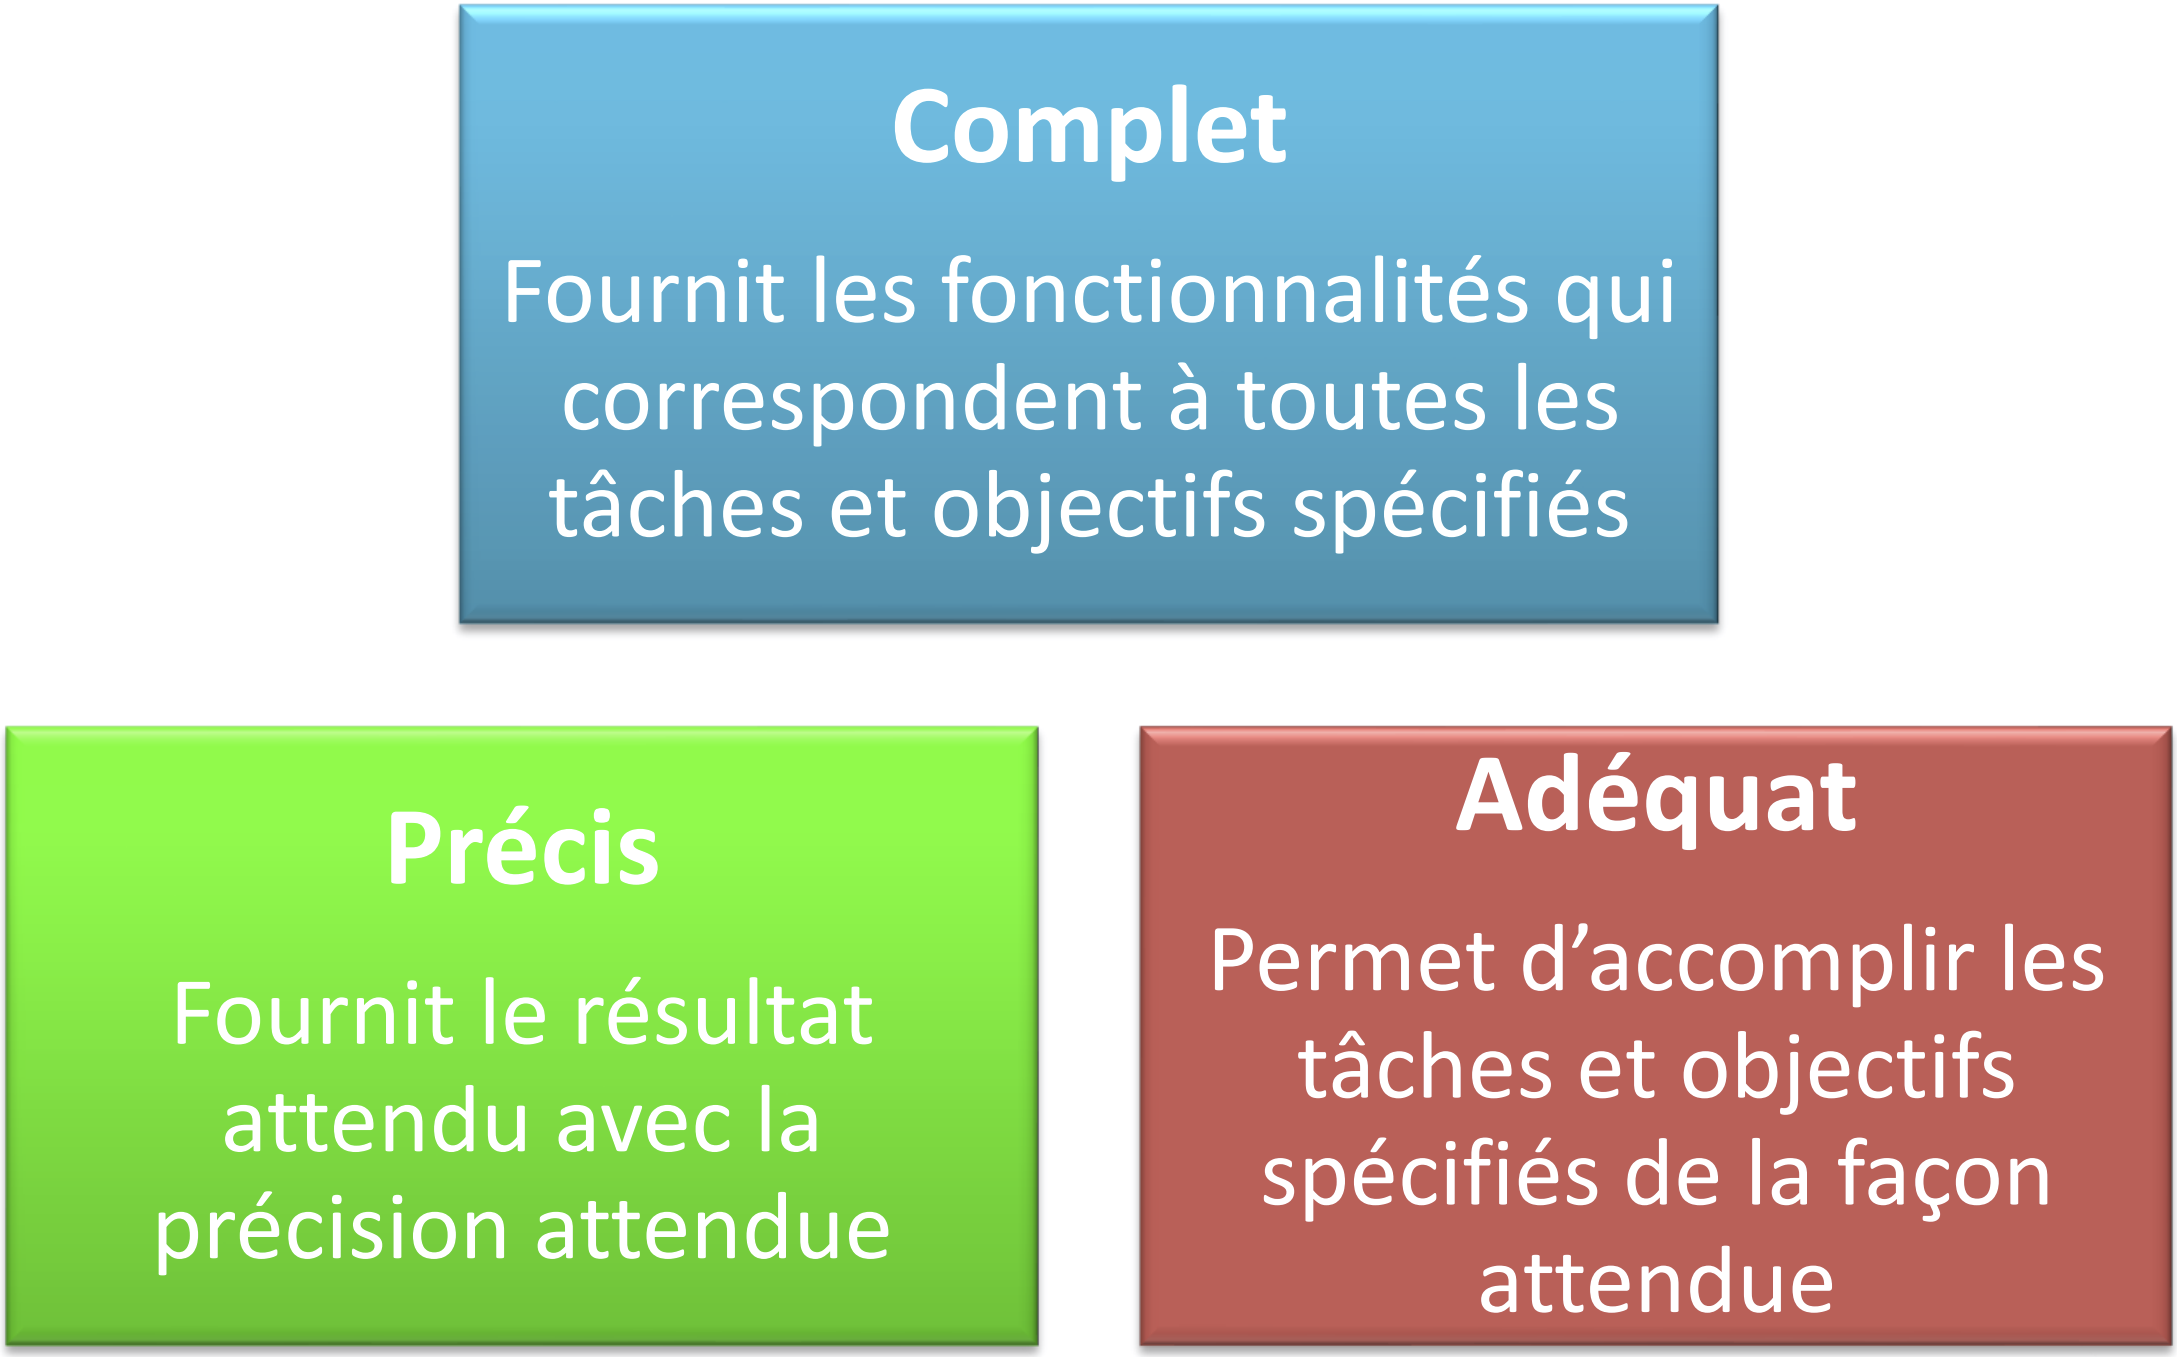
\includegraphics[width=0.35\textwidth]{perti.png}
            \end{center}
        \end{figure}


        \section{Performance}
        \begin{Concept}{Performance}{}
            Le logiciel présente des \textbf{performances relatives} aux ressources utilisée 
        \end{Concept}


         \begin{figure}[H]
            \begin{center}
                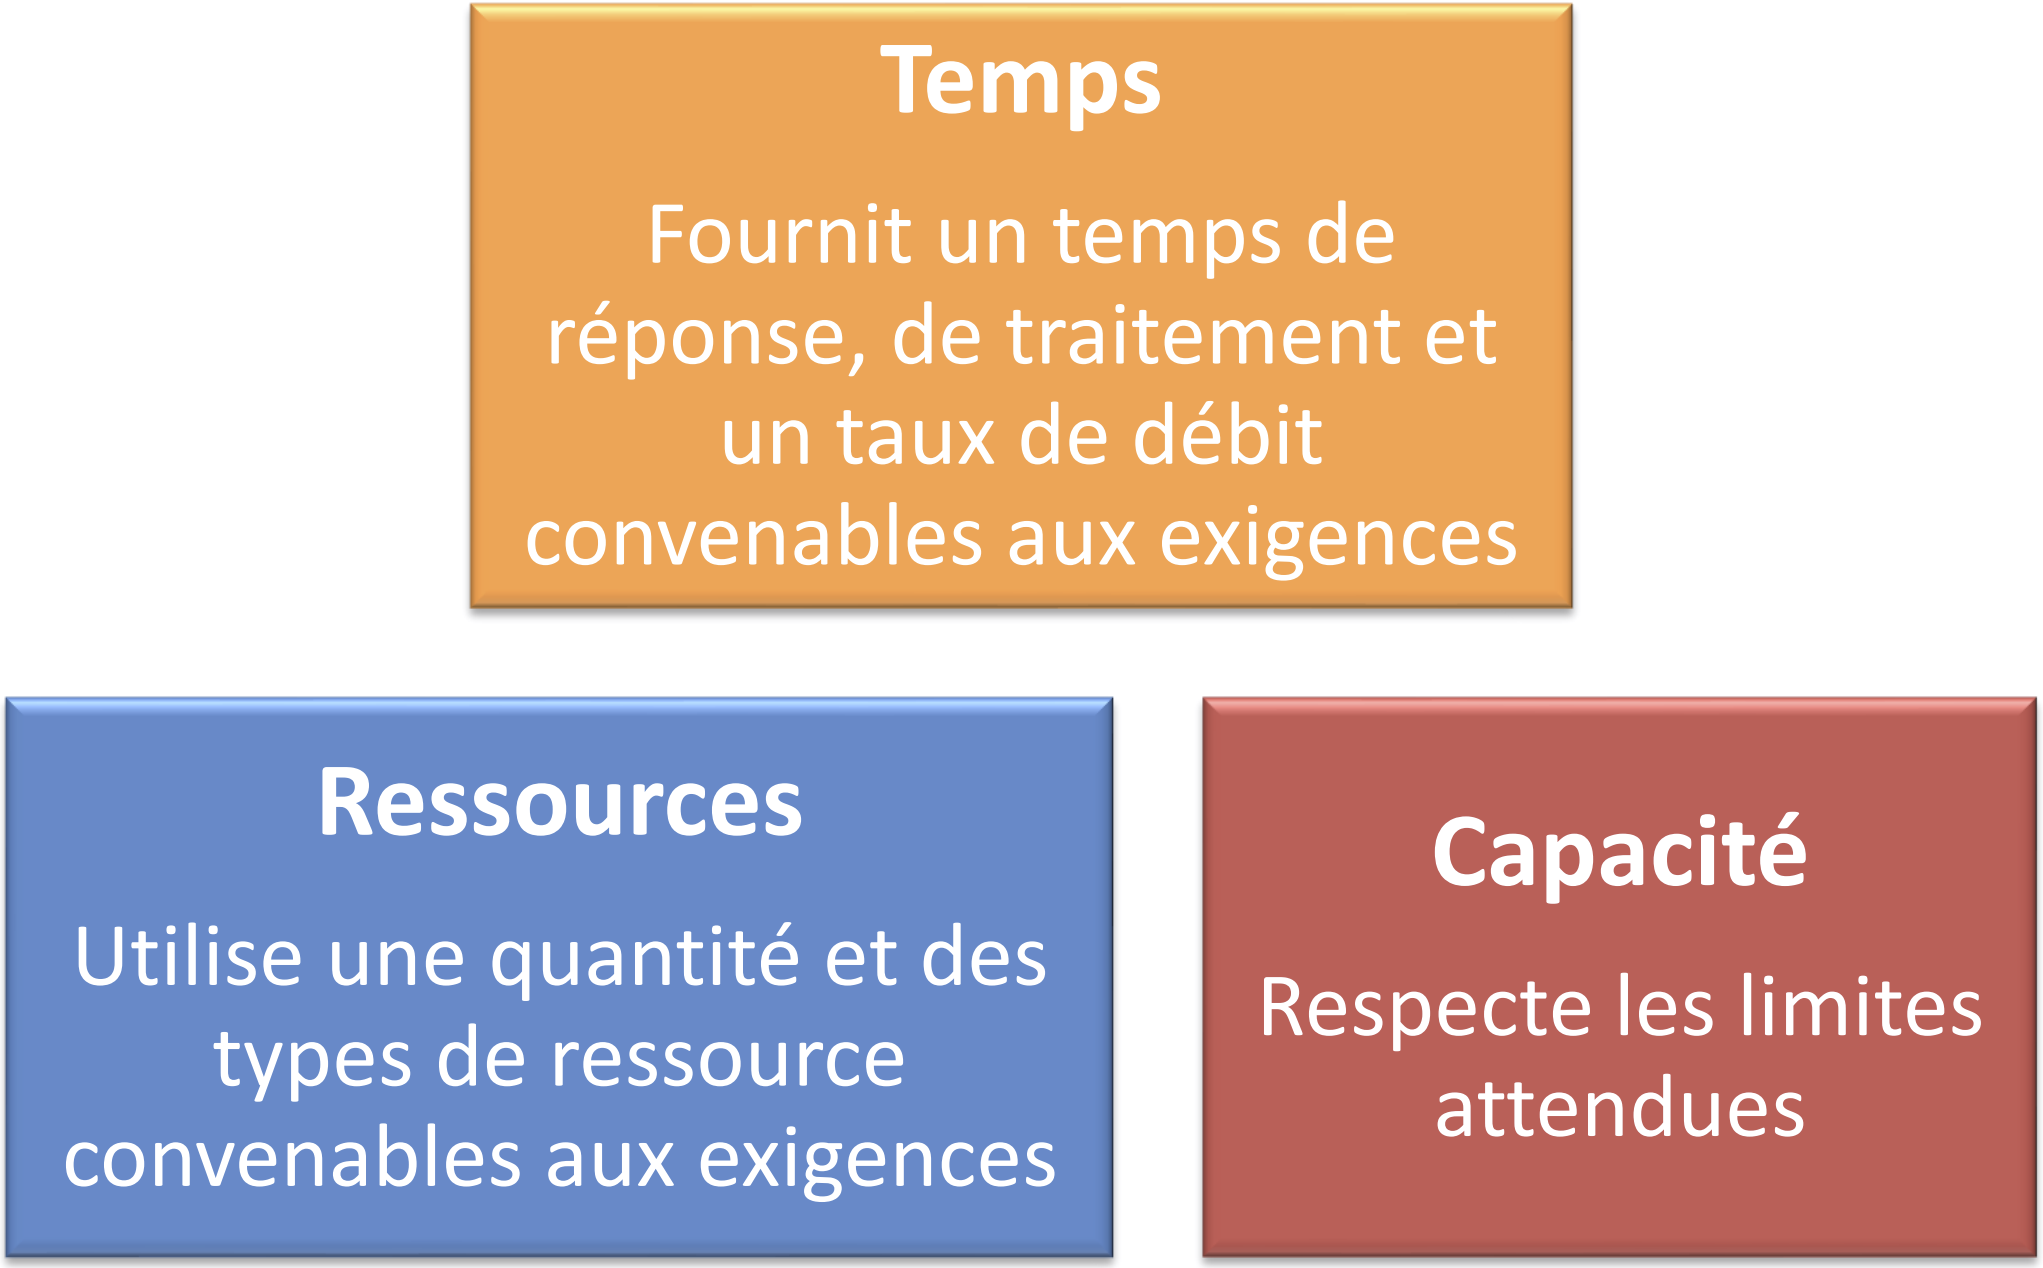
\includegraphics[width=0.35\textwidth]{perfo.png}
            \end{center}
        \end{figure}
       



        \section{Compatibilité}
        
        \begin{Concept}{Compatibilité}{}
            Deux modules peuvent échanger des informations et ou effectuer leurs tâches,
            tout en partageant le même environnement (matériel ou logiciel).
        \end{Concept}

        \begin{figure}[H]
            \begin{center}
                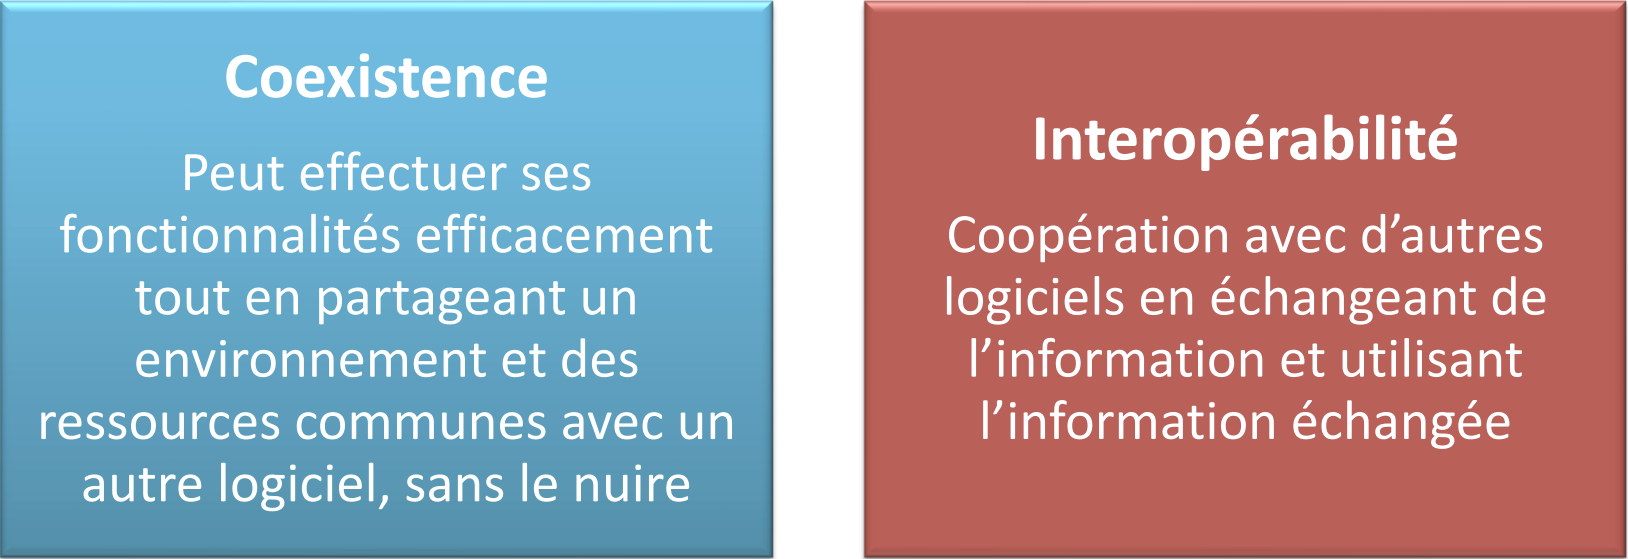
\includegraphics[width=0.35\textwidth]{cap3.png}
            \end{center}
        \end{figure}





        \section{Usabilité}
        
        \begin{Concept}{Usabilité}{}
            Logiciel peut être utilisé de manière efficace et efficiente par ces utilisateurs
            (humain), en procurant une expérience satisfaisante        
        \end{Concept}


        
        \begin{figure}[H]
            \begin{center}
                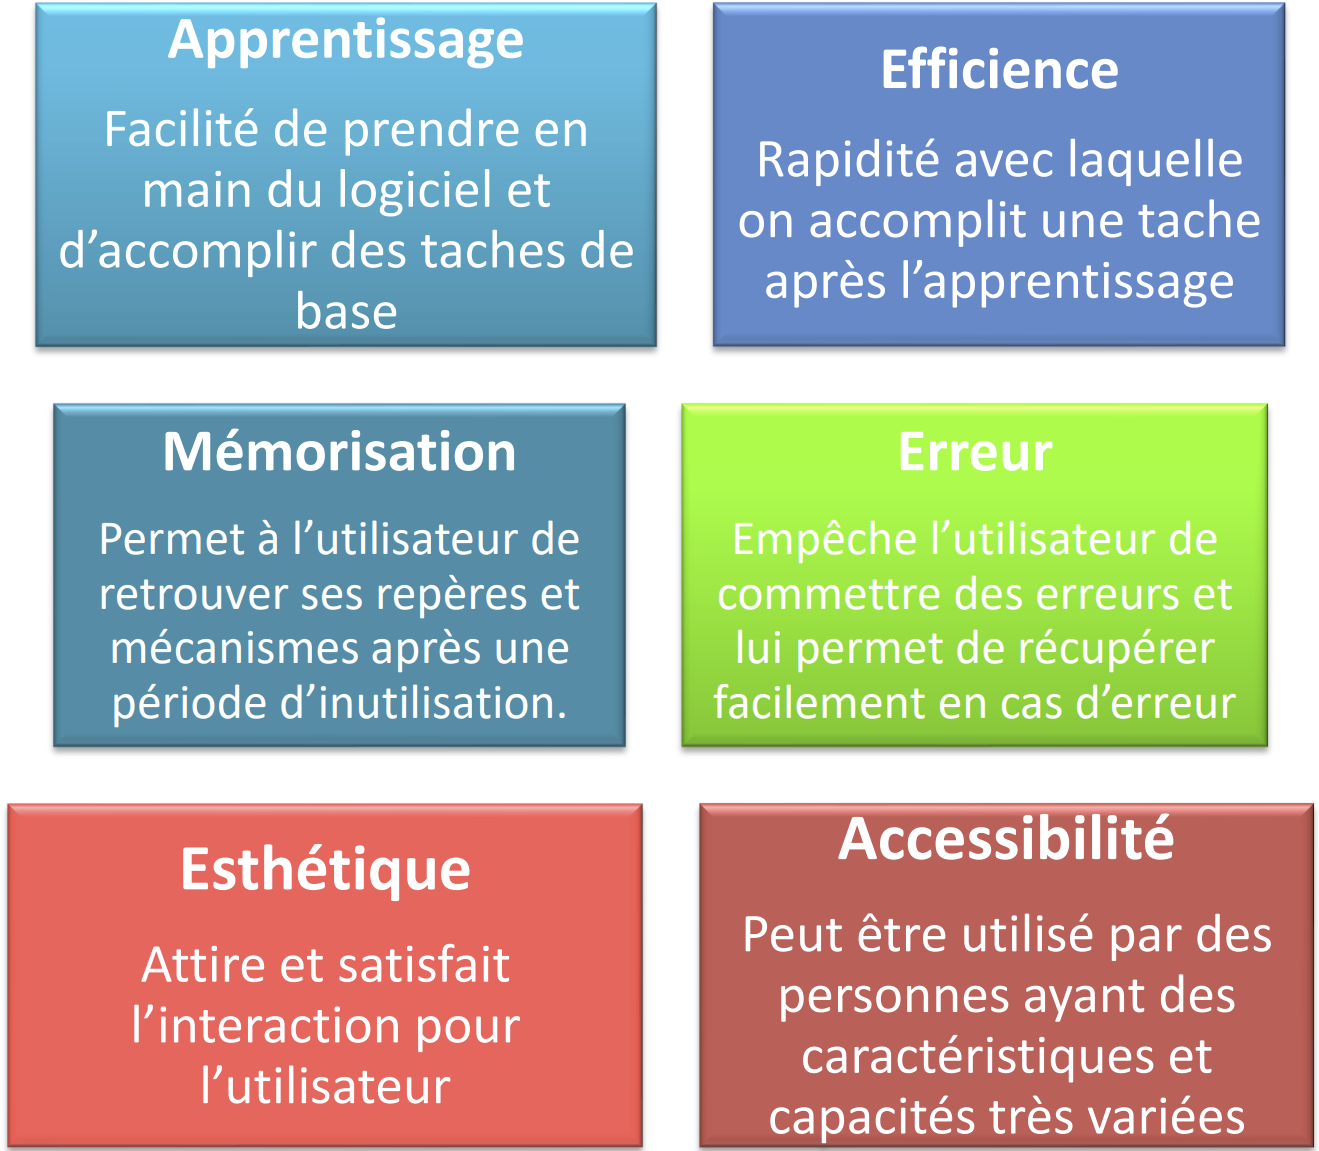
\includegraphics[width=0.35\textwidth]{cap4.png}
            \end{center}
        \end{figure}



        \section{Fiabilité}
        
        \begin{Concept}{Fiabilité}{}
            Logiciel performe des fonctionnalités attendues dans des conditions attendues
            sur une durée attendue.        
    \end{Concept}

        \begin{figure}[H]
            \begin{center}
                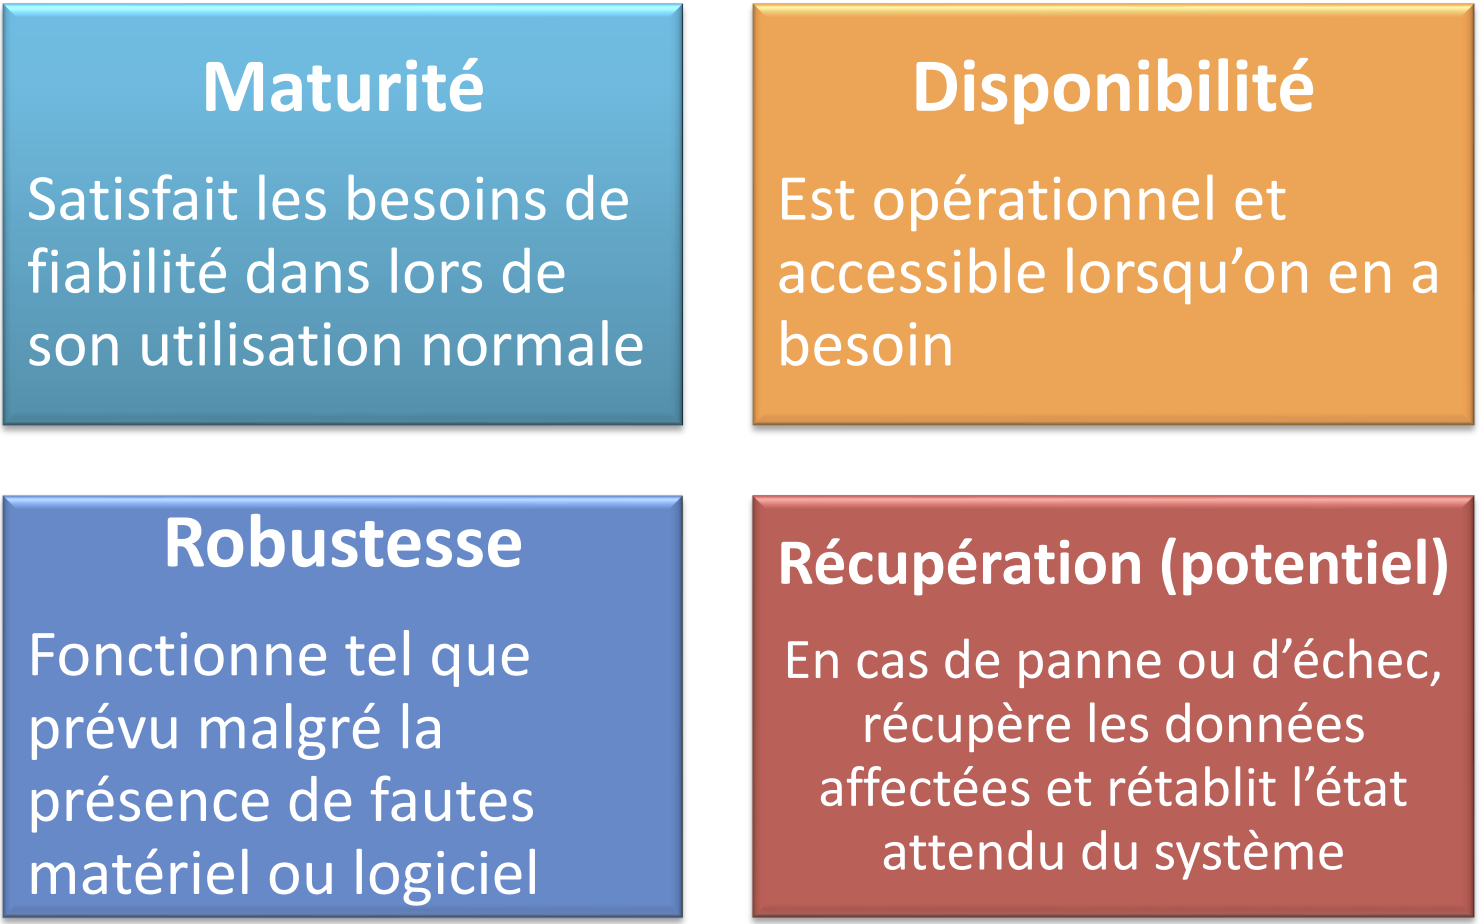
\includegraphics[width=0.35\textwidth]{cap5.png}
            \end{center}
        \end{figure}


        \section{Sécurité}
        
        \begin{Concept}{Sécurité}{}
           Logiciel protège l’information pour que les utilisateurs aient les accès requis
            conformément à leur type/rôle et niveau d’autorisation.
        \end{Concept}
        
    
        \begin{figure}[H]
            \begin{center}
                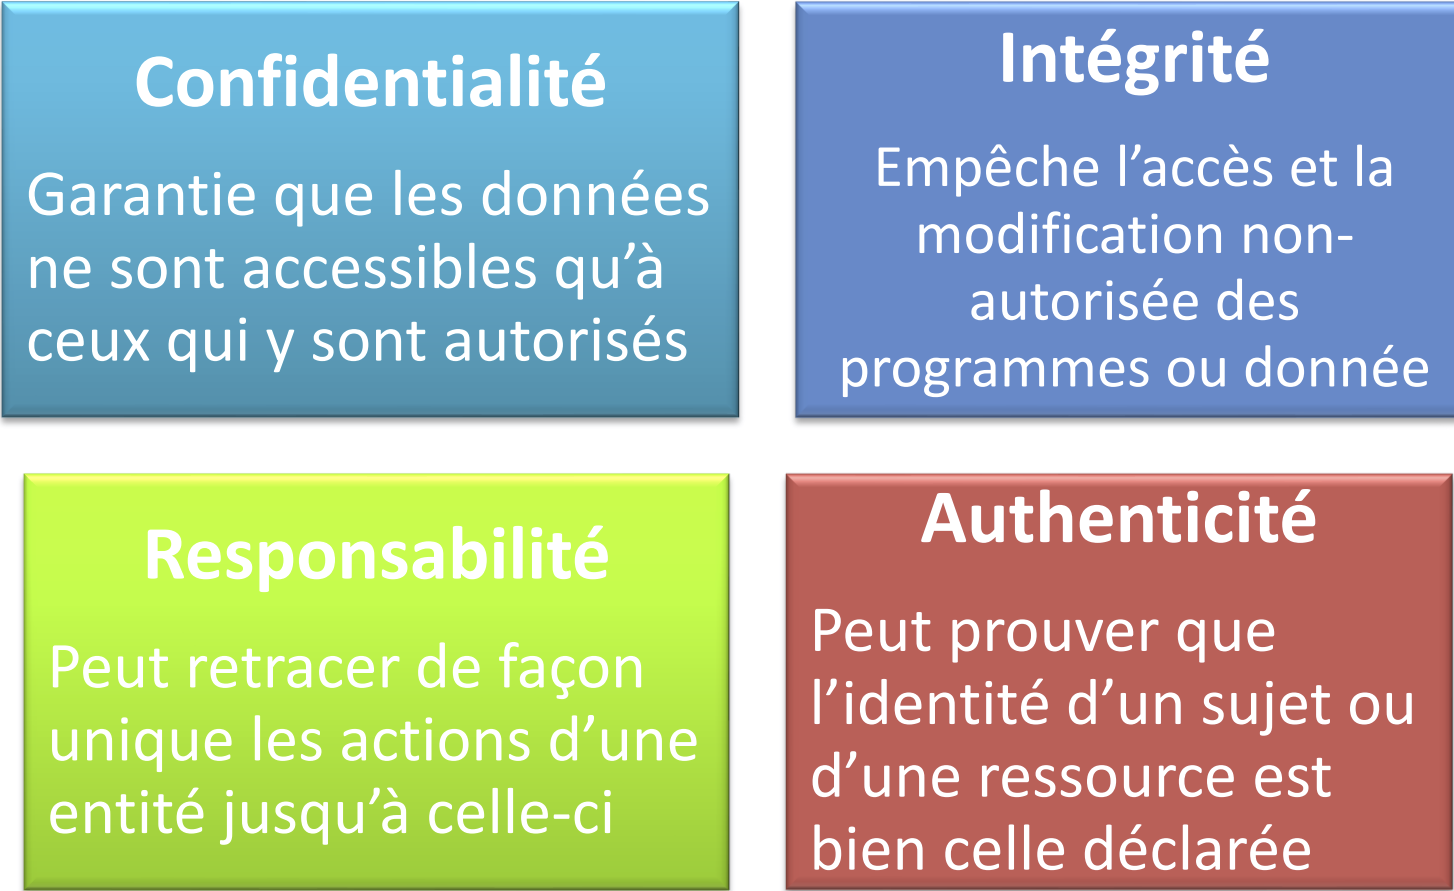
\includegraphics[width=0.35\textwidth]{cap6.png}
            \end{center}
        \end{figure}



        \section{Maintenabilité}
        
        \begin{Concept}{Maintenabilité}{}
            Logiciel peut être modifié efficacement pour l’adapter aux changements dans
            l’environnement et dans les exigences.
        \end{Concept}


        


        \begin{figure}[H]
            \begin{center}
                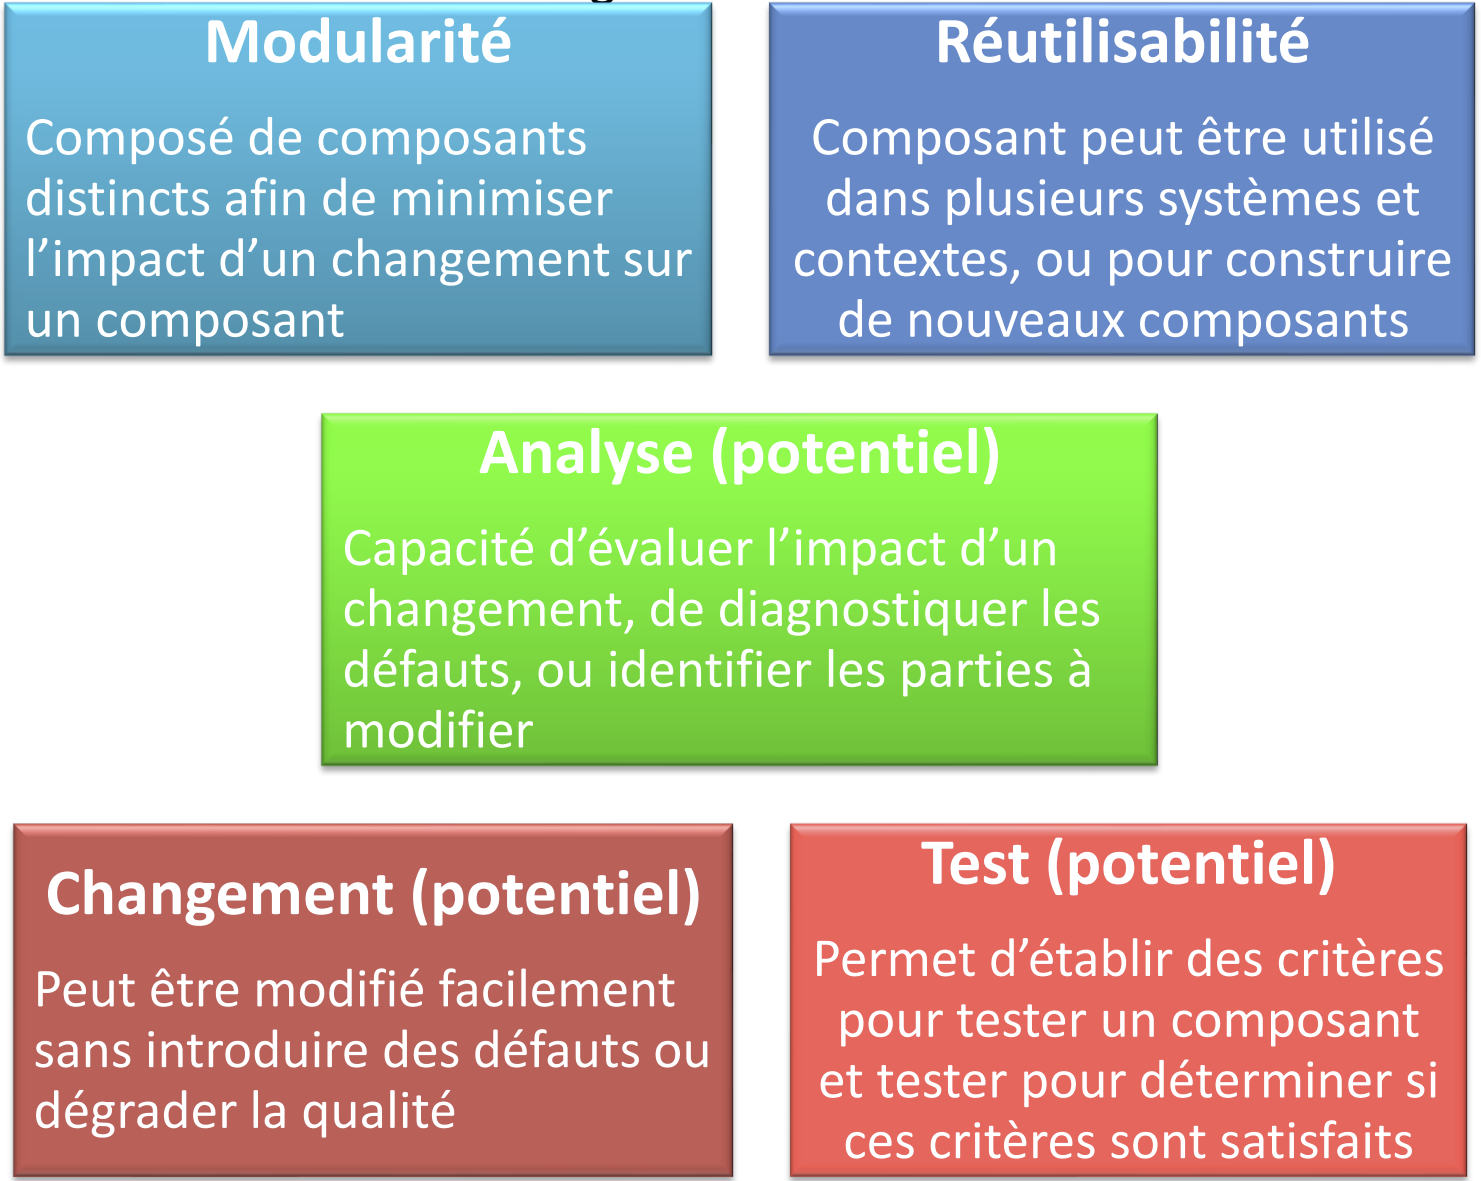
\includegraphics[width=0.35\textwidth]{cap7.png}
            \end{center}
        \end{figure}


        \section{Transférabilité}
        
        \begin{Concept}{Transférabilité}{}
            Logiciel peut être transféré d’un environnement (logiciel ou matériel) à un autre
        \end{Concept}



        \begin{figure}[H]
            \begin{center}
                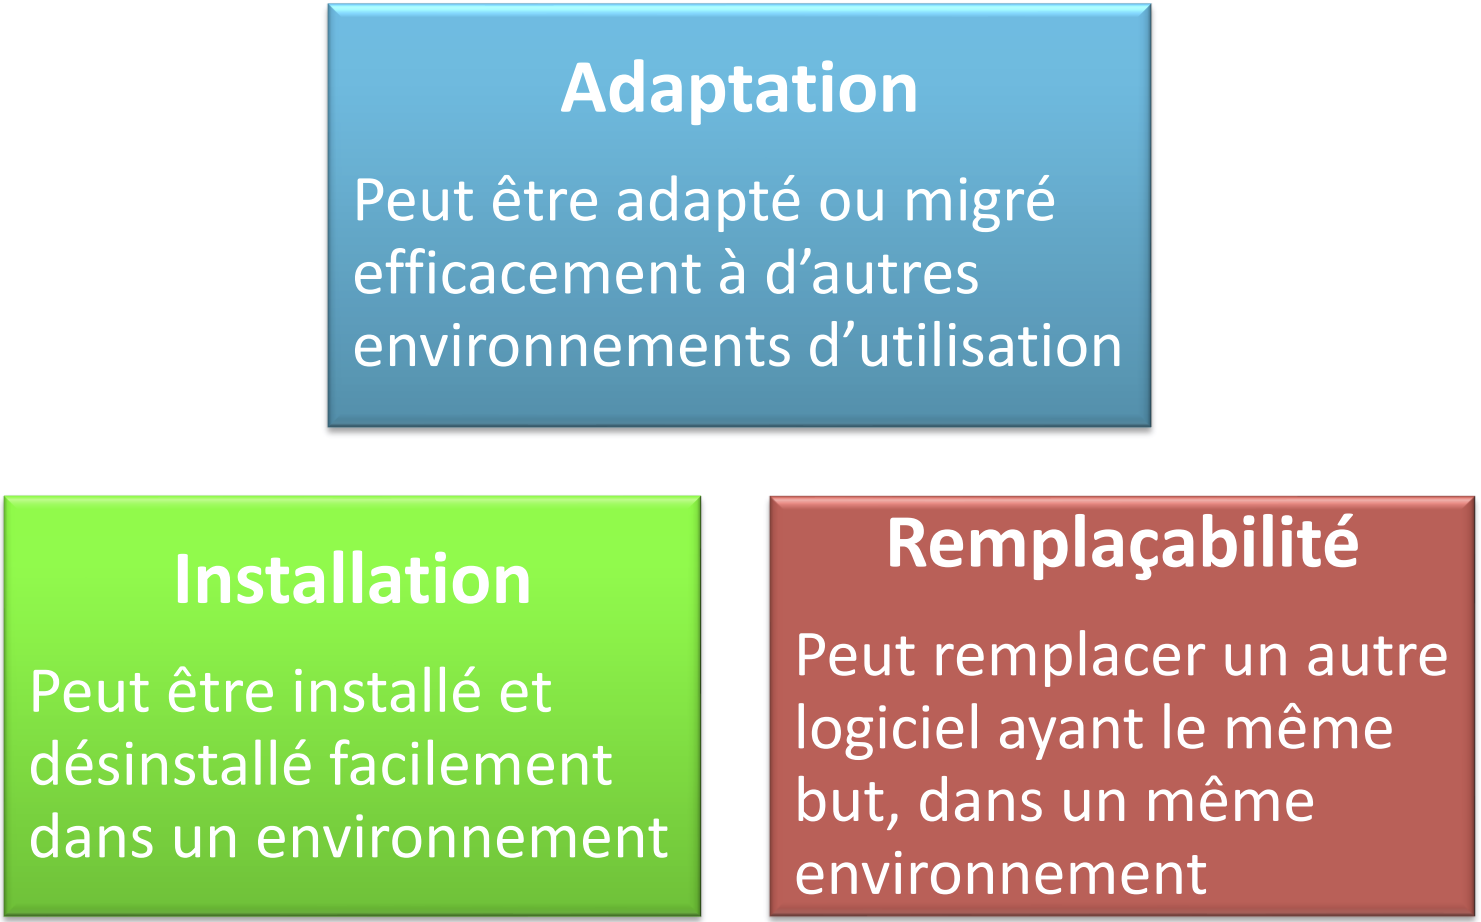
\includegraphics[width=0.35\textwidth]{cap8.png}
            \end{center}
        \end{figure}

        \section{Assurance Qualité}


        \begin{Concept}{Assurance Qualité}{}
           \textbf{Role} : s'assurer que l'équipe de développement a fournit un \textcolor{myb}{travail de qualité}   
           \begin{itemize}
            \item À la fin de chaque Workflow 
            \item Quand le produti est complété 
            \item AQ doit être appliquée au processus de développement. 
            Il n'y a pas de \textbf{hiérarchie} entre l'équipe \texttt{AQ} et l'équipe de \texttt{Dev}      
           \end{itemize}
        \end{Concept}


        \begin{figure}[H]
            \begin{center}
                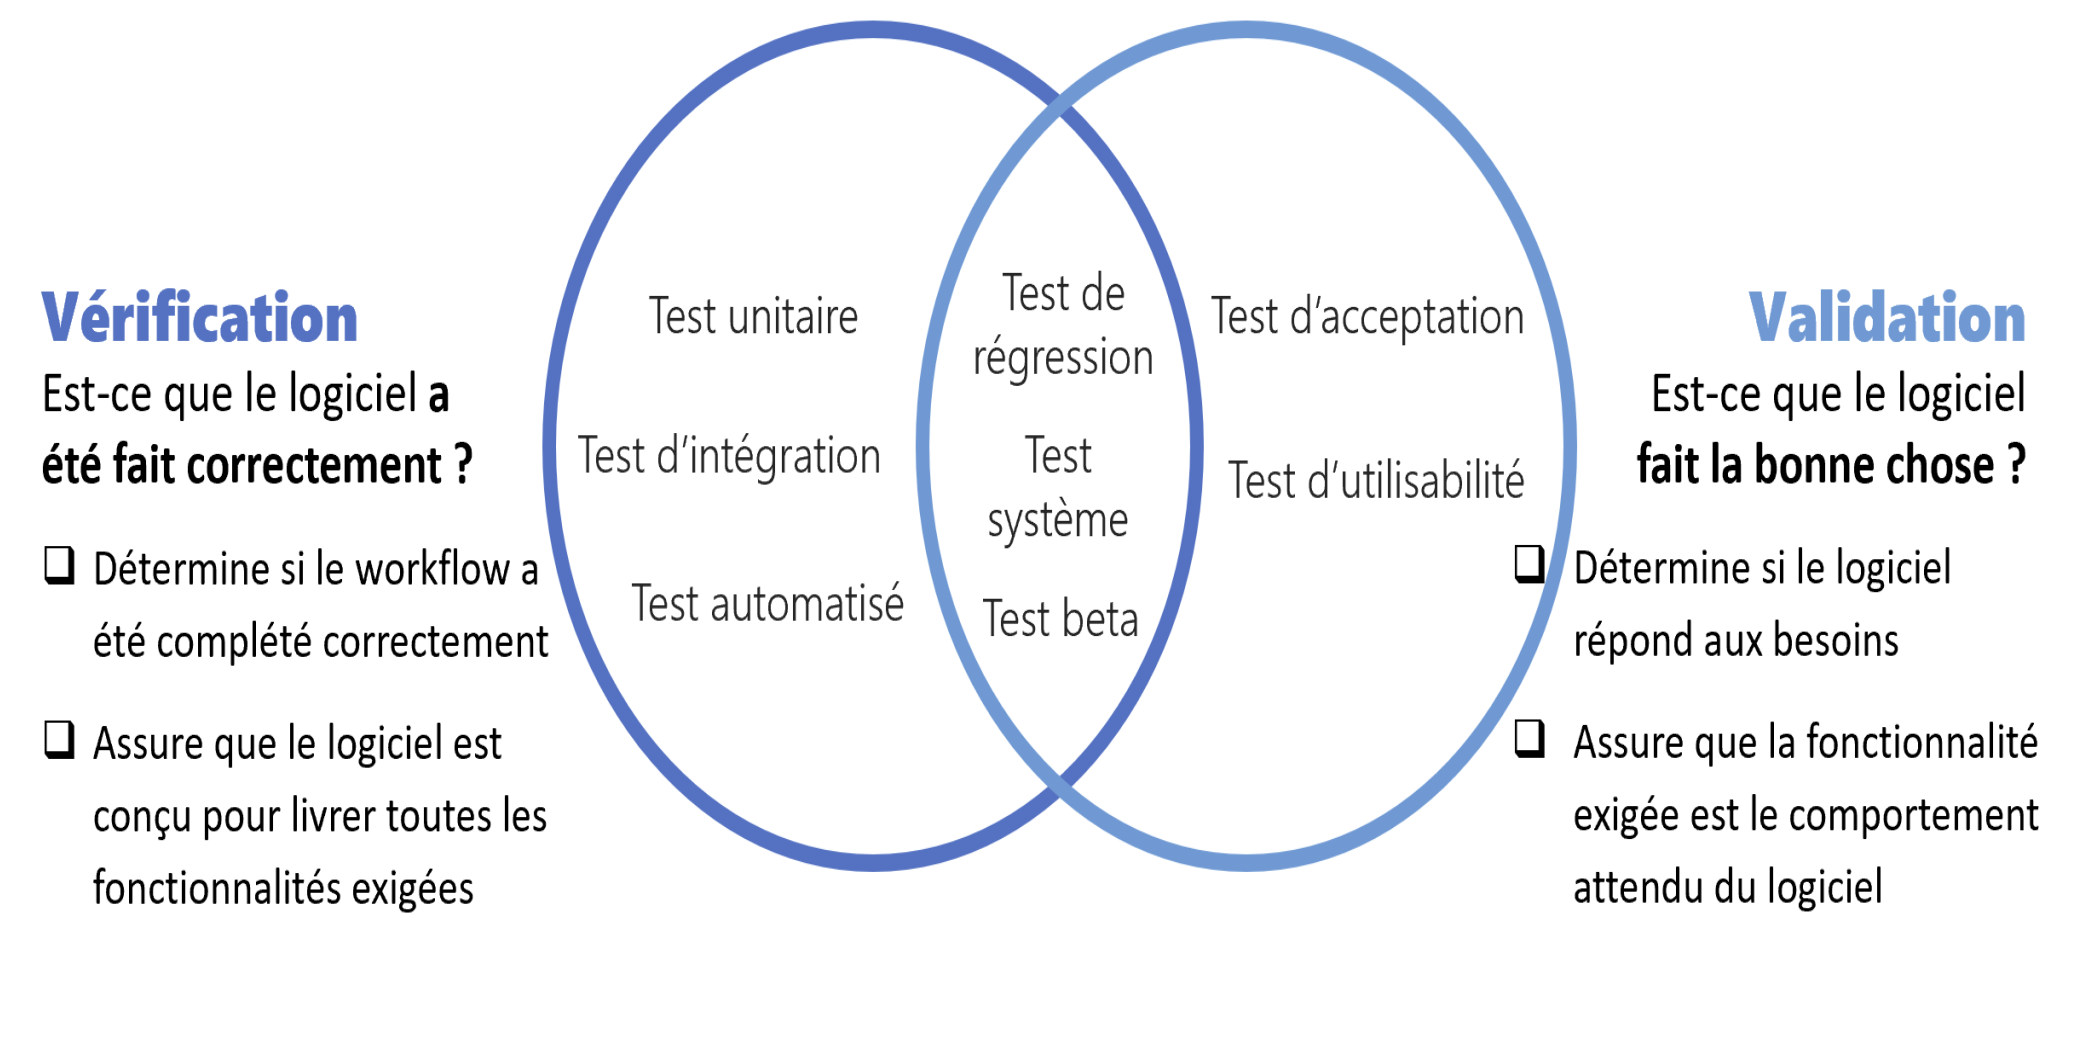
\includegraphics[width=0.40\textwidth]{VerifValid.png}
            \end{center}
        \end{figure}


        \section{Logiciel fiable}


        \begin{figure}[H]
        \begin{center}
            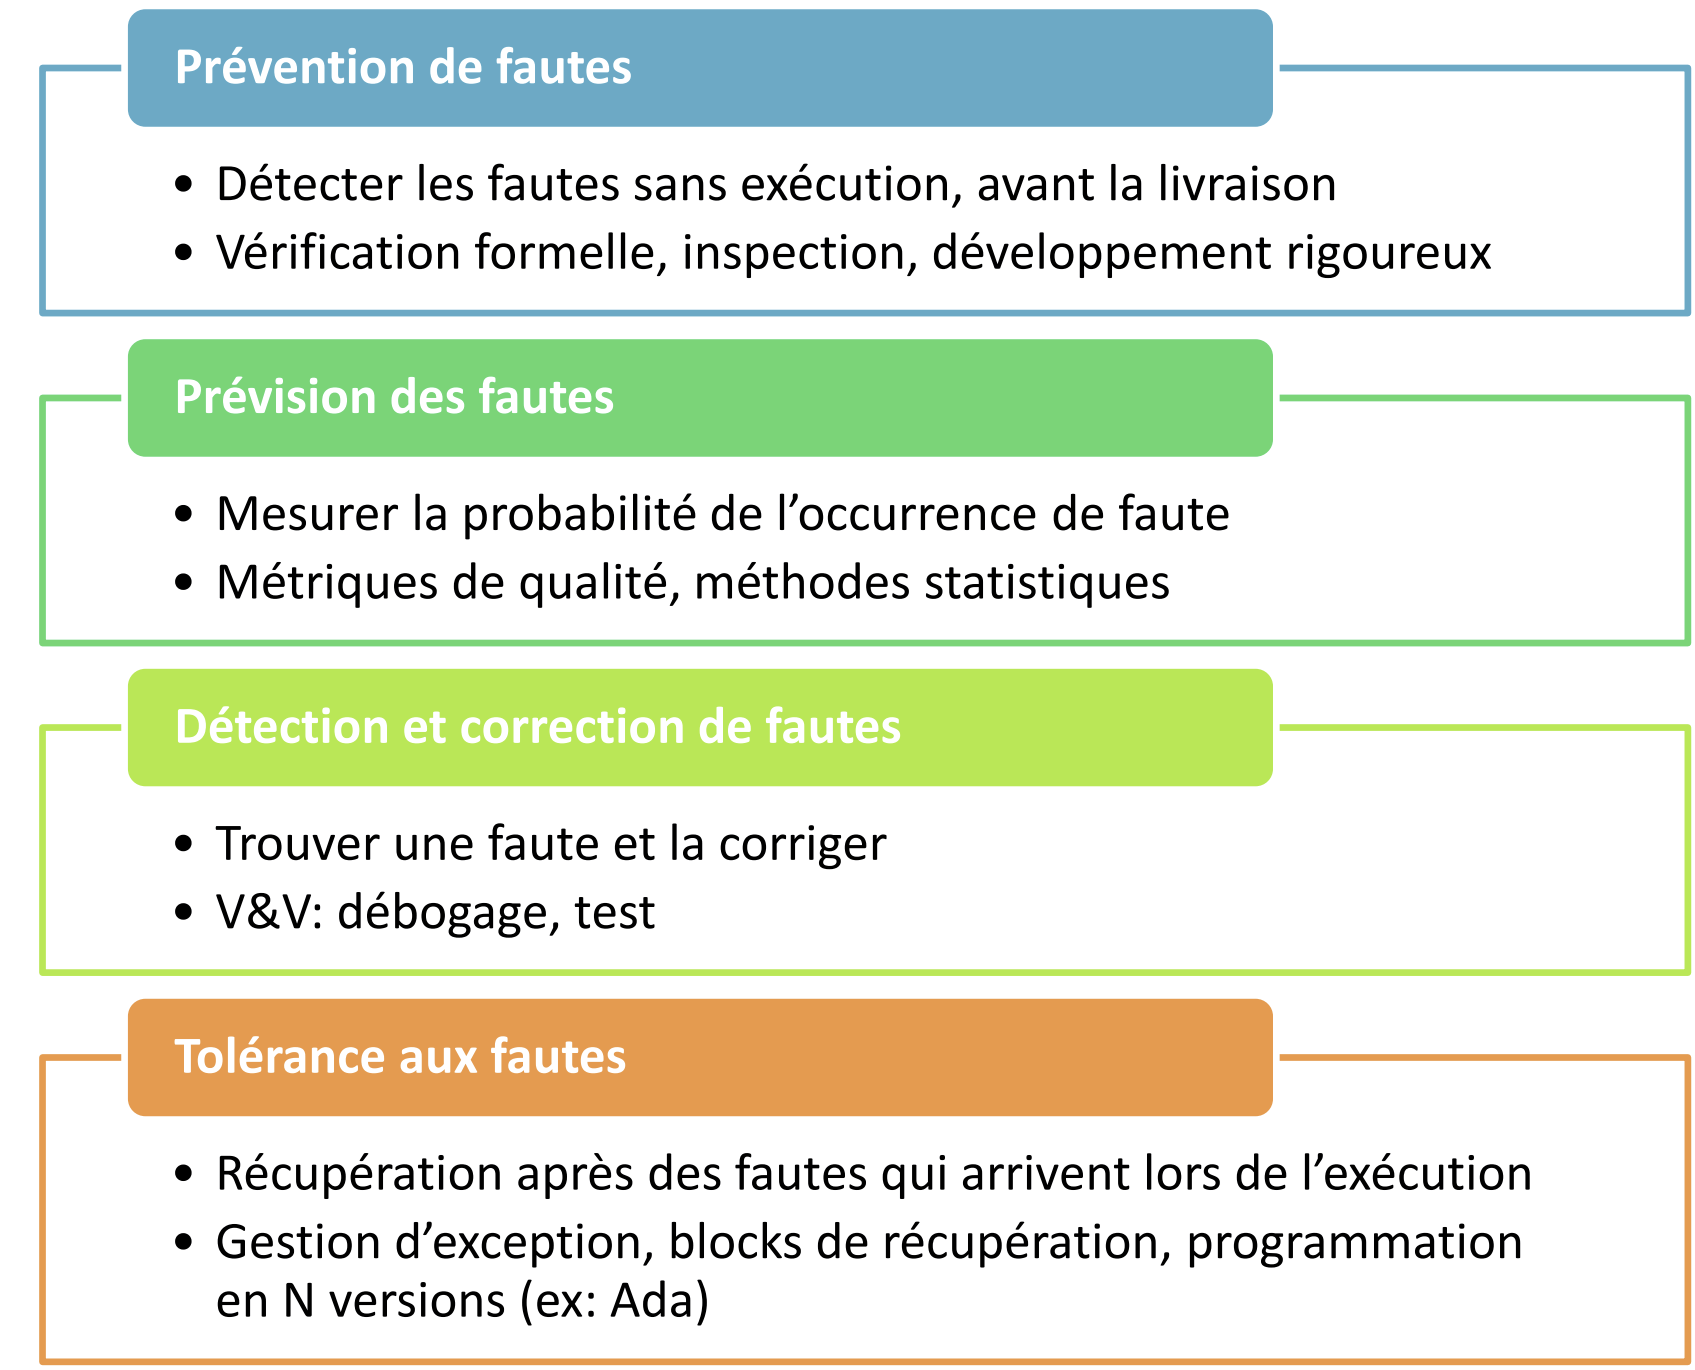
\includegraphics[width=0.45\textwidth]{LogiFiable}
        \end{center}
       \end{figure}

       \section{Vérifinication sans exécution}


       \begin{Concept}{Vérification sans exécution}{}
           Processus par lequel on teste le logiciel en l'examinant visuellement. On vérifie tous les 
           artéfacts produits à chaque workflow; on évite d'examiner \textcolor{myb}{son propre travail}  
       \end{Concept}


       \begin{figure}[H]
        \begin{center}
            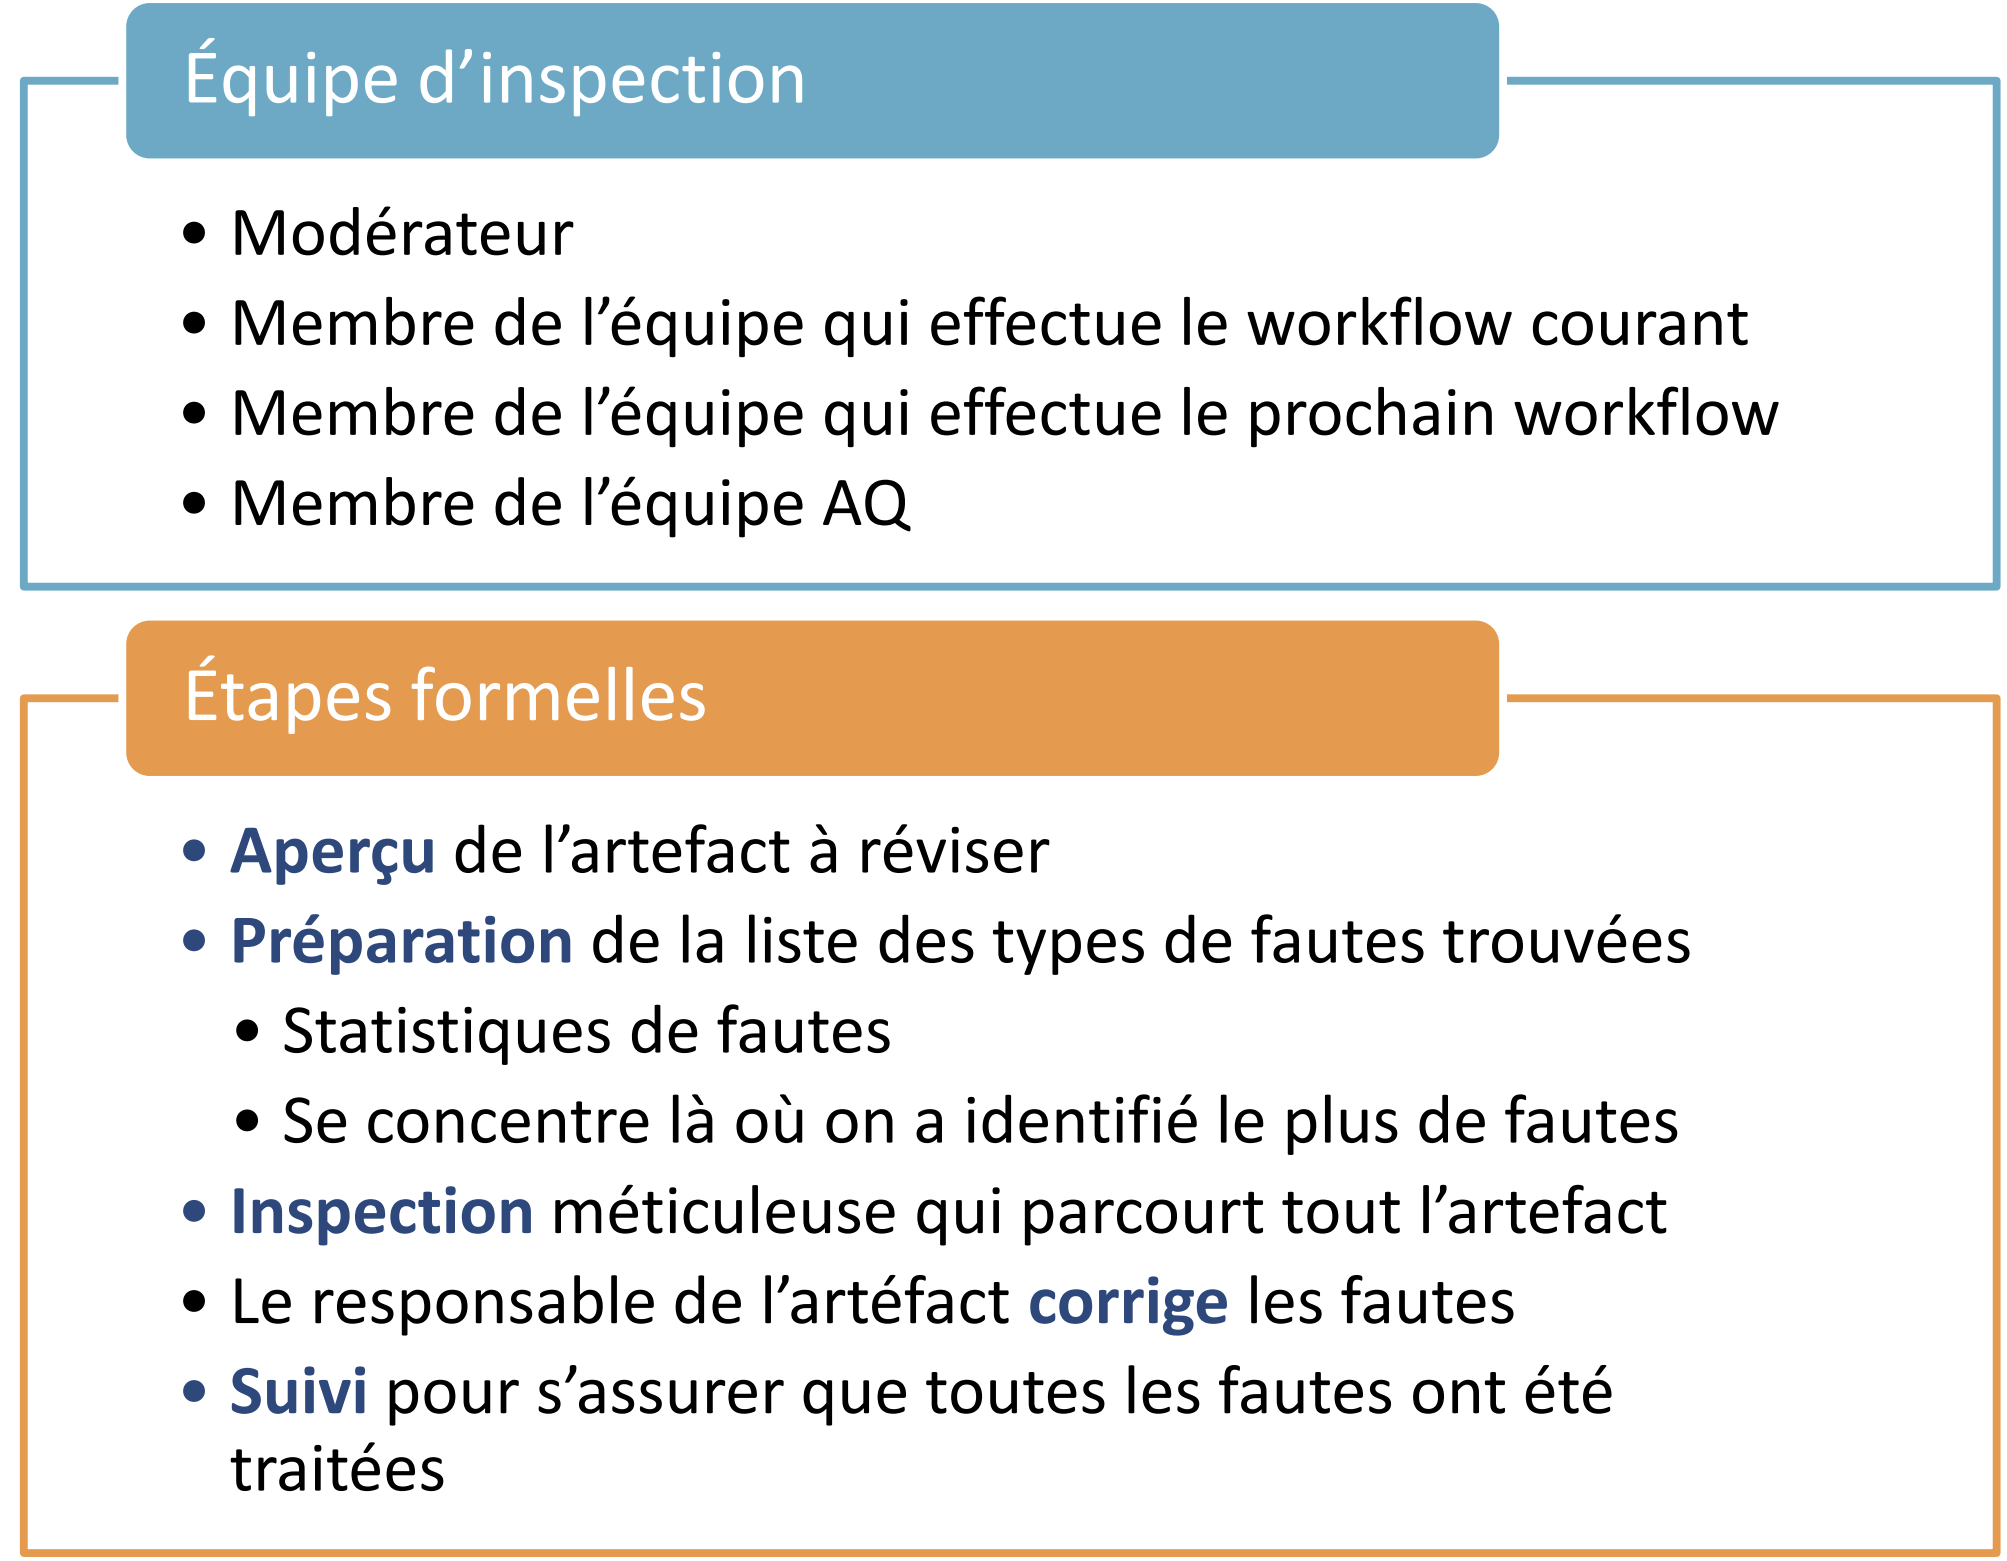
\includegraphics[width=0.45\textwidth]{inspection}
        \end{center}
       \end{figure}

       \begin{itemize}
        \item \textbf{Statistiques d'inspection}  
            \begin{itemize}
                \item[$\blacktriangleright$] Pour chaque workflow, on compare le taux d’erreur avec l’incrément 
                    précédent 
                \item[$\blacktriangleright$] Réagir s’il y a un nombre disproportionné de fautes dans un artéfact
                \item[$\rhd$] Reconcevoir dès le début devient une bonne alternative
            \end{itemize}
        \item \textbf{Métriques d’inspection}  
            \begin{itemize}
                \item[$\blacktriangleright$] Densité de fautes (fautes par KLOC*inspectées)
                \item[$\blacktriangleright$] Taux d’inspection (diagramme/page révisé par heure)
                \item[$\blacktriangleright$] Taux de détection de fautes (fautes détectées par heure)
                \item[$\blacktriangleright$] Efficacité de détection de fautes (nombre de fautes majeures
                        détectées par heure)
            \end{itemize}
       \end{itemize}

       \section{Code Review}


       \begin{figure}[H]
        \begin{center}
            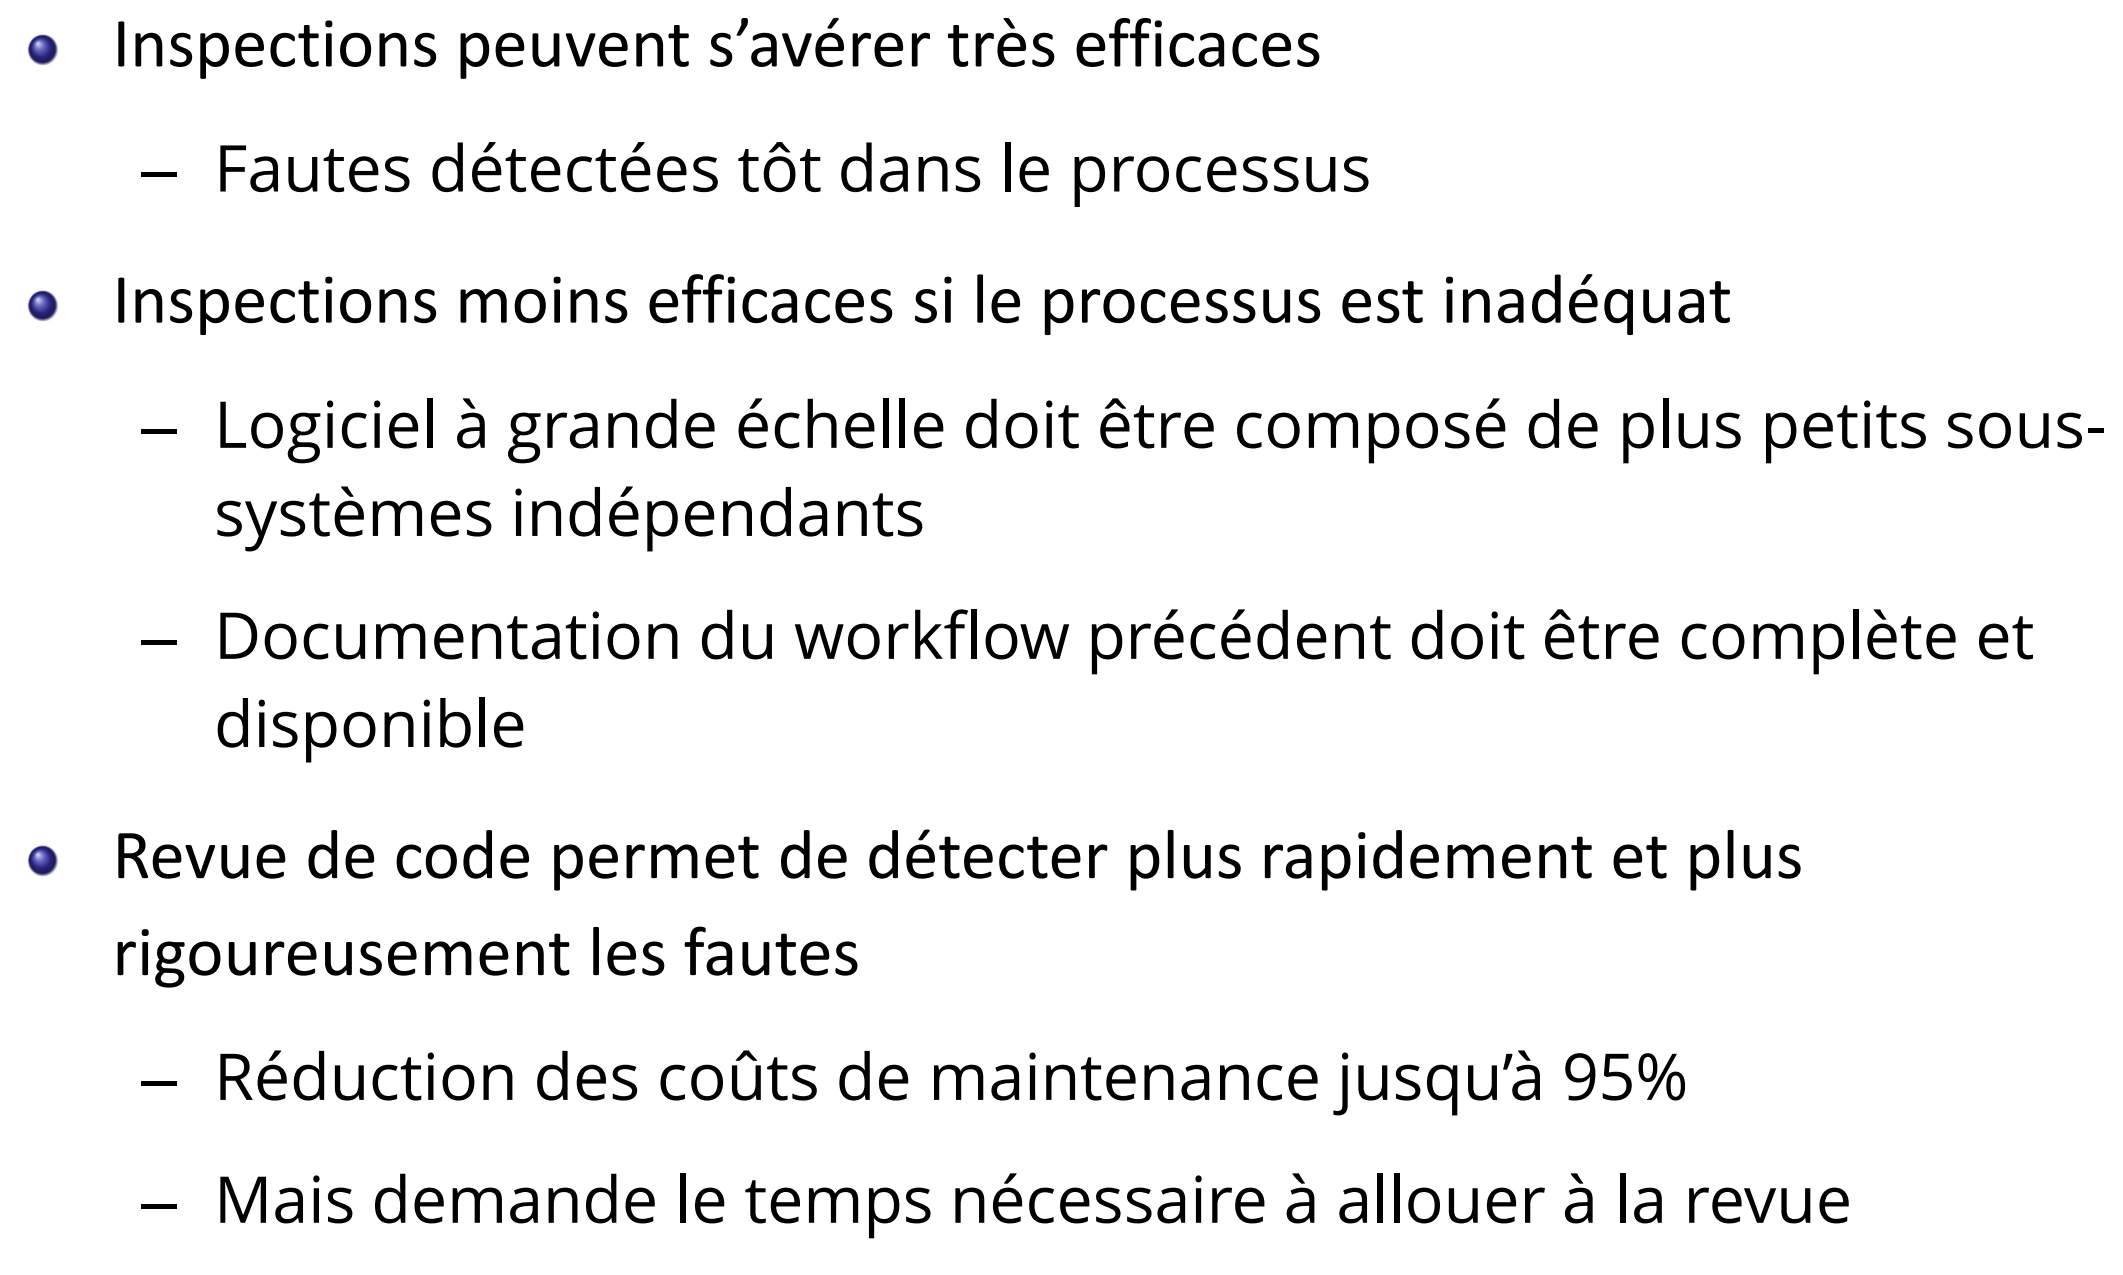
\includegraphics[width=0.38\textwidth]{CodeReview}
        \end{center}
       \end{figure}


       \section{Test}


       \begin{note}{}{}
           Tester un logiciel, c’est l’exécuter dans le but 
           de le faire \textbf{échouer}
       \end{note}


       \begin{Definitionx}{Test}{}
           Processus par lequel on tente d'identifier les différences entre 
           le comportement \textbf{attendu} et le comportement \textbf{observé}. C'est une 
           \textit{technique de détection de fautes} qui tente de \textbf{faire échouer}     
           le logiciel ou l'amener à un état erroné, de façon planifiée. 
       \end{Definitionx}

       \begin{itemize}
        \item \textbf{Vérification basée sur l'exécution}  
       \end{itemize}

       \begin{figure}[H]
        \begin{center}
            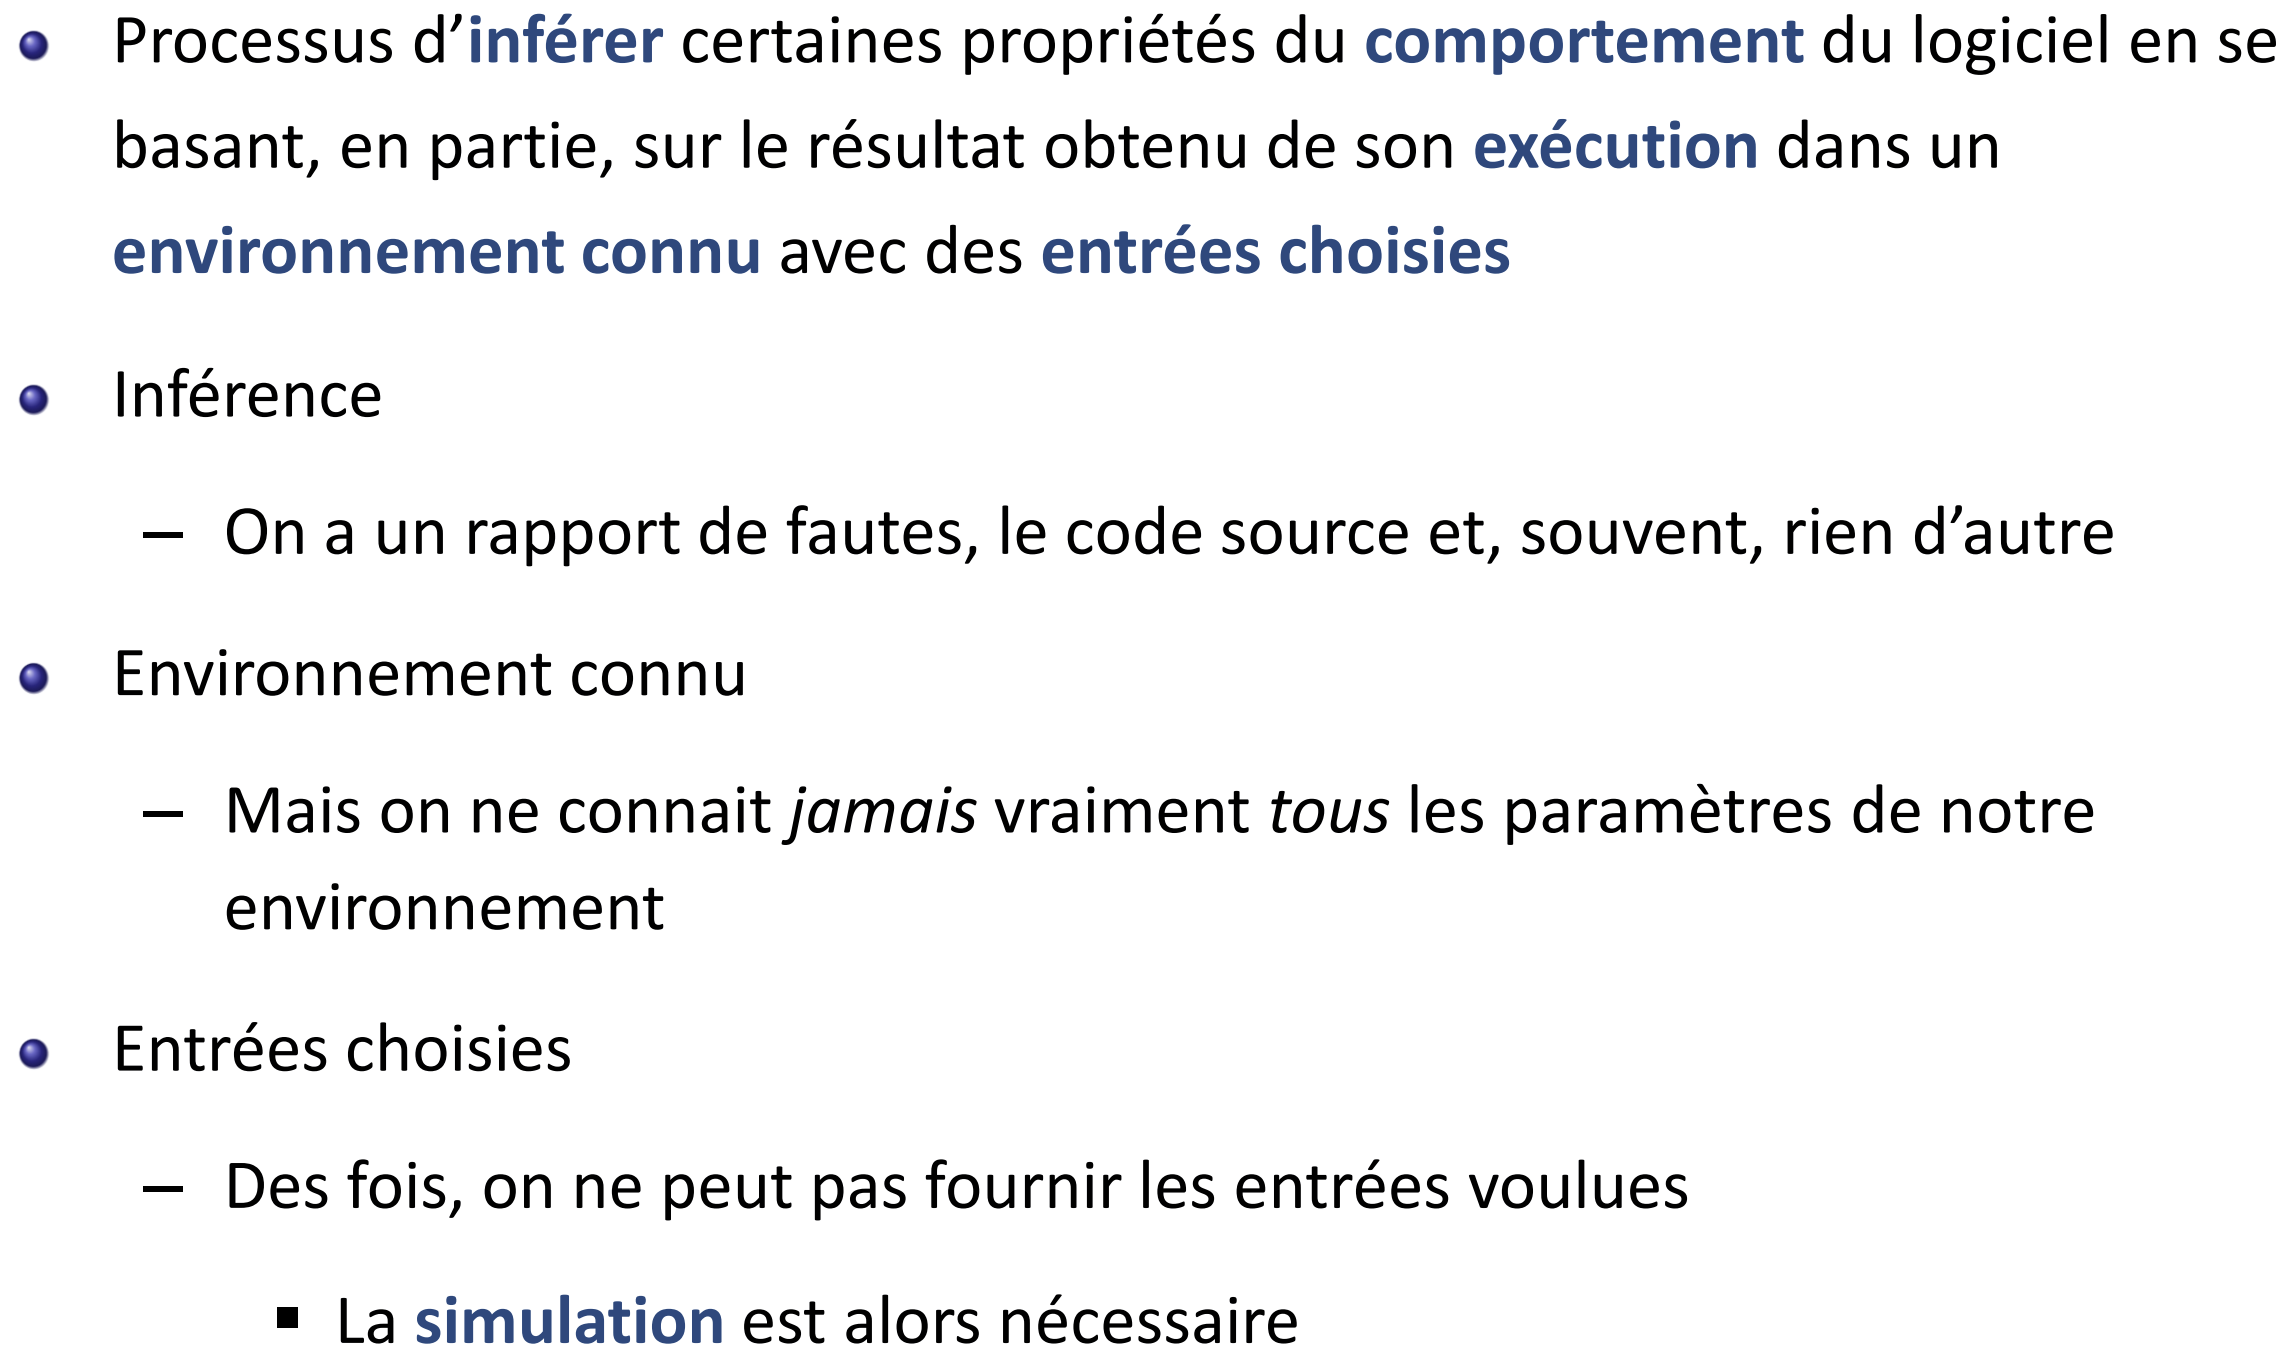
\includegraphics[width=0.38\textwidth]{Verif.png}
        \end{center}
       \end{figure}

       \begin{itemize}
        \item \textbf{\textcolor{red}{Attention}  }  
            \begin{itemize}
                \item[$\blacktriangleright$] Les tests supposent que la spécification est correcte
                \item[$\rhd$] Il faut toujours \textbf{valider les spécifications} avant de tester.   
            \end{itemize}
       \end{itemize}


       \begin{note}{}{}
           La \textbf{démonstration d’exactitude} est une technique de vérification sous-utilisée 
           en génie logiciel. Les ingénieurs logiciel n’ont pas assez de connaissances mathématiques 
           pour rédiger les démonstrations. Bien que, la plupart des informaticiens ont la capacité de l’apprendre, 
           Démontrer coûte trop cher pour être pratique. Et la \textcolor{myb}{viabilité économique}
           est déterminé par une analyse coût-avantage 
       \end{note}

       \section{Stratégies pour tester}


       \begin{figure}[H]
        \begin{center}
            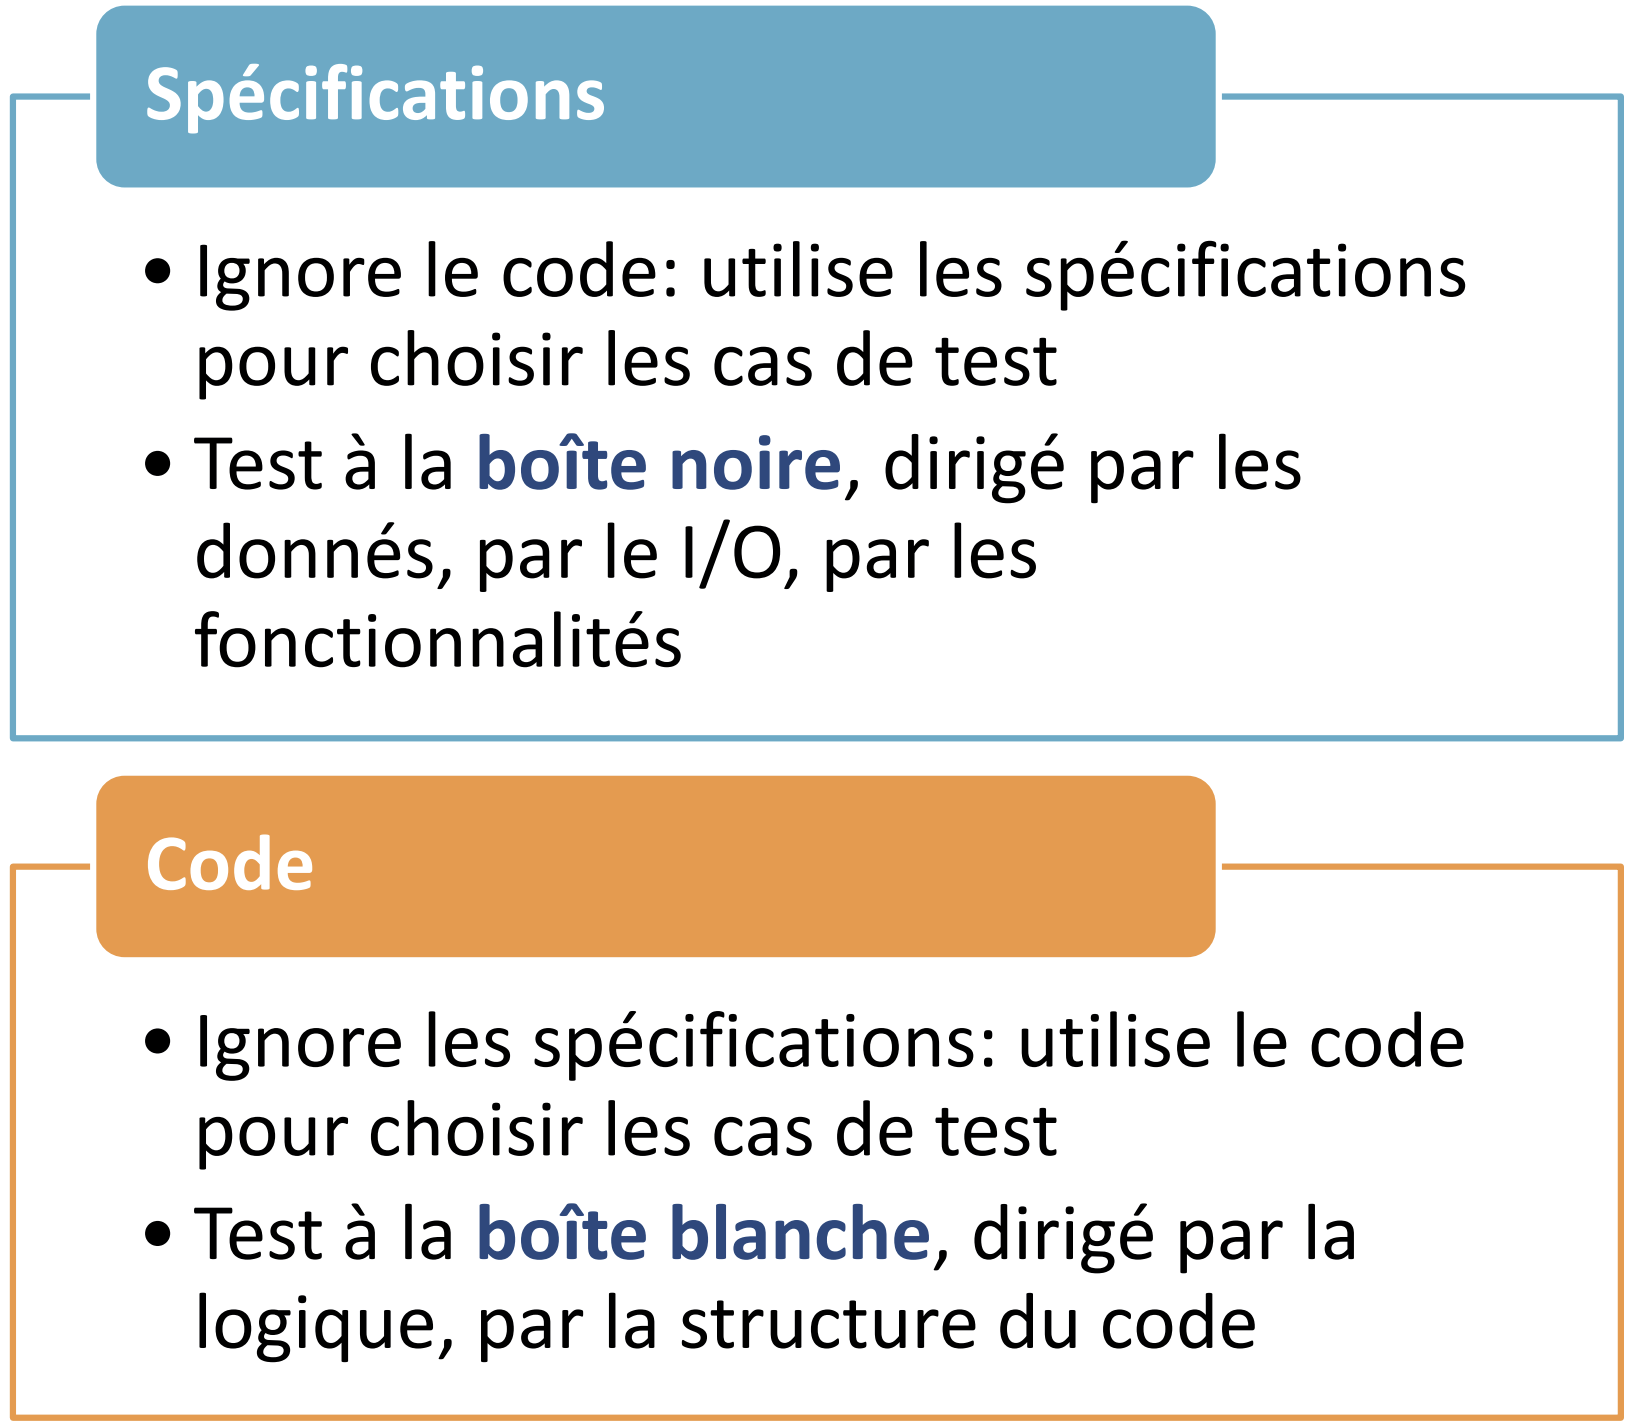
\includegraphics[width=0.45\textwidth]{strattest1.png}
        \end{center}
       \end{figure}
       
       


       \begin{figure}[H]
        \begin{center}
            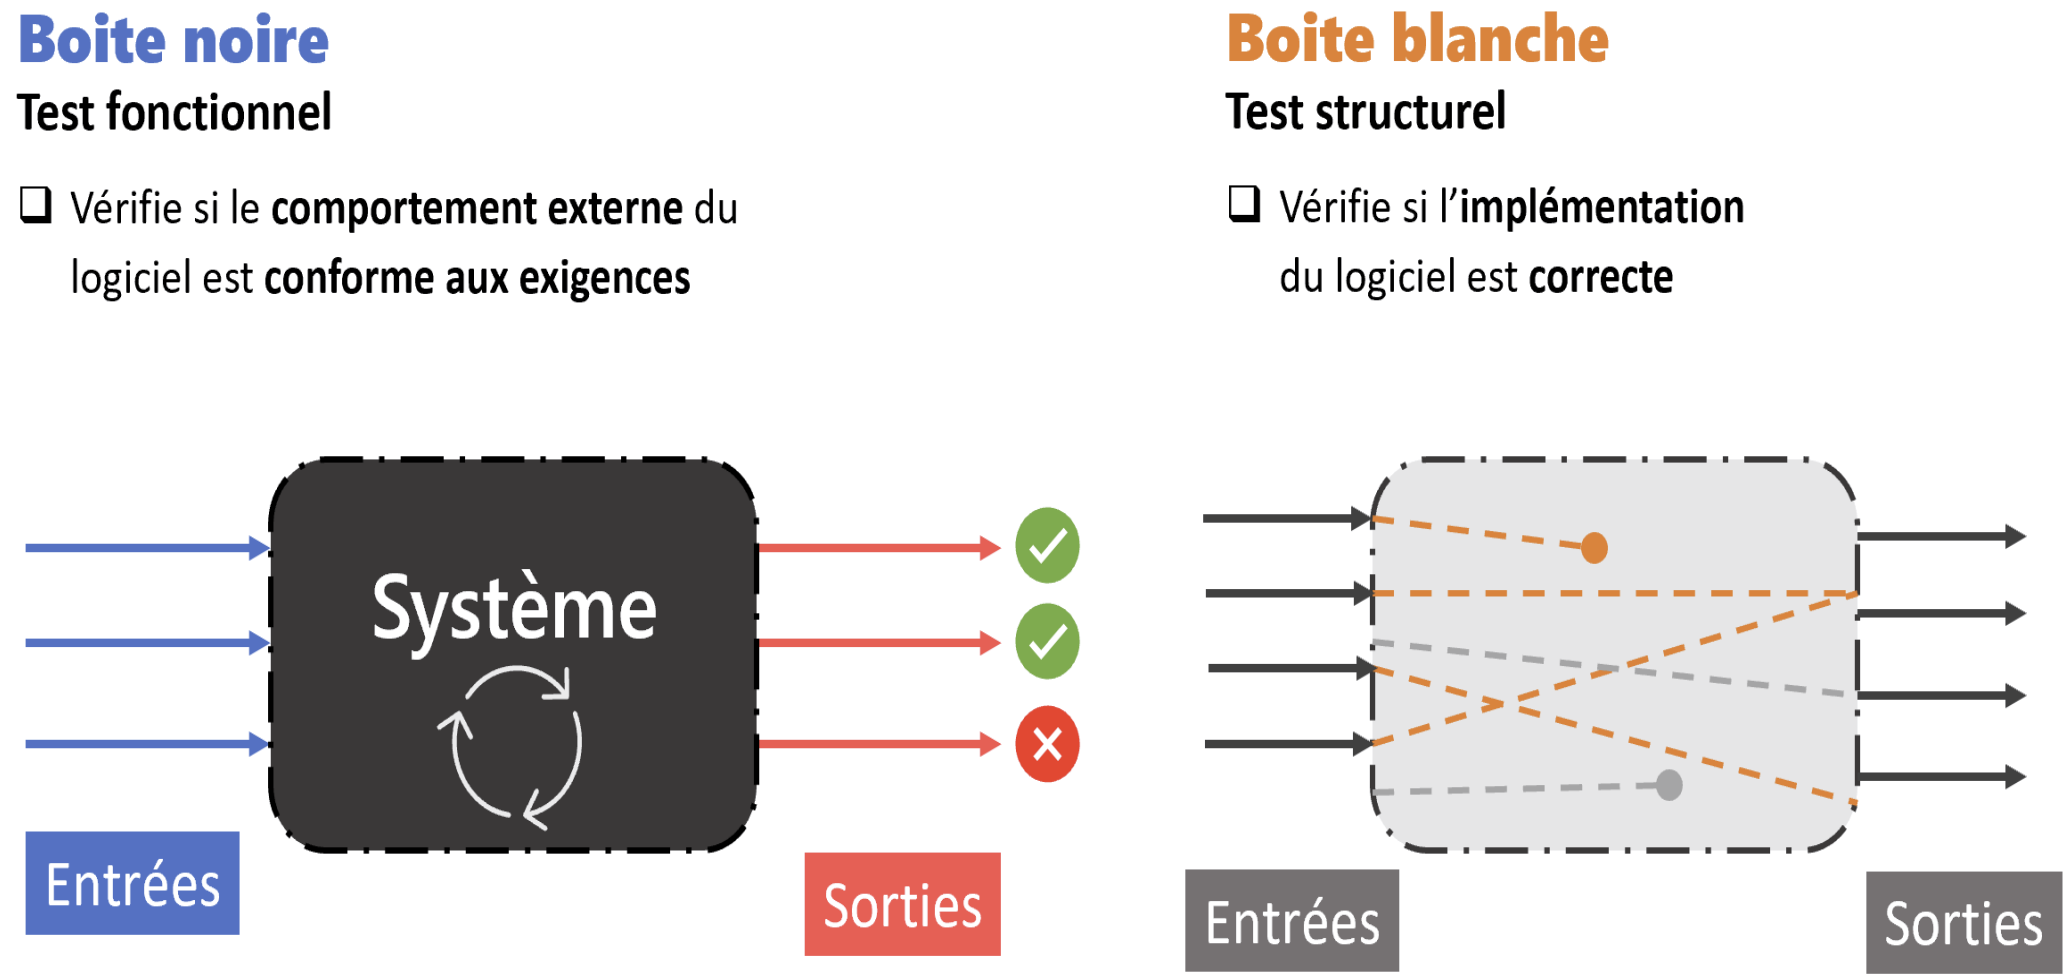
\includegraphics[width=0.45\textwidth]{strattest2.png}
        \end{center}
       \end{figure}
 


        \begin{figure}[H]
        \begin{center}
            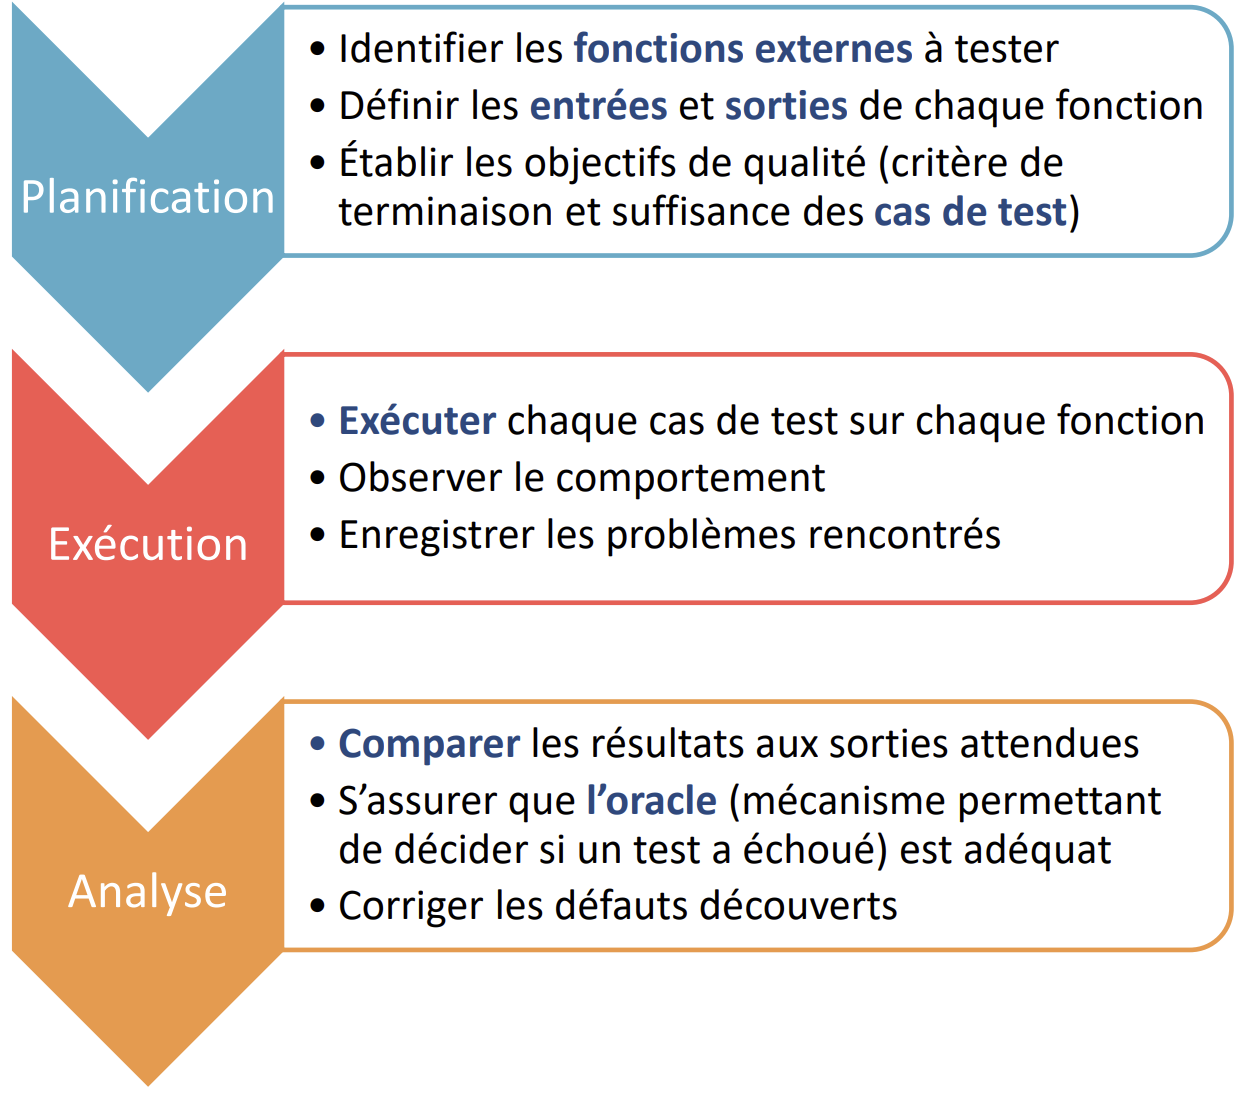
\includegraphics[width=0.45\textwidth]{strattest3.png}
        \end{center}
       \end{figure}


       \section{Comment sélectionner les cas de test}

       Il faut considérer un \textbf{petit ensemble} de cas de tests générables qui sont \textbf{significatifs}. 
       L'objectif est de \textit{maximiser les chances de détecter une faute} et de 
       \textit{minimiser les chances de gaspiller les cas de test}. 
       \begin{note}{}{}
           Chaque test doit \textbf{détecter une faute uneique} qui ne serait pas détectée par un autre. 
       \end{note}               


       \section{Boîte blanche : tester tous les chemins possibles du code} 



       \begin{figure}[H]
        \begin{center}
            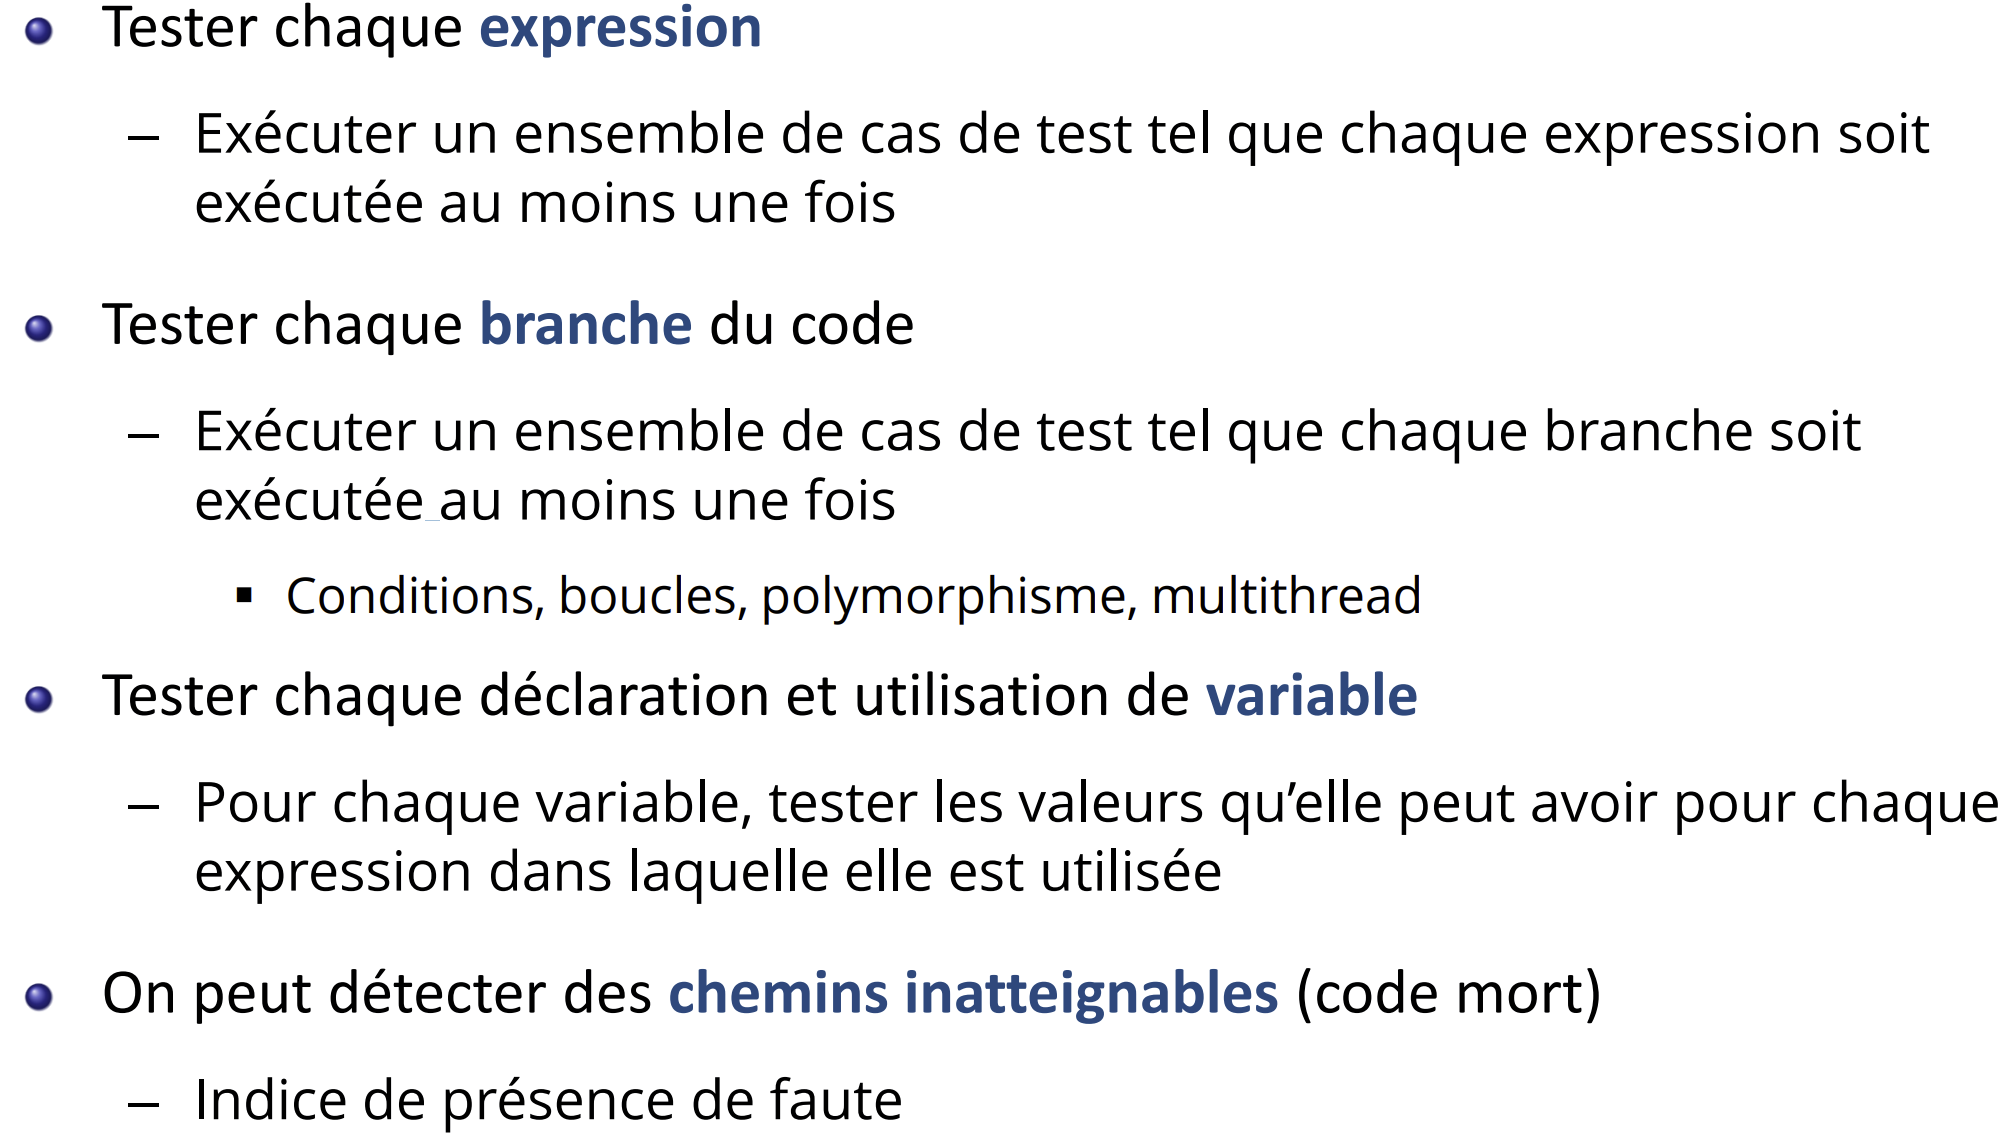
\includegraphics[width=0.45\textwidth]{Stratblanche}
        \end{center}
       \end{figure}

       \begin{Concept}{Test en présence de dépendance}{}
           La plupart des modules requière d'autres modules pour leur bon fonctionnement. 
           Idéalement, chaque module \textbf{doit être testé en isolation} ; cela 
           \textit{facilite le débogage} en permettant une meilleure organisation des tests. 
           Pour isoler une module, on crée des \textbf{modules synthétiques} pour lequels il est dépendants. 
           Par exemple, un faux module pourrait retourner une valeur prédéterminée dont le module à tester 
           va se servir. 
       \end{Concept}


       \section{Types de tests}


       \begin{figure}[H]
        \begin{center}
            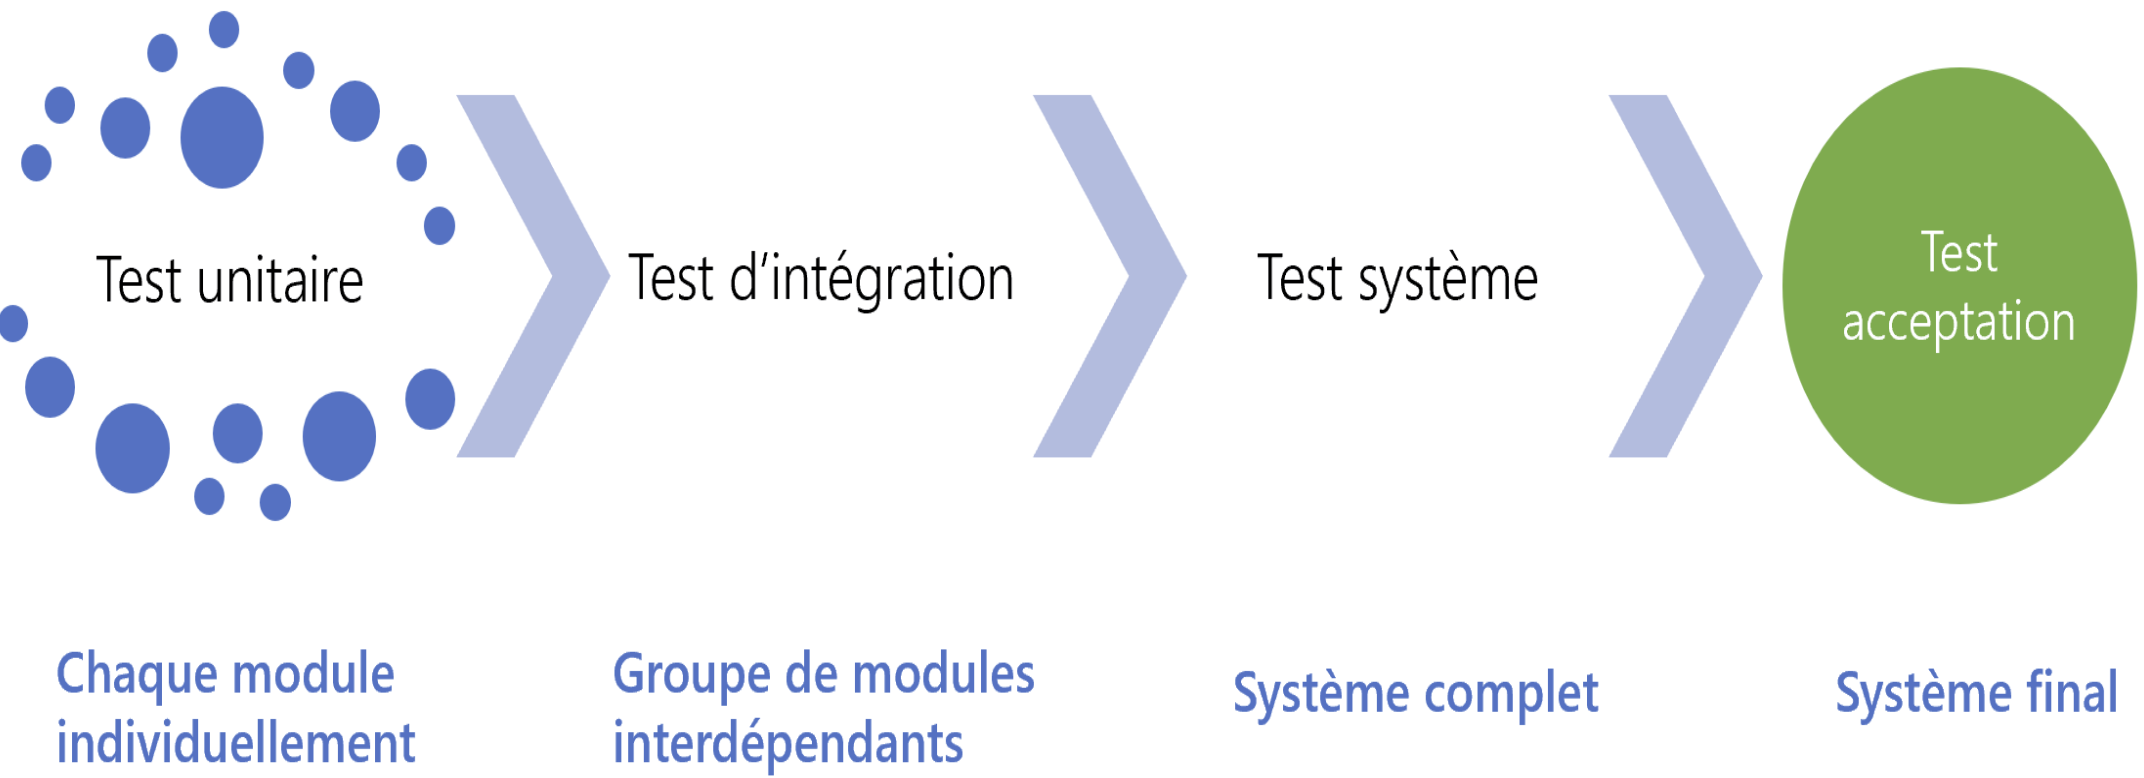
\includegraphics[width=0.45\textwidth]{TypeDeTest.png}
        \end{center}
       \end{figure}


       \begin{itemize}
        \item \textbf{Tests unitaires}  
            \begin{itemize}
                \item[$\blacktriangleright$] Ils vérifient chaque module individuellement 
            \end{itemize}
       \end{itemize}

            

       \begin{figure}[H]
        \begin{center}
            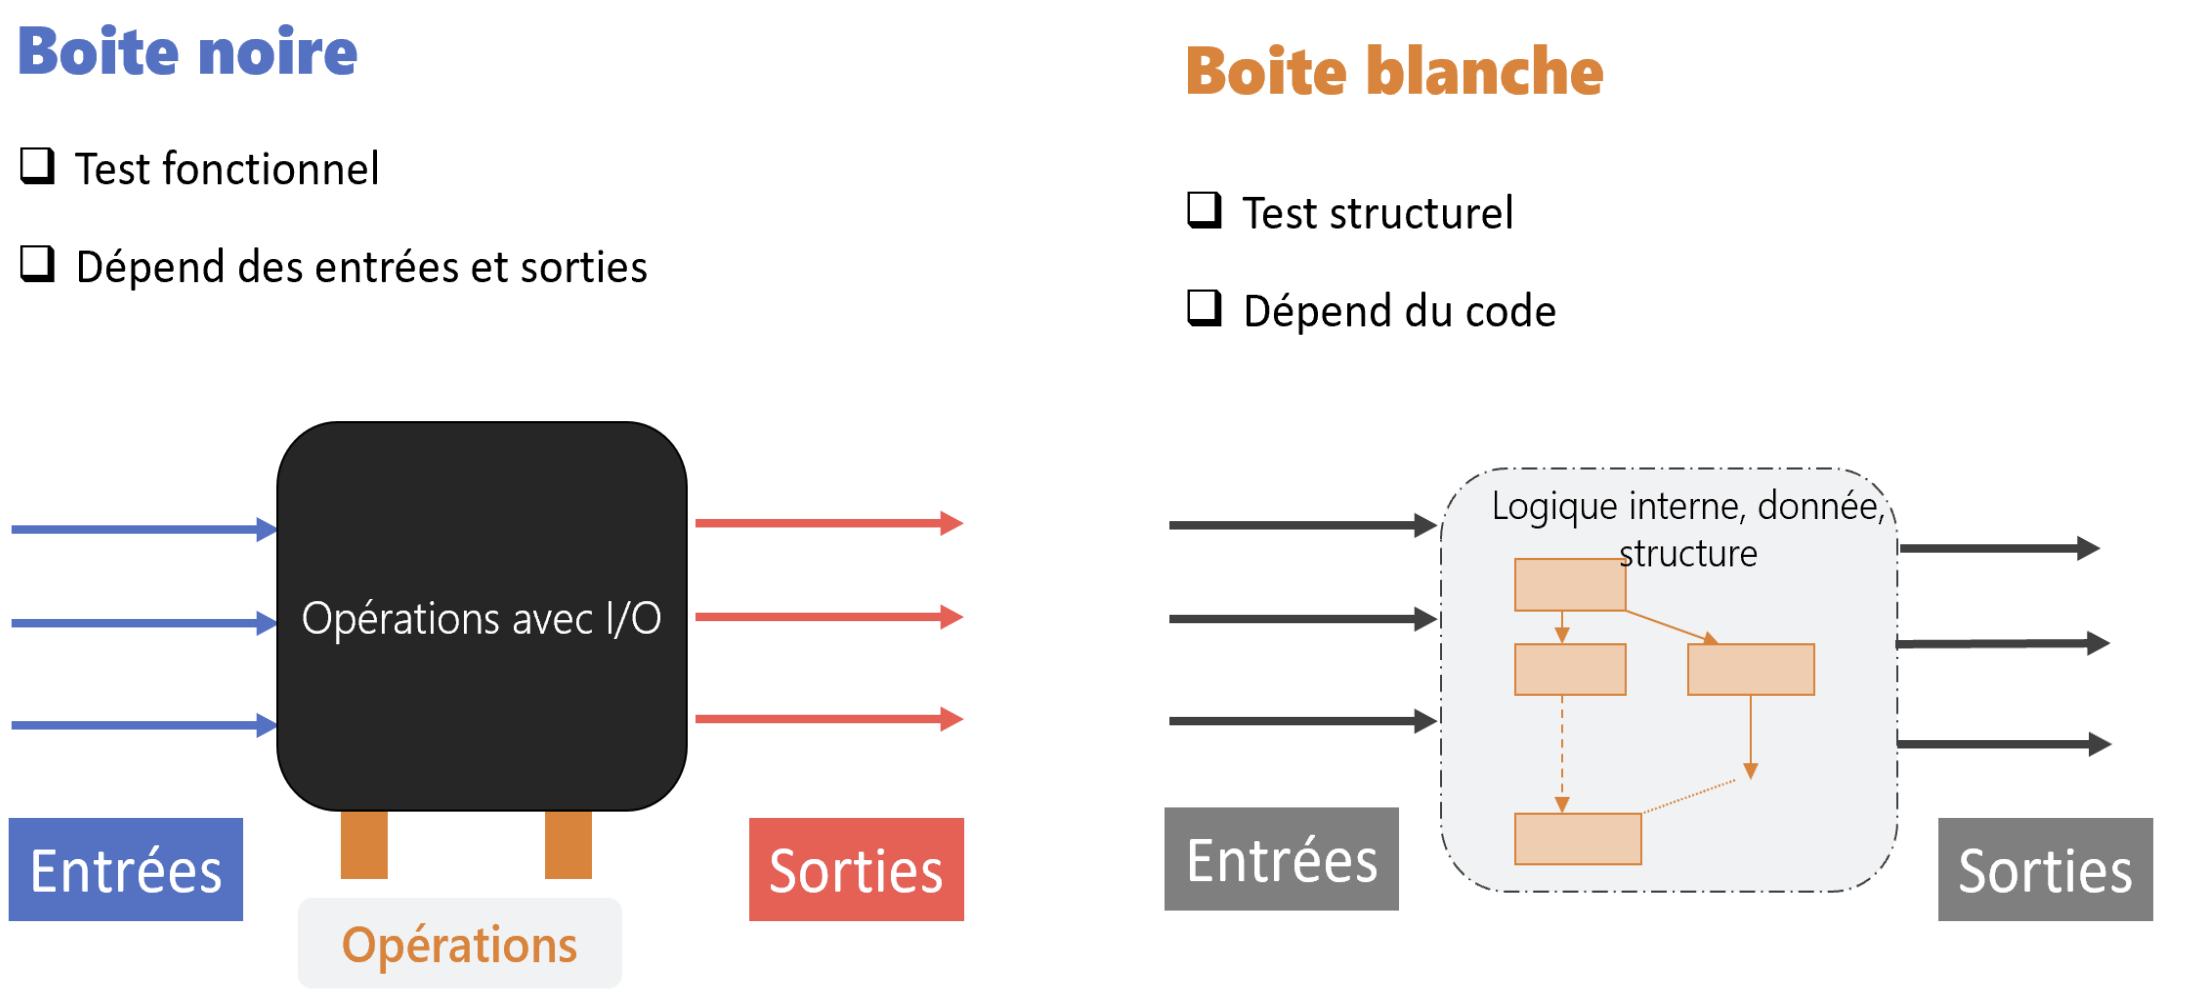
\includegraphics[width=0.45\textwidth]{test1.png}
        \end{center}
       \end{figure}
       

       \begin{itemize}
        \item \textbf{Tests d'intégration}  
            \begin{itemize}
                \item[$\blacktriangleright$] Ils vérifient les intéractions entre plusieurs modules
                \item[$\blacktriangleright$] Utilisé lors de l'ajout de nouveaux modules au groupe de 
                    modules existants
                \item[$\blacktriangleright$] Attention particulière lors des tests de \texttt{GUI}                  
            \end{itemize}
       \end{itemize}



       \begin{figure}[H]
        \begin{center}
            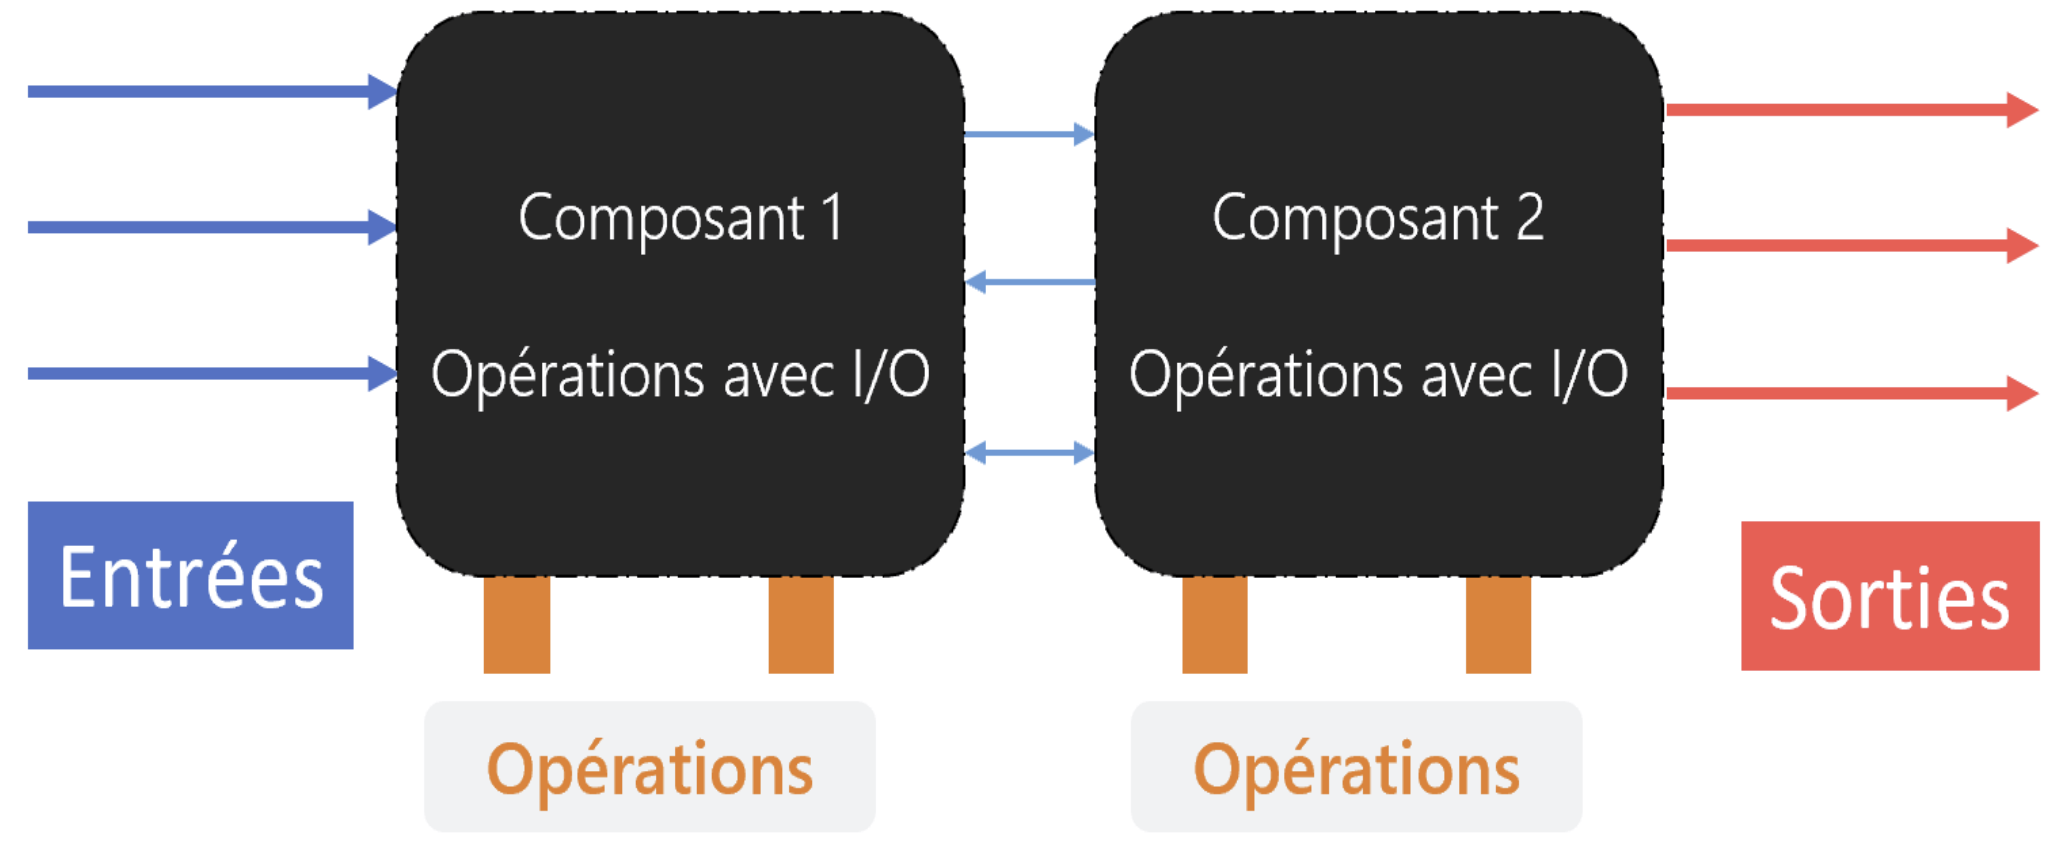
\includegraphics[width=0.45\textwidth]{test2.png}
        \end{center}
       \end{figure}

       \begin{itemize}
        \item \textbf{Tests fonctionnels}  
       \end{itemize}



       \begin{figure}[H]
        \begin{center}
            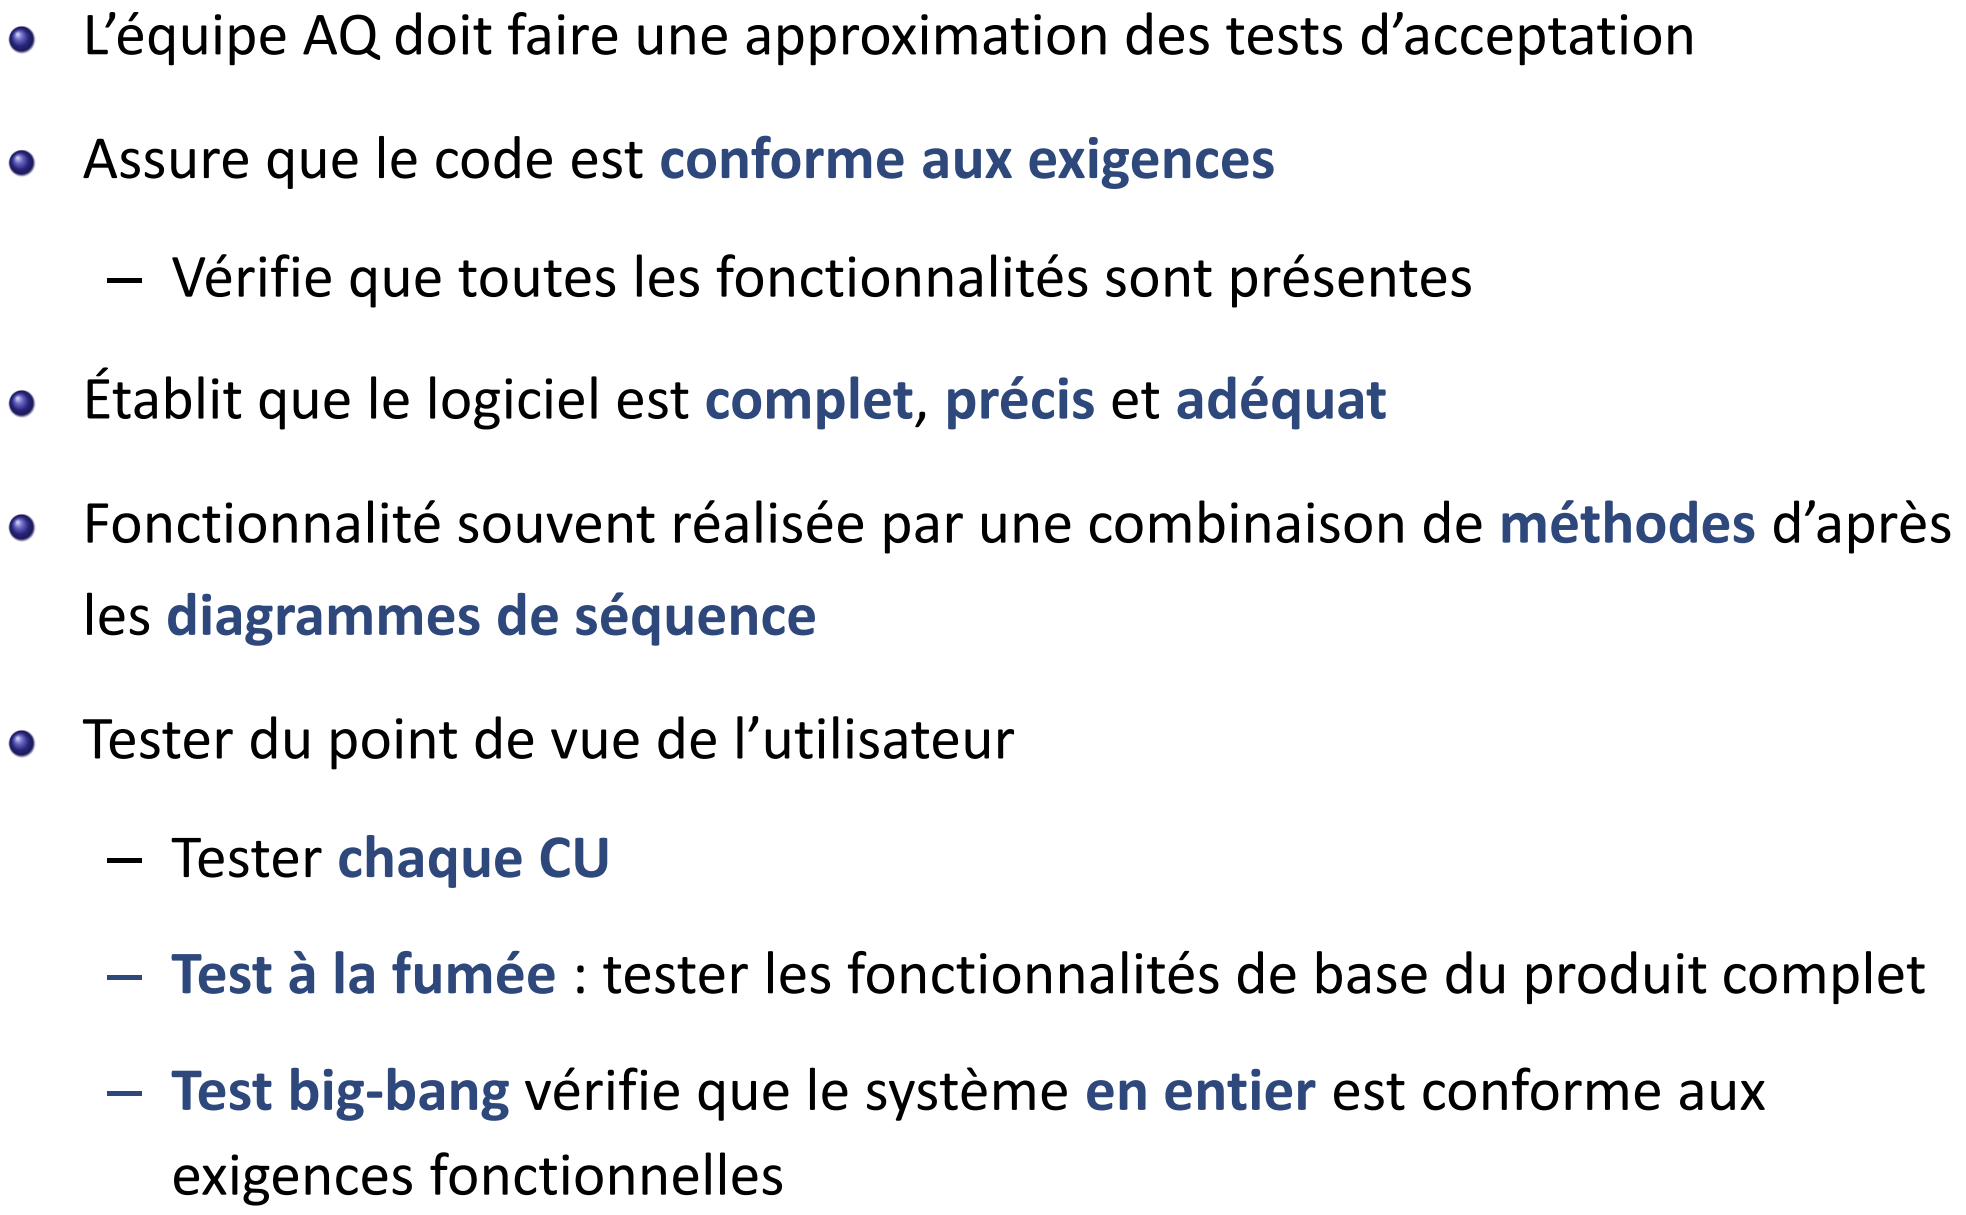
\includegraphics[width=0.45\textwidth]{testfonc1.png}
        \end{center}
       \end{figure}
       
        \begin{itemize}
            \item \textbf{Tests non-fonctionnels}  
        \end{itemize}

       \begin{figure}[H]
        \begin{center}
            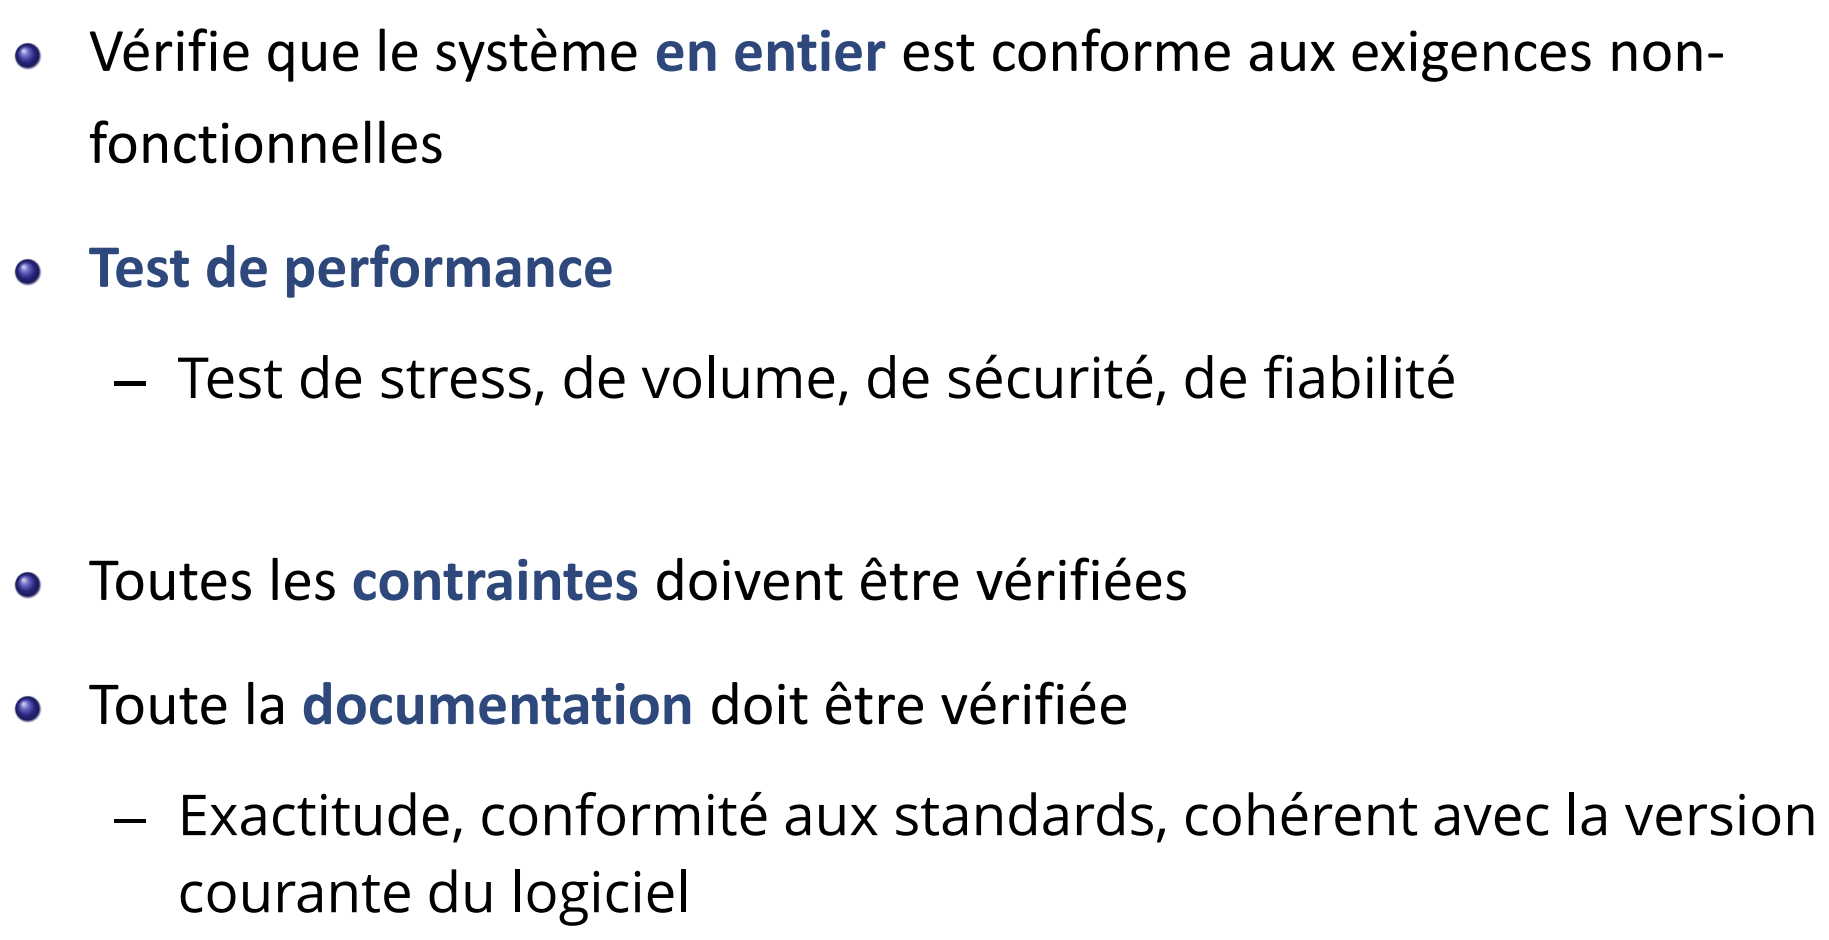
\includegraphics[width=0.45\textwidth]{testfonc2.png}
        \end{center}
       \end{figure}


       




 



    



       
       


       
       



        
        

    






\end{multicols*}








\end{document}
